\documentclass[a4paper]{article}
\usepackage{vntex}
\usepackage{a4wide,amssymb,epsfig,latexsym,multicol,array,hhline,fancyhdr}
\usepackage[table]{xcolor}
\usepackage{pbox}
\usepackage{amsmath}
\usepackage{lastpage}
\usepackage[lined,boxed,commentsnumbered]{algorithm2e}
\usepackage{enumerate}
\usepackage{color}
\usepackage{graphicx}							
\usepackage{array, makecell}
\usepackage{longtable}
\usepackage{tabularx, caption}
\usepackage{multirow}
\usepackage{multicol}
\usepackage{rotating}
\usepackage{graphics}
\usepackage{geometry}
\usepackage{setspace}
\usepackage{epsfig}
\usepackage{tikz}
\usepackage{caption}
\usepackage{subcaption}
\usetikzlibrary{arrows,snakes,backgrounds}
\usepackage{hyperref}
\usepackage{titlesec}
\usepackage{float}
\usepackage{wrapfig}
\usepackage{listings}
\usepackage{rotating}
\graphicspath{{images/}}

\definecolor{dkgreen}{rgb}{0,0.6,0}
\definecolor{gray}{rgb}{0.5,0.5,0.5}
\definecolor{mauve}{rgb}{0.58,0,0.82}
 
\lstset{frame=tb,
  language=HTML,
  aboveskip=3mm,
  belowskip=3mm,
  showstringspaces=false,
  columns=flexible,
  basicstyle={\small\ttfamily},
  numbers=none,
  numberstyle=\tiny\color{gray},
  keywordstyle=\color{blue},
  commentstyle=\color{dkgreen},
  stringstyle=\color{mauve},
  breaklines=false,
  breakatwhitespace=true,
  tabsize=3
}

\restylefloat{figure}
\setcounter{secnumdepth}{4}
\fontsize{10pt}{12pt}
\titleformat{\paragraph}
{\normalfont\normalsize\bfseries}{\theparagraph}{1em}{}
\titlespacing*{\paragraph}
{0pt}{3.25ex plus 1ex minus .2ex}{1.5ex plus .2ex}

\hypersetup{urlcolor=blue,linkcolor=black,citecolor=black,colorlinks=true} 

\newtheorem{theorem}{{\bf Định lý}}
\newtheorem{property}{{\bf Tính chất}}
\newtheorem{proposition}{{\bf Mệnh đề}}
\newtheorem{corollary}[proposition]{{\bf Hệ quả}}
\newtheorem{lemma}[proposition]{{\bf Bổ đề}}

%%%%%%%%%%%JSON Display%%%%%%%%%%%%%%
\colorlet{punct}{red!60!black}
\definecolor{background}{HTML}{ffffff}
\definecolor{delim}{RGB}{20,105,176}
\colorlet{numb}{magenta!60!black}

\definecolor{editorGray}{rgb}{0.95, 0.95, 0.95}
\definecolor{editorOcher}{rgb}{1, 0.5, 0} % #FF7F00 -> rgb(239, 169, 0)
\definecolor{editorGreen}{rgb}{0, 0.5, 0} % #007C00 -> rgb(0, 124, 0)
\usepackage{upquote}
\usepackage{listings}
\lstdefinelanguage{JavaScript}{
  morekeywords={typeof, new, true, false, catch, function, return, null, catch, switch, var, if, in, while, do, else, case, break},
  morecomment=[s]{/*}{*/},
  morecomment=[l]//,
  morestring=[b]",
  morestring=[b]'
}


\lstdefinelanguage{HTML5}{
        language=html,
        sensitive=true, 
        alsoletter={<>=-},
        otherkeywords={
        % HTML tags
        <html>, <head>, <title>, </title>, <meta, />, </head>, <body>,
        <canvas, \/canvas>, <script>, </script>, </body>, </html>, <!, html>, <style>, </style>, ><
        },  
        ndkeywords={
        % General
        =,
        % HTML attributes
        charset=, id=, width=, height=,
        % CSS properties
        border:, transform:, -moz-transform:, transition-duration:, transition-property:, transition-timing-function:
        },  
        morecomment=[s]{<!--}{-->},
        tag=[s]
}

\lstset{%
    % Basic design
    backgroundcolor=\color{background},
    basicstyle={\small\ttfamily},   
    frame=l,
    % Line numbers
    xleftmargin={0.75cm},
    stepnumber=1,
    firstnumber=1,
    numberfirstline=false,
    % Code design   
    keywordstyle=\color{blue}\bfseries,
    commentstyle=\color{darkgray}\ttfamily,
    ndkeywordstyle=\color{editorGreen}\bfseries,
    stringstyle=\color{editorOcher},
    % Code
    language=HTML5,
    alsolanguage=JavaScript,
    alsodigit={.:;},
    tabsize=2,
    showtabs=false,
    showspaces=false,
    showstringspaces=false,
    extendedchars=true,
    breaklines=true,        
    % Support for German umlauts
    literate=%
    {Ö}{{\"O}}1
    {Ä}{{\"A}}1
    {Ü}{{\"U}}1
    {ß}{{\ss}}1
    {ü}{{\"u}}1
    {ä}{{\"a}}1
    {ö}{{\"o}}1
}

\lstdefinelanguage{json}{
    basicstyle=\normalfont\ttfamily,
%    numbers=left,
    numberstyle=\scriptsize,
    stepnumber=1,
    numbersep=8pt,
    showstringspaces=false,
    breaklines=true,
    frame=lines,
    backgroundcolor=\color{background},
    literate=
     *{0}{{{\color{numb}0}}}{1}
      {1}{{{\color{numb}1}}}{1}
      {2}{{{\color{numb}2}}}{1}
      {3}{{{\color{numb}3}}}{1}
      {4}{{{\color{numb}4}}}{1}
      {5}{{{\color{numb}5}}}{1}
      {6}{{{\color{numb}6}}}{1}
      {7}{{{\color{numb}7}}}{1}
      {8}{{{\color{numb}8}}}{1}
      {9}{{{\color{numb}9}}}{1}
      {:}{{{\color{punct}{:}}}}{1}
      {,}{{{\color{punct}{,}}}}{1}
      {\{}{{{\color{delim}{\{}}}}{1}
      {\}}{{{\color{delim}{\}}}}}{1}
      {[}{{{\color{delim}{[}}}}{1}
      {]}{{{\color{delim}{]}}}}{1},
}

\newsavebox\CBox
\def\textBF#1{\sbox\CBox{#1}\resizebox{\wd\CBox}{\ht\CBox}{\textbf{#1}}}

%\usepackage{fancyhdr}
\setlength{\headheight}{40pt}
\pagestyle{fancy}
\fancyhead{} % clear all header fields
\fancyhead[L]{
 \begin{tabular}{rl}
    \begin{picture}(25,15)(0,0)
    \put(0,-8){
\includegraphics[width=8mm, height=8mm]{hcmut.png}}
    %\put(0,-8){\epsfig{width=10mm,figure=hcmut.eps}}
   \end{picture}&
	%
\includegraphics[width=8mm, height=8mm]{hcmut.png} & %
	\begin{tabular}{l}
		\textbf{\bf \ttfamily Trường Đại Học Bách Khoa Tp.Hồ Chí Minh}\\
		\textbf{\bf \ttfamily Khoa Khoa Học và Kỹ Thuật Máy Tính}
	\end{tabular} 	
 \end{tabular}
}
\fancyhead[R]{
	\begin{tabular}{l}
		\tiny \bf \\
		\tiny \bf 
	\end{tabular}  }
\fancyfoot{} % clear all footer field

%FOOTER
\fancyfoot[L]{\scriptsize \ttfamily Luận văn tốt nghiệp - Niên khóa 2016 - 2017}
\fancyfoot[R]{\scriptsize \ttfamily Trang {\thepage}/\pageref{LastPage}}
\renewcommand{\headrulewidth}{0.3pt}
\renewcommand{\footrulewidth}{0.3pt}


%%%
\setcounter{secnumdepth}{4}
\setcounter{tocdepth}{3}
\makeatletter
\newcounter {subsubsubsection}[subsubsection]
\renewcommand\thesubsubsubsection{\thesubsubsection .\@alph\c@subsubsubsection}
\newcommand\subsubsubsection{\@startsection{subsubsubsection}{4}{\z@}%
                                     {-3.25ex\@plus -1ex \@minus -.2ex}%
                                     {1.5ex \@plus .2ex}%
                                     {\normalfont\normalsize\bfseries}}
\newcommand*\l@subsubsubsection{\@dottedtocline{3}{10.0em}{4.1em}}
\newcommand*{\subsubsubsectionmark}[1]{}
\makeatother


\begin{document}

\begin{titlepage}
\begin{center}
ĐẠI HỌC QUỐC GIA THÀNH PHỐ HỒ CHÍ MINH \\
TRƯỜNG ĐẠI HỌC BÁCH KHOA \\
KHOA KHOA HỌC VÀ KỸ THUẬT MÁY TÍNH 
\end{center}

\vspace{1cm}

\begin{figure}[h!]
\begin{center}

\includegraphics[width=3cm]{hcmut.png}
\end{center}
\end{figure}

\vspace{1cm}


\begin{center}
\begin{tabular}{c}
\multicolumn{1}{l}{\textbf{{\Large LUẬN VĂN TỐT NGHIỆP}}}\\
~~\\
\hline
\\
\multicolumn{1}{l}{\textbf{{\Large Đề tài 126}}}\\
\\
\textBF{\Huge Phát triển ứng dụng quản lý}\\
\textBF{\Huge lịch trình đi lại của nhân viên}\\
\\
\hline
\end{tabular}
\end{center}

\vspace{2cm}

\begin{table}[h]
\begin{tabular}{rrll}
\hspace{5 cm} & GVHD: & TS. Phan Trọng Nhân\\
&GVPB:& ThS. Đặng Trần Trí&
\\
& Thành viên: & Nguyễn Đức Vũ Anh & 51300098\\
& & Nguyễn Viết Minh Dũng & 51300678\\
& & Trương Hải Ngọc Đàm & 51300737\\
\end{tabular}
\end{table}

\begin{center}
{\footnotesize TP. HỒ CHÍ MINH, THÁNG 11/2017}
\end{center}
\end{titlepage}

\section*{Lời cảm ơn}
Trong suốt quá trình hoàn thành đề tài luận văn tốt nghiệp này, chúng tôi xin gửi lời cảm ơn chân thành nhất đến thầy   Phan Trọng Nhân, giảng viên hướng dẫn trực tiếp đề tài. Thầy đã tận tình hướng dẫn, theo dõi, cũng như góp ý những sai sót, đánh  giá những mặt làm được đồng thời định hướng trong đề tài chúng tôi thực hiên.\\
\\
Chúng tôi cũng xin gửi lời cảm ơn tới tất cả các thầy cô trong khoa Khoa học và Kỹ thuật Máy tính, đã hết lòng truyền đạt những tri thức, những kiến thức học thuật cũng như kinh nghiệm quý báu cho chúng tôi trong suốt quá trình học tập tại trường.\\
\\
Trong suốt quá trình luận văn tốt nghiệp, chúng tôi khó tránh khỏi sai sót, rất mong thầy cô thông cảm. Đồng thời vì kinh nghiệm thực tiễn còn hạn chế nên bài báo cáo thực tập không tránh những thiếu sót, chúng tôi rất mong được sự góp ý của thầy cô, để trau dồi học hỏi nhiều hơn, đồng thời hoàn thành tốt hơn trong giai đoạn Luận văn tốt nghiệp sắp tới.\\
\\
Chúng tôi xin chân thành cảm ơn!\\
\\
\begin{flushright}
    TP. Hồ Chí Minh, tháng 11 năm 2017 \\
                  
\end{flushright}
\begin{flushright}
    \textbf{Nhóm sinh viên thực hiện đề tài}
\end{flushright}

%MỤC LỤC
\newpage
\tableofcontents
\newpage
%DANH MỤC HÌNH ẢNH
\listoffigures
\newpage
%DANH MỤC BẢNG
\listoftables
\newpage
\section*{Danh sách thuật ngữ và khái niệm}
\begin{table}[h]
    \centering
    \begin{tabular}{|c|l|m{6cm}|}
        \hline
        \thead{\textbf{Thuật ngữ}} & \thead{\textbf{Tên đầy đủ}} & \thead{\textbf{Ghi chú}} \\
        \hline
        API&Application Programming Interface&Giao diện mà một hệ thống máy tính hay ứng dụng cung cấp để cho phép các yêu cầu dịch vụ có thể được tạo ra từ các chương trình máy tính khác, hoặc cho phép dữ liệu có thể được trao đổi qua lại giữa chúng.\\
        \hline
        HTTP & HyperText Transfer Protocol & Giao thức truyền tải siêu văn bản – là một trong năm giao thức chuẩn về mạng Internet, được dùng để liên hệ thông tin giữa máy cung cấp dịch vụ và máy sử dụng dịch vụ.\\
        \hline
        VPS & Virtual Private Server & Là dạng máy chủ ảo được tạo ra bằng phương pháp phân chia một máy chủ vật lý thành nhiều máy chủ khác nhau có tính năng tương tự như máy chủ riêng, chạy dưới dạng chia sẻ tài nguyên từ máy chủ vật lý ban đầu.\\
        \hline
        URL  & Uniform Resource Locator & Định vị tài nguyên thống nhất – được dùng để tham chiếu tới tài nguyên trên Internet.\\
        \hline
        GPS & Global Positioning System & Hệ thống định vị toàn cầu.\\
        \hline
        MVC & Model-View-Controller & Mẫu kiến trúc phần mềm, chia ứng dụng thành 3 phần đóng vai trò riêng biệt.\\
        \hline
        JSON & JavaScript Object Notation & Một kiểu dữ liệu mở nguồn gốc từ Javascript.\\
        \hline
        XML & eXtensible Markup Language &  Ngôn ngữ đánh dấu mở rộng.\\
        \hline
        REST & Representational state transfer & Một mô hình cung cấp khả năng tương tác giữa các hệ thống máy tính trên thế giới.\\
        \hline
    \end{tabular}
\end{table}  
\newpage
%%%%%%%%%%%%%%%%%%%%
%%%%%%%%%%%%%%%%%%%%
\section{Giới thiệu} 
\subsection{Giới thiệu đề tài}
Hiện nay, trong quá trình hội nhập và toàn cầu hóa, các doanh nghiệp luôn luôn đẩy mạnh các đàm phán, giao dịch, trao đổi với khách hàng. Vấn đề đi lại, di chuyển công tác của nhân viên là một việc thiết yếu, để giảm thiểu, tối ưu hóa chi phí cho doanh nghiệp, việc quản
lí lịch trình đi lại của nhân viên là điều cần thiết.\\
\\
Hầu hết chi phí đi lại liên quan tới công việc của nhân viên đều được quyết toán tại bộ phận quản lý tài chính của doanh nghiệp. Các thủ tục phân công và minh chứng nhân viên đi công tác đều thông qua giấy tờ, hoặc trực tiếp. Hạn chế trong những thủ tục này là phức tạp,
phải cần thời gian chờ sự chấp thuận của các phòng ban, việc minh chứng để thanh toán chi phí đi lại trong quá trình công tác chưa nhanh gọn, cần nhiều công sức của bộ phận quản lí tài chính của doanh nghiệp.\\
\\
Để giúp đỡ, tăng hiệu suất công tác quản lý, tăng tính tự động hóa, chúng tôi hướng đến việc xây dụng một ứng dụng mobile quản lý lịch trình đi lại của nhân viên. Ứng dụng tập trung vào việc: các trưởng phòng ban có thể sắp xếp, phân công lịch trình đi lại công tác của
nhân viên, nhân viên nhận và thực hiên lịch trình, hệ thống theo dõi lịch trình đi lại của nhân viên theo GPS và dự đoán chi phí đi lại, nhân viên có thể minh chứng cho chi phí đi lại của mình.
\subsection{Mục tiêu đề tài}
\subsubsection{Giai đoạn thực tập tốt nghiệp}
\begin{itemize}    
    \item Tìm hiểu nghiệp vụ của lịch trình đi lại của nhân viên
    \item Phân tích chi tiết và giải pháp các vấn đề trong ứng dụng quản lí lịch trình đi lại
    \item Thiết kế các tính năng của ứng dụng
    \item Thiết kế usecase, sequence diagram, cơ sở dữ liệu, kiến trúc hệ thống, thiết kế giao diện cho ứng dụng
    \item Tìm hiểu công nghệ Google Maps API; công nghệ Java, Spring Framework để xây dựng hệ thống server; công nghệ Java Android để xây dựng ứng dụng trên mobile
\end{itemize}
\subsubsection{Giai đoạn luận văn tốt nghiệp}
\begin{itemize}    
    \item Thiết kế activity diagram
    \item Xây dựng bộ kiểm thử hệ thống (testcase)
    \item Hiện thực server để quản lý ứng dụng
    \item Hiện thực các tính năng của ứng dụng trên mobile
    \item Xây dựng ứng dụng dễ sử dụng, thân thiện với người dùng
\end{itemize}
\subsection{Phạm vi của đề tài}
Ứng dụng được áp dụng cho nhân viên trong công ty. Ứng dụng hoạt động trên nền tảng mobile chạy hệ điều hành Android, cần sử dụng GPS.
\subsection{Cấu trúc báo cáo}
Nội dung của báo cáo luận văn tốt nghiệp được trình bày gồm:
\begin{itemize}    
    \item Chương 1: Giới thiệu đề tài
    \item Chương 2: Cơ sở lí thuyết và nền tảng công nghệ
    \item Chương 3: Phân tích yêu cầu và chức năng ứng dụng
    \item Chương 4: Thiết kế dựa trên tài liệu đã phân tích ở chương 3
    \item Chương 5: Hiện thực 
    \item Chương 6: Tổng kết
    \item Danh mục tài liệu tham khảo
    \item Danh mục hình ảnh
    \item Danh mục bảng 
\end{itemize}

%%%%%%%%%%%%%%%%%%%%%%%%%%%%%%%%%%%%%%%%%%%%%%%
%%%%%%%%%%%%%%%%%%%%%%%%%%%%%%%%%%%%%%%%%%%%%%%
\section{Cơ sở lý thuyết và nền tảng công nghệ}
\textit{Trong chương này, chúng tôi sẽ giới thiệu chi tiết về công nghệ GoogleMap API, công nghệ nền tảng trong hệ thống của chúng tôi. Bên cạnh đó chúng tôi cũng sẽ giới thiệu về công nghệ mà chúng tôi sử dụng để hiện thực hệ thống back-end là ngôn ngữ NodeJS và Framework Express.}
\subsection{Công nghệ Google Map API}
\subsubsection{Google Map API là gì?}
Google Map là một dịch vụ ứng dụng vào công nghệ bản đồ trực tuyến trên web miễn phí được cung cấp bởi Google, giúp cho ta có thể dò đường, xem bản đồ, tìm các tuyến đường tối ưu, cách bắt xe buýt... trên toàn thế giới.\\
\\
Map API là một phương pháp giúp cho website ta đang xây dựng có khả năng tích hợp dịch vụ bản đồ của một trang web khác (ở đây là Google).\\
\\
Các ứng dụng xây dựng trên maps được nhúng vào trang web cá nhân thông qua các thẻ Javascripts do vậy việc sử dụng API Google rất dễ dàng.\\
\\
Một số ứng dụng của Google Map API:
\begin{itemize}    
    \item Đánh dấu các địa điểm trên bản đồ kèm theo thông tin cho địa điểm đó: khu vui chơi giải trí, nhà hàng khách sạn, cây ATM, bệnh viện, trường học, ...
    \item Chỉ dẫn đường đến các địa điểm cần tìm (đường tối ưu và nhiều option khác), chỉ dẫn đường giao thông công cộng, có thể là các địa điểm cung cấp như trên. Ở đây sử dụng các service google cung cấp.
    \item Khoanh vùng khu vực: các trung tâm kinh tế, khu đô thị, khu ô nhiễm ... 
    \item Tình trạng giao thông các khu vực, từ đó đưa ra các giải pháp ...    
\end{itemize}

\subsubsection{Tạo một Google Map đơn giản}
\begin{itemize}    
    \item[-] Tạo 1 API Key
    \begin{itemize}
        \item[•] Truy cập vào \url{https://code.google.com/apis/console} và đăng nhập bằng tài khoản gmail của mình.
        \item[•] Click \texttt{the APIs \& auth $\rightarrow$ APIs}.
        \item[•] Kéo xuống dưới tìm \texttt{Google Maps JavaScript API v3} và kích hoạt dịch vụ bằng việc click vào button chuyển trạng thái từ \textbf{OFF} sang \textbf{ON}.
        \item[•] Click \texttt{API Access $\rightarrow$ Create new Browser key...}, một API key sẽ hiện lên và bạn sẽ copy lại để sử dụng.
    \end{itemize}
    \begin{figure}[h]
        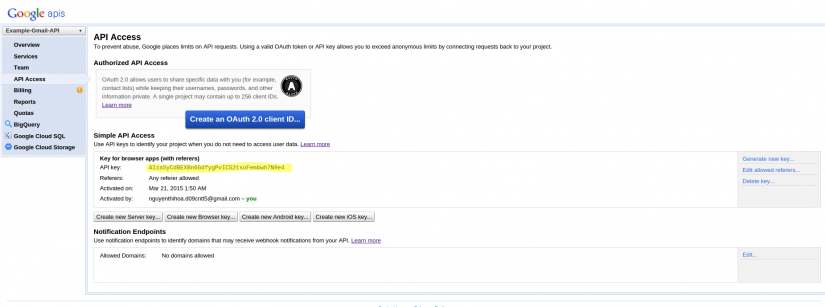
\includegraphics[scale=0.6]{gmap_api}
        \centering
        \caption{Tạo API Key Google maps}
        \label{fig:gmap_api}
    \end{figure}
    \item[-] Lấy kinh độ, vĩ độ để hiển thị bản đồ\\
     Truy cập vào \url{http://www.latlong.net} và nhập địa điểm cần tìm.
    \item[-] Hiển thị bản đồ
%    \begin{figure}[h]
%        \includegraphics[scale=0.6]{gmap_display}
%        \centering
%        \caption{Hiển thị bản đồ google maps}
%        \label{fig:gmap_display}
%    \end{figure}
\begin{lstlisting}
// Doan code hien thi ban do Google Map
<html>
  <head>
    <script src="http://maps.googleapis.com/maps/api/js?key=#{your_app_key}
    &censor=false"></script>
    <script>
      // Khoi tao Map
      function initialize() {
        // Khai bao cac thuoc tinh
        var mapProp = {
          // Tam ban do, quy dinh boi kinh do va vi do
          center:new google.maps.LatLng(51.508742, -0.120850),
          // Set default zoom cua ban do khi duoc load
          zoom:5,
          // Dinh nghia type
          mapTypeId:google.maps.MapTypeId.ROADMAP
        };
        // Truyen tham so cho cac thuoc tinh Map cho the div chua Map
        var map = new google.maps.Map(document.getElementById("googleMap"), mapProp);
      }
      google.maps.event.addDomListener(window, 'load', initialize);
    </script>
  </head>
  <body>
    <!-- Khai bao the div chua Map -->
    <div id="googleMap" stype="width:500px;height:380px;"></div>
  </body>
</html>
\end{lstlisting}
\end{itemize}
\subsection{Công nghệ Java}
\subsubsection{Java là gì}
Java là một ngôn ngữ lập trình được sử dụng rộng rãi được phát triển bởi Sun Microsystems vào năm 1995. Java có tính bảo mật cao và là một ngôn ngữ lập trình hướng đối
tượng. Đồng thời, một chương trình biết bằng Java có thể chạy được trên nhiều nền tảng và thiết bị khác nhau, cho phép người lập trình sử dụng một chương trình cho nhiều
nền tảng.

\subsubsection{Ưu điểm của Java}
Đầu tiên, Java là một ngôn ngữ lập trình hướng đối tượng, nghĩa là Java sử dụng các đối tượng được định nghĩa đầy đủ và mối quan hệ giữa các đối tượng khác nhau để thực
hiện các tác vụ khác nhau. Ngoài ra, Java còn sở hữu mọi ưu điểm của ngôn ngữ hướng đối tượng (có thể dùng lại code và mở rộng,...)\\\\
Thứ hai, Java là một ngôn ngữ đa nền tảng, sử dụng Java bytecode và Java Virtual Machine (JVM). Không như những ngôn ngữ khác được biên dịch trực tiếp thành mã máy trên
một nền tảng cụ thể, code Java sẽ được biên dịch thành một định dạng trung gian (bytecode) và được thực thi bởi JVM. Ta có thể viết một chương trình Java trên máy Windows
và thực thi nó trên máy Linux hoặc Mac OS, chỉ cần hai máy này có cài đặt môi trường Java.
\subsubsection{Nhược điểm của Java}
Nhược điểm lớn nhất của Java là tốc độ của nó chậm hơn so với các ngôn ngữ khác (PHP, ASP.NET..). Ngoài ra, ngôn ngữ Java tương đối khó để học đối với những người mới bắt
đầu học lập trình.
\subsection{Spring Framework }
Spring là một framework được viết bằng Java, Spring cung cấp cho người dùng nền tảng để phát triển ứng dụng Java. Spring cho phép người dùng xây dựng các ứng dụng từ các
“đối tượng Java cổ điển (POJOs)”, sau đây là một số ưu điểm của Spring:
   \begin{itemize}
     \item Là một framework tương đối nhẹ (lighweigth).
     \item Được sử dụng nhiều cho các ứng dụng web vì hỗ trợ rất tốt các tính năng như web serices hay json...
     \item Hỗ trợ quản lý transaction, JDBC operations, File uploading, Exception Handling....
   \end{itemize}
\subsection{Mô hình MVC}
MVC là  viết tắt của Model-View-Controller. MVC là một mẫu kiến trúc phần mềm trong công nghệ phần mềm. Mô hình MVC, khi sử dụng đúng cách, sẽ giúp cho người phát triển phần mềm phân tách giữa logic của quy trình nghiệp vụ với giao diện người dùng một cách rõ ràng hơn.\\
\\
Trong mô hình MVC, gồm ba thành phần:
\begin{itemize}
    \item Model: là thành phần trung tâm của mô hình. Nó diễn tả những hành vi của ứng dụng trong giới hạn những vấn đề ứng dụng giải quyết, không phụ thuộc vào giao diện. Nó trực tiếp quản lí dữ liệu, logic, và những quy tắc của chương trình.
    \item View: bao gồm các thành phần giao diện của ứng dụng, có thể là bất kì đại diện đầu ra của thông tin, chẳng hạn như một biểu đồ, thống kê… cũng như là nơi gửi hành động của người dùng đến Controller.
    \item Controller: là nơi kiểm tra dữ liệu đầu vào, quản lí sự trao đổi giữa dữ liệu và các quy tắc trong chương trình.
\end{itemize}
Sự tương tác giữa các thành phần được thể hiện ở hình \ref{fig:mvc}.
\begin{figure}[h]
  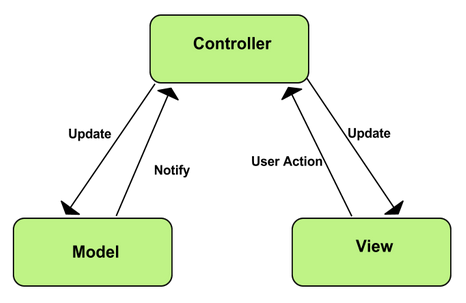
\includegraphics[scale=0.8]{mvc}
  \centering
  \caption{Tương tác trong mô hình MVC}
  \label{fig:mvc}
\end{figure}
\subsection{JSON}
Giới thiệu JSON:\\
\\
JSON là viết tắt của JavaScript Object Notation. Chúng dễ dàng đọc và viết. Chúng là cơ sở dựa trên tập hợp của ngôn ngữ Javascript, tiêu chuẩn  ECMA-262 phiên bản 3 - tháng 12 năm 1999. JSON là một kiểu dữ liệu độc lập, có thể  trao đổi dữ liệu có cấu trúc giữa các ngôn ngữ lập trình mà không phụ thuộc bất cứ ngôn ngữ nào, nó cùng là một kiểu dữ liệu dễ dàng được dùng để gửi và nhận  giữa server và client với nhau.\\
\\
Cấu trúc của JSON dựa trên các cặp Key/Value:
\begin{itemize}
    \item Key là một chuỗi
    \item Value có thể là chuỗi, số, giá trị Boolean, mảng, object …
\end{itemize}
Một JSON Object bao gồm cặp Key/Value và được bắt đầu bởi dấu "\{" và kết thúc bởi dấu "\}".\\
\\
\textbf{Ví dụ:} Sử dụng JSON để mô tả đối tượng 1 Student:
\begin{lstlisting}[language=json,firstnumber=1]
{
	"student_id" :  1,
	"name" : "Nguyen Van A",
	"male": true,
	"class": ["guitar","piano"]
}
\end{lstlisting}
\textbf{Ví dụ 2:} Sử dụng JSON để mô tả danh sách các đối tượng Student:
\begin{lstlisting}[language=json,firstnumber=1]
[
  {
    	"student_id" :  1,
    	"name" : "Nguyen Van A",
    	"male": true,
    	"class": ["guitar","piano"]
   },
   {
      "student_id" :  1,
      "name" : "Nguyen Thi B",
      "male": false,
      "class": ["guitar","piano","cheese"]
   }
]
\end{lstlisting}
\subsection{Android}
Là hệ điều hành mã nguồn mở và dựa trên Linux, dành cho các thiết bị mobile như Smartphone và máy tính bảng. Android đưa ra một phương pháo thống nhất để phát triển ứng dụng cho các thiết bị di động, và các ứng dụng có thể chạy trên nhiều ứng dụng khác nhau đã được cài Android Studio.
%%%%%%%%%%%%%%%%%%%%%%%%%%%%%%%%%%%%%%%%%%%%%%%%%
%%%%%%%%%%%%%%%%%%%%%%%%%%%%%%%%%%%%%%%%%%%%%%%%%
\section{Phân tích yêu cầu và chức năng ứng dụng}
\subsection{Mô tả nghiệp vụ}
\subsubsection{Quy trình nghiệp vụ ban đầu khi chưa có hệ thống}
Ứng dụng này được thiết kế cho các công ty để quản lý lịch trình đi lại của nhân viên, ba đối tượng chính trong ứng dụng là nhân viên, quản lý và người quản trị.\\
\\
Nhân viên sẽ là những người được giao và thực hiện cuộc hẹn. Các nhân viên sẽ được quản lý bởi người quản lý.\\
\\
Người quản lý là những người quản lý các nhân viên của mình, họ có trách nhiệm tạo một cuộc hẹn mới, gán cuộc hẹn mới đó cho các nhân viên mà họ quản lý hoặc tự thực hiện lịch trình.\\
\\
Người quản trị là những người quản lý hệ thống, họ có nhiệm vụ cấp tài khoản cho những người sử dụng (nhân viên và người quản lý), đồng thời họ cũng có thể xem và quản lý dữ liệu (lịch sử đi lại, danh sách người dùng ...) trong hệ thống.\\
\\
Đầu tiên, người quản lý sẽ đăng ký các cuộc hẹn. Khi có cuộc hẹn được gán cho nhân viên, nhân viên sẽ nhận thông báo chi tiết về công việc, ứng dụng sẽ có thông báo đến người dùng khi gần đến thời gian bắt đầu cuộc hẹn.\\
\\
Trước khi bắt đầu cuộc hẹn, nhân viên sẽ phải thông báo phương tiện mà mình chọn để di chuyển cho công ty.
Sau khi đến nơi, nhân viên thông báo kết thúc lịch trình và thông báo chi phí đi lại cho công ty, nếu phương tiện đó có xuất ra hóa đơn thì nhân viên đem hóa đơn đó nộp về công ty.
\subsubsection{Quy trình thực hiện}
\begin{itemize}    
    \item[-] Các bước chính trong việc sử dụng ứng dụng quản lý lịch trình  
    \begin{itemize}  
        \item[•] Đăng nhập vào hệ thống
        \item[•] Xem danh sách các cuộc hẹn với khách hàng
        \item[•] Chọn một cuộc hẹn trong danh sách
        \item[•] Chọn phương tiện di chuyển 
        \item[•] Chọn chức năng bắt đầu khi bắt đầu xuất phát
        \item[•] Chọn chức năng kết thúc khi hoàn thành công việc
        \item[•] Chọn gửi ảnh chụp hóa đơn và giá tiền được nhập về cho hệ thống
    \end{itemize}
    \item[-] Riêng đối với admin thì có quy trình nghiệp vụ như sau 
    \begin{itemize}  
        \item[•] Đăng nhập vào trang quản trị
        \item[•] Thực hiện các chức năng quản lý nhưa: tạo và cấp phát tài khoản, kích hoạt hoặc vô hiệu hóa tài khoản, xem thông tin lịch sử lịch trình đi lại và danh sách các cuộc hẹn hiện tại của người dùng.
    \end{itemize}  
\end{itemize}
\subsubsection{Quy trình chi tiết}
\begin{itemize}    
    \item[-] Đăng nhập vào hệ thống: \par
    Hệ thống yêu cầu nhân viên bắt buộc phải đăng nhập trước khi sử dụng. Mỗi nhân viên của công ty sẽ được admin cấp phát cho một tài khoản đăng nhập. Ở phần đăng nhập, nhân viên nhập username và password đã được admin cấp phát để đăng nhập vào hệ thống. Ngoài ra hệ thống có hỗ trợ chức năng đổi mật khẩu để nhân viên thay đổi mật khẩu theo ý mình.
    \item[-] Xem danh sách các cuộc hẹn với khách hàng: \par
    Sau khi đăng nhập thành công, tại trang home của ứng dụng nhân viên sẽ được xem danh sách cuộc hẹn. Các cuộc hẹn trong danh sách được sắp xếp theo thứ tự thời gian từ sớm nhất đến trễ nhất để nhân viên lựa chọn cuộc hẹn một cách hợp lý. Mỗi cuộc hẹn trong mục này bao gồm những thông tin chính sau: Mã khách hàng, tên khách hàng, nội dung công việc, thời gian hẹn, địa điểm hẹn. Nếu user là manager thì có thêm quyền tạo cuộc hẹn mới và có thể phân phối xuống cho nhân viên cấp dưới của mình thực hiện. Cuộc hẹn được phân phối sẽ tự động được thêm vào danh sách cuộc hẹn của nhân viên.
    \item[-] Chọn một cuộc hẹn trong danh sách:\par
    Tại trang home nhân viên sẽ chọn một cuộc hẹn mà mình chuẩn bị sẽ thực hiện. Ngoài ra sau khi chọn một cuộc hẹn, nếu chưa tới thời điểm bắt đầu nhân viên có thể chọn chế độ thông báo tự động và thiết lập thời gian trước cuộc hẹn vài tiếng để ứng dụng thông báo cho mình.
    \item[-]Chọn chức năng bắt đầu khi bắt đầu xuất phát:\par
    Tại giao diện cuộc hẹn, nhân viên sẽ chọn loại phương tiện di chuyển và sau đó chọn “Start” để ứng dụng bắt đầu tính toán.  Nhân viên có thể chọn chức năng tạm ngưng khi gặp khách hàng hoặc thay đổi phương tiện di chuyển. Chọn chức năng tiếp tục để tiếp tục hành trình.
    \item[-] Chọn kết thúc lịch trình khi kết thúc:\par
    Khi hoàn thành công việc, nhân viên chọn “Finish” để thông báo cho hệ thống biết lịch trình đã hoàn tất và dừng theo dõi việc đi lại của nhân viên.
    \item[-] Gửi ảnh hóa đơn và giá tiền được nhập bằng tay về cho hệ thống:\par
    Sau khi kết thúc lịch trình, ứng dụng sẽ yêu cầu người gửi dùng nhập chi phí đi lại và gửi kèm ảnh ảnh hóa đơn để gửi về hệ thống.
\end{itemize}
\subsection{Phân tích các vấn đề và giải pháp}
Một số vấn đề khi xây dựng ứng dụng:
\begin{itemize}    
    \item Xác định phương tiện đi lại
    \item Làm sao để chuyển đổi phương tiện đi lại
    \item Con đường nhân viên đi phụ thuộc vào người lái xe hay nhân viên
    \item Xác định quãng đường đi
    \item Khoảng thời gian giữa các lần ghi lại vị trí bằng GPS là bao lâu? Có nên lấy GPS liên tục không?
    \item Độ chính xác của GPS
    \item Ước lượng chi phí đi lại
\end{itemize}
Giải pháp đề xuất cho từng vấn đề:
\begin{itemize}    
    \item[-] \textbf{Vấn đề 1: Xác định phương tiện đi lại của nhân viên}\par
    \textit{\textbf{Giải pháp 1:} Nhân viên sẽ chọn loại phương tiện có sẵn trong ứng dụng.}\\
    Những loại phương tiện đề xuất trong ứng dụng: xe máy, ô tô, tàu hóa, máy bay, xe buýt. Xe ôm không được đề xuất trong ứng dụng  này vì việc quản lí và xác định giá cả tương đối khó.\\
    \\ 
    Đây là phương pháp mà nhóm thấy là đơn giản nhất và dễ hiện thực nhất nhưng nhược điểm của nó là độ tin cậy không được cao do phụ thuộc vào sự trung thực của nhân viên.\\
    \\
    \textit{\textbf{Giải pháp 2:} Nhân viên sẽ chụp ảnh hóa đơn sau khi đi xong một loại phương tiện và gửi về hệ thống. Sau đó Admin sẽ kiểm tra những hóa đơn này.}\\
    Xe ôm truyền thống không được đưa vào trong danh sách phương tiện được đề xuất của ứng dụng, vì không có hóa đơn để xác định phương tiện mà nhân viên đã đi chuyển.\\
    \\	
    Những trường hợp chụp hóa đơn : taxi truyền thống, grab và uber (xe máy và taxi), tàu lửa, máy bay, xe đò.\\
    \\
    Ưu điểm của giải pháp này là có độ tin cậy cao hơn giải pháp 1 nhưng nhược điểm của giải pháp này là không phải loại phương tiện nào cũng có hóa đơn, tương đối rườm rà, và cũng không hoàn toàn giải quyết được vấn đề nếu nhân viên dùng hóa đơn giả.\\
    \\
    \textit{\textbf{Giải pháp 3:} Xác định phương tiện thông qua vận tốc trung bình và vận tốc tức thời}
    Đối với từng loại phương tiện nhân viên sử dụng di chuyển, hệ thống sẽ tính toán \textbf{vận tốc trung bình} cho phương tiện đó. Hệ thống có một danh sách các vận tốc phù hợp của các loại phương tiện, như sau: 
    \begin{itemize}  
        \item[•] Xe máy: 40-60 (km/h)
        \item[•] Xe ô tô: 70-120 (km/h)
        \item[•] Tàu lửa: 80-120 (km/h)
        \item[•] Máy bay: lớn hơn 500 (km/h)
        \item[•] Xe buýt: 15-20 (km/h)
    \end{itemize}
    Hệ thống sẽ so sánh vận tốc trung bình tính được của phương tiện mà nhân viên di chuyển với vận tốc tương ứng của loại phương tiện đó trong danh sách mà hệ thống đã lưu. Từ đó dự đoán được loại phương tiện đi lại.\\
    \\
    Ngoài ra để tăng thêm độ chính xác cho giải pháp nhóm đề xuất sẽ lấy vận tốc tức thời của phương tiện sau mỗi lần lấy GPS.\\
    \\
    Đối với loại phương tiện là xe buýt, do đặc thù là phải dùng lại tại nhiều trạm, những trạm này đều có thể được nhận biết thông qua GPS, hệ thống sẽ thông qua đó để phân tích để xác định được loại phương tiện này.\\
    \\
    Ưu điểm của giải pháp này là tự động hóa, nhược điểm là độ chính xác không cao.\\
    \\
    \textit{\textbf{Giải pháp 4:} Trong từng chặng đường, xác định phương tiện dựa vào vị trí  xuất phát và kết thúc có tọa độ đặc biệt như: sân ga, sân bay.}\\
    Ví dụ: điểm xuất phát là sân bay Tân Sơn Nhất, được ghi nhận bằng GPS, với tọa độ: \textit{10.8184, 108.6588}. Điểm kết thúc là sân bay Nội Bài, được ghi nhận bằng GPS, với tọa độ: \textit{21.2187, 105.8041}. Từ đó dự đoán mà phương tiện nhân viên di chuyển  là máy bay.\\
    \\
    Ưu điểm của giải pháp này là tự động hóa, nhược điểm là độ chính xác không cao, chỉ phù hợp đối với các loại phương tiện tàu hóa, máy bay.\\
    \\
    \textit{\textbf{Kết luận:}} Theo nhóm nhận thấy, 4 giải pháp trên đều có ưu và nhược điểm. Để tăng tính tự động hóa cho ứng dụng, nhóm đề xuất dùng giải pháp 1, 3, 4. Ba giải pháp này không xung đột với nhau, do đó nhóm đề xuất kết hợp cả 3 giải pháp trên để tăng tính hiệu quả.
    \item[-] \textbf{Vấn đề 2: Làm thế nào để nhân viên chuyển đổi phương tiện đi lại?}\par
    \textit{\textbf{Giải pháp 1:}} Khi chuyển đổi phương tiện đi lại sẽ tốn một khoảng thời gian nhất định, do đó nhóm đề xuất xây dựng một chức năng tạm hoãn. Nhân viên chọn tạm hoãn, rồi chọn phương tiện chuyển đổi, sau đó chọn chức năng kích hoạt cho phương tiện này. Hệ thống sẽ ghi nhận lại vị trí, thời gian và loại phương tiện mới chuyển đổi của nhân viên. Việc xác định loại phương tiện mới như đã nêu ra ở \textbf{vấn đề 1}.\\
    \\
    Chức năng tạm hoãn giúp cho hệ thống tính toán chính xác hơn, tiết kiệm tài nguyên trên mobile. Khi tạm hoãn, hệ thống sẽ lưu lại trạng thái, để khi người dùng quay lại ứng dụng, người dùng có thể tiếp tục hành trình.\\
    \\
    Ngoài ra, chức năng tạm hoãn còn được sử dụng trong trường hợp kẹt xe. Sau khi tạm hoãn, nhân viên chọn chức năng tiếp tục để tiêp tục hành trình.\\
    \\
    \textit{\textbf{Giải pháp 2:}} Tương tự như giải pháp 1, nhưng chức năng tạm hoãn được tự động hóa bằng cách kiểm tra vận tốc tức thời của phương tiện thông qua GPS (GPS có hỗ trợ tính vận tốc tức thời của phương tiện tại một vị trí trên bản đồ)[…..]. Khi phương tiện đứng yên hệ thống sẽ tự kích hoạt chức năng tạm hoãn để đảm bảo tính chính xác cho việc tính toán của hệ thống. 
    \item[-] \textbf{Vấn đề 3: Con đường nhân viên đi phụ thuộc vào lái xe hay nhân viên?}\par
    Con đường nhân viên đi phụ thuộc vào lái xe. Tuy nhiên đối với xe máy và ô tô, hệ thống có thể đề xuất con đường phù hợp trước khi đến địa điểm hẹn, từ đó nhân viên có thể trao đổi với người lái đi con đường phù hợp. 
    \item[-] \textbf{Vấn đề 4: Xác định quãng đường đi}\par
    Thiết bị di động sẽ lấy GPS sau những khoảng thời gian nhất định (khoảng thời gian giữa các lần lấy GPS sẽ được đề cập ở vấn đề 5) và gửi vị trí, vận tốc tức thời, thời điểm về hệ thống. Dựa vào thông tin gửi về, hệ thống tính toán được quãng đường nhân viên đã di chuyển ứng với phương tiện nào.
    \item[-] \textbf{Vấn đề 5: Khoảng thời gian giữa các lần ghi lại vị trí bằng GPS là bao lâu? Có nên lấy GPS liên tục không?}\par
    Theo khảo sát, nhóm nhận thấy đối với từng loại phương tiện thì vận tốc di chuyển là khác nhau, do đó nếu lấy khoảng thời gian giữa hai lần ghi lại vị trí GPS là cố định, thì sẽ xảy ra những trường hợp sau:
    \begin{itemize}  
        \item[•] Nếu đoạn quá ngắn, mà khoảng thời gian giữa hai lần lấy GPS là quá lớn thì hệ thống sẽ xác  không chính xác quãng đường. Ngược lại, nếu đoạn đường quá dài, mà khoảng thời gian  giữa hai lần lấy GPS là quá ngắn thì dẫn đến việc tiêu tốn tài nguyên.
        \item[•] Đối với những phương tiện có vận tốc lớn, nếu khoảng thời gian giữa hai lần lấy GPS là quá dài, thì dẫn đến xác định không chính xác quãng đường. Ngược lại đối với những phương tiện có vận tốc nhỏ thì việc lấy GPS giữa hai lần quá ngắn cũng sẽ dẫn đến tiêu tốn tài nguyên.
    \end{itemize}
    Vì vậy khoảng thời gian giữa hai lần lấy GPS sẽ được tính bằng công thức:
    \begin{table}[h]
        \centering
        $t = \dfrac{s}{v}$\\
            \begin{tabular}{ll}
            t: & Thời gian giữa hai lần lấy GPS (s) \\
            s: & Đoạn đường ước lượng cho mỗi lần lấy GPS (m) \\
            v: & Vận tốc trung bình (m/s) \\
            \end{tabular}
    \end{table} 
    \begin{table}[h]
        \centering
            \begin{tabular}{|>{\centering\arraybackslash} c|>{\centering\arraybackslash} m{3cm}|>{\centering\arraybackslash} m{2.5cm}|>{\centering\arraybackslash} m{3.9cm}|}
            \hline
            \textbf{Loại phương tiện} & \textbf{Đoạn đường ước lượng cho mỗi lần lấy GPS (m)} & \textbf{Vận tốc trung bình (m/s)} & \textbf{Khoảng thời gian giữa hai lần lấy GPS (s)}\\
            \hline
            Xe máy & 20 & 8 & 2.5 \\
            \hline
            Xe ô tô & 30 & 10 & 3 \\
            \hline
            Tàu hỏa & 13200 & 22 & 600 \\
            \hline
            Xe buýt & 25 & 5 & 5\\
            \hline
            \end{tabular}
            \caption{Khoảng thời gian giữa hai lần lấy GPS}
    \end{table}  
    \item[-] \textbf{Vấn đề 6: Độ chính xác của GPS}\par
    Độ chính xác của GPS phụ thuộc vào rất nhiều yếu tố, đặc biệt là tỉ lệ giữa tín hiệu và nhiễu, vị trí vệ tinh, thời tiết và các vật cản như nhà cao tầng hay ngọn núi...\\
    \\
    Qua khảo sát nhóm nhận thấy hiện nay có một số công nghệ GPS hiện đại sau : A-GPS (độ chính xác dưới 15m), D-GPS (độ chính xác 3-5m) và WAAS (dưới 3m, chính xác nhất). Theo tìm hiểu, hầu hết các thiết bị di động thông minh hiện giờ đều hỗ trợ A-GPS, là phiên bản nâng cấp của GPS,  kết hợp thêm dữ liệu từ mạng di động để định vị chính xác và tin cậy hơn. Ưu điểm là xác định được đối tượng ngay cả trong điều kiện bị che khuất vệ tinh như trong nhà, đường hẻm thành phố…
    \item[-] \textbf{Vấn đề 7: Ước lượng chi phí đi lại}\par
    \textit{\textbf{Giải pháp 1:}} Nhân viên sẽ chủ động nhập giá tiền vào hệ thống. Đối với một cuộc hẹn mà có nhiều phương tiện đi lại, nhân viên sẽ nhập vào số tiền mà mình đã chi trả đối với từng loại phương tiện sau khi kết thúc phương tiện đó. Ưu điểm của giải pháp này là rất dễ để hiện thực nhưng nhược điểm của giải pháp này đó là rất khó đảm bảo được tính trung thực của số tiền mà nhân viên nhập vào.\\
    \\
    \textit{\textbf{Giải pháp 2:}} Đối với hai loại phương tiện máy bay và tàu lửa, hệ thống sẽ yêu cầu nhân viên nhập hóa đơn vào, và hệ thống sẽ đối chứng với bảng giá vé đã lưu trong hệ thống. Ưu điểm của giải pháp này là tính xác minh cao, nhưng nhược điểm của giải pháp đó là giải pháp chỉ áp dụng được cho hai phương tiện máy bay và tàu hỏa. Đối với các loại phương tiện khác thì nhóm xin đề xuất sử dụng giải pháp số 1 và 3, đó là so sánh giá dự đoán của lịch trình với giá mà nhân viên nhập vào. \\
    \\
    \textit{\textbf{Giải pháp 3:}} Hệ thống sẽ dự đoán chi phí một cách chủ quan thông qua quãng đường nhân viên đi và giá cước của loại phương tiện đó được lưu trong cơ sở dữ liệu theo công thức được quy định dưới đây.\\
    \\     
    Nhóm đã tìm và đưa ra các loại phương tiện sau:
    \begin{itemize}  
        \item[•] Các hãng Taxi: VinaSun, Mai Linh , VinaTaxi, Taxi Sai Gon Airport, Hoàng    Long, Sài Gòn Petrolimex, Savico, Dầu khí , Grab , Uber
        \item[•] Xe máy
    \end{itemize}
    \textbf{Công thức ước lượng chi phí đi lại của taxi}\par
    Nhóm đề xuất giải pháp là đưa ra một mức giá trung bình dựa trên bảng giá cước mà nhóm đã khảo sát được (bảng giá chi tiết của từng hãng taxi sẽ được trình bày trong phần phụ lục). Đây là bảng giá trung bình các loại taxi (đơn vị ngàn đồng):\\   
    \begin{table}[h]
        \centering
            \begin{tabular}{|c|c|c|}
            \hline
            \textbf{Giá mở cửa} & \textbf{Giá trung bình cho 1 km} & \textbf{Giá cho một km kể từ km thứ 31} \\
            \hline
            10.960 & 11.628 & 12.128\\
            \hline
            \end{tabular}
            \caption{Bảng giá trung bình các loại taxi}
    \end{table}  
    \par
    Gọi s là quãng đường mà nhân viên đi:\\
    Nếu s < 30 : Số tiền = 10.960 + 11.628*s\\
    Nếu s > 30 : Số tiền = 10.960 + 11.628*(30) + 12.128*(s-30)\\
    \\
    \textbf{Công thức ước lượng chi phí đi lại cho xe máy }  \par
    Theo khảo sát giá từ grab-bike và uber-moto, nhóm nhận thấy chênh lệch chi phí đi lại giữa 2 hãng là không đáng kể đối dù với quãng đường tương đối lớn. Do đó nhóm quyết định lấy một mức giá chung cho cà 2 loại phương tiện này nói riêng cũng như phương tiện xe máy nói chung.\\
    \\
    Số tiền = 4.500*s (4500 là mức giá cao nhất khi khảo sát từ grab-bike và uber-moto)\\
    \\
    \textbf{Kết luận:} Nhóm đề xuất giải pháp 1, 2 cho phương tiện máy bay, tàu hỏa vì đặc thù của nhóm phương tiện này chi phí đi lại khá cao vì vậy cần có tính xác thực cao. Đặc biết đối với máy bay, việc sử dụng GPS không khả thi. Đối với phương tiện là xe máy, taxi nhóm đề xuất giải pháp 1,3. Trong đó giải pháp 3 dùng để xác thực độ tin cậy của giải pháp 1.
\end{itemize}
%%%%%%%%%%%%%%%%%%%%%%%%%%%%%%%%
%%%%%%%%%%%%%%%%%%%%%%%%%%%%%%%%
\subsection{Mô hình hóa UseCase}
\subsubsection{Lược đồ UseCase}
\begin{figure}[h]
    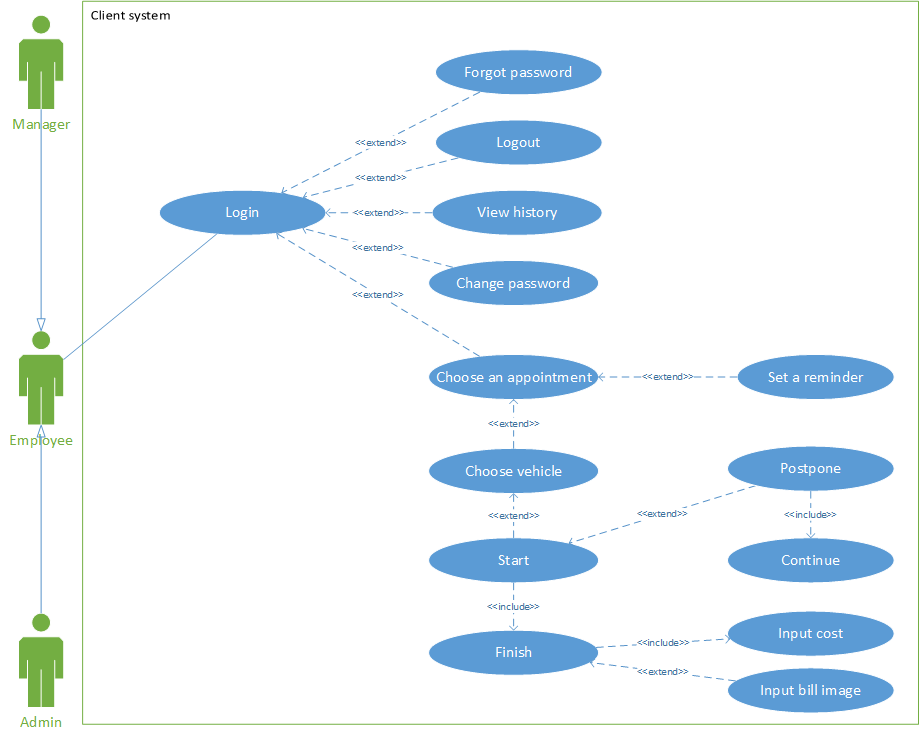
\includegraphics[scale=0.6]{UsecaseDiagram/UseCaseDiagramEmployeeTTTN}
    \centering
    \caption{Lược đồ Use-Case của hệ thống quản lý lịch trình đi lại của nhân viên (dành cho nhân viên)}
    \label{fig:usecase_employee}
\end{figure}
\newpage
\begin{figure}[!h]
    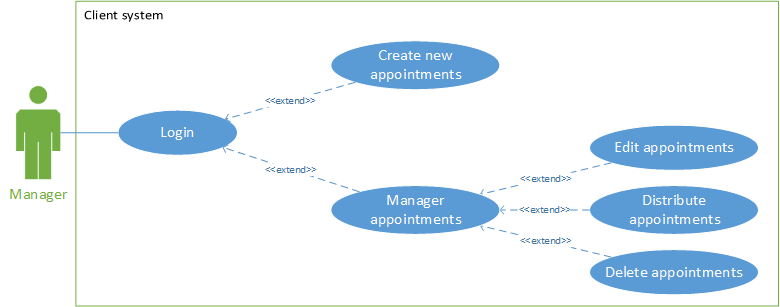
\includegraphics[scale=0.71]{UsecaseDiagram/UsecaseDiagramManagerTTTN}
    \centering
    \caption{Lược đồ Use-Case của hệ thống quản lý lịch trình đi lại của nhân viên (dành cho manager)}
    \label{fig:usecase_manager}
\end{figure}
\begin{figure}[!h]
    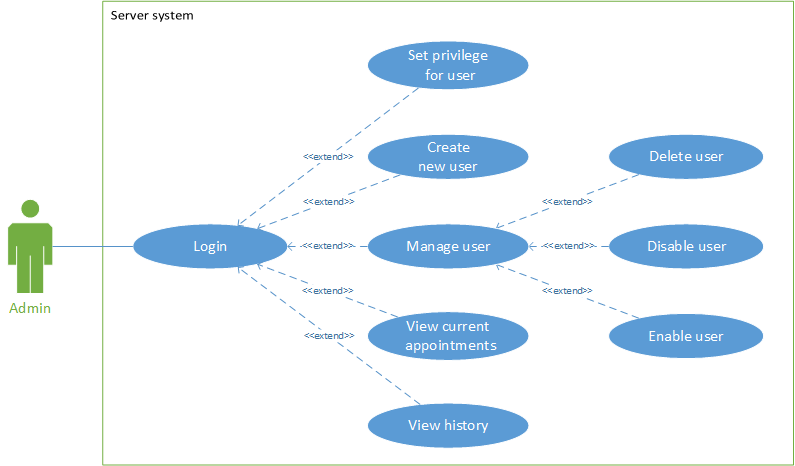
\includegraphics[scale=0.7]{UsecaseDiagram/UseCaseDiagramServerTTTN}
    \centering
    \caption{Lược đồ Use-Case của hệ thống quản lý lịch trình đi lại của nhân viên (dành cho admin)}
    \label{fig:usecase_server}
\end{figure}

\subsubsection{Đặc tả UseCase}
\textbf{Những Use-Case của Admin (Người quản trị hệ thống)}\\
\\
\begin{table}[!h]
    \centering
        \begin{tabular}{|m{3.2cm}|m{10.5cm}|}
        \hline
        Name & Login\\
        \hline
        Summary & Chức năng đăng nhập vào website quản trị dành cho admin\\
        \hline
        Actors & Admin\\
        \hline
        Basic course of Event & -	Admin truy cập vào ứng dụng.\\
                & -	Ứng dụng yêu cầu nhập username và password.\\
                & -	Admin nhập username và password.\\
                & -	Hệ thống kiểm tra username và password hợp lệ.\\
                & -	Hiện thị đăng nhập thành công.
                \\
        \hline
        Exception paths & Admin không thể đăng nhập vào hệ thống, và nhận thông báo lí do\\
        \hline
        Preconditions & Admin phải có tài khoản hợp lệ \\
        \hline
        Post conditions & Admin đăng nhập thành công\\
        \hline
        Business rules & \\
        \hline
        \end{tabular}
        \caption{Đặc tả usecase "Login"}
\end{table}
\clearpage  
\begin{table}[!h]
    \centering
        \begin{tabular}{|m{3.2cm}|m{10.5cm}|}
        \hline
        Name & Create new user’s account\\
        \hline
        Summary & Chức năng tạo và cấp tài khoản cho nhân viên.\\
        \hline
        Actors & Admin\\
        \hline
        Basic course of Event & -	Admin đăng nhập thành công vào hệ thống\\
&-	Admin truy cập vào chức năng Create new user’s account\\
&-	Admin nhập các thông tin cần thiết để tạo tài khoản cho nhân viên\\
        \hline
        Preconditions & Admin phải đăng nhập hệ thống thành công \\
        \hline
        Post conditions &\\
        \hline
        Business rules & \\
        \hline
        \end{tabular}
        \caption{Đặc tả usecase "Create new user’s account"}
\end{table}  
\begin{table}[!h]
    \centering
        \begin{tabular}{|m{3.2cm}|m{10.5cm}|}
        \hline
        Name & Manage User\\
        \hline
        Summary & -	Kích hoạt hoặc vô hiệu tài khoản của nhân viên.\\
&-	Xóa tài khoản không sử dụng của nhân viên.\\
&-	Thay đổi thông tin cần thiết của nhân viên.\\
        \hline
        Actors & Admin\\
        \hline
        Basic course of Event & -	Admin đăng nhập thành công vào hệ thống.\\
&-	Admin truy cập vào chức năng Manage  Account.\\
&-	Admin nhập các thông tin thay đổi để cập nhật.\\
&-	Admin xác nhận kích hoạt hoặc vô tiệu tài khoản.\\
&-	Hệ thống lưu các thông tin vào cơ sở dữ liệu.\\
        \hline
        Preconditions & Admin phải đăng nhập hệ thống thành công \\
        \hline
        Post conditions & Hệ thông lưu các thông tin thay đổi vào cơ sở dữ liệu.\\
        \hline
        Business rules & \\
        \hline
        \end{tabular}
        \caption{Đặc tả usecase "Manage User"}
\end{table}  
\begin{table}[!h]
    \centering
        \begin{tabular}{|m{3.2cm}|m{10.5cm}|}
        \hline
        Name & Set privilege for user\\
        \hline
        Summary & Thiết lập các mức quyền của một tài khoản: admin, user hay manager.\\
        \hline
        Actors & Admin\\
        \hline
        Basic course of Event & -	Admin đăng nhập thành công vào hệ thống.\\
&-	Admin truy cập vào chức năng Manage  Account.\\
&-	Admin nhập  thông tin về quyền của một tài khoản thay đổi.\\
&-	Admin xác nhận lưu thông tin thay đổi.\\
&-	Hệ thống lưu các thông tin vào cơ sở dữ liệu.\\
        \hline
        Preconditions & Admin phải đăng nhập hệ thống thành công. \\
        \hline
        Post conditions & Hệ thông lưu các thông tin thay đổi vào cơ sở dữ liệu.\\
        \hline
        Business rules & \\
        \hline
        \end{tabular}
        \caption{Đặc tả usecase "Set privilege for user"}
\end{table}  
\clearpage
\begin{table}[!h]
    \centering
        \begin{tabular}{|m{3.2cm}|m{10.5cm}|}
        \hline
        Name & View Histoty\\
        \hline
        Summary & -	Hiển thị danh sách các cuộc hẹn trong quá khứ của nhân viên.\\
&-	Hiển thị thống kê địa điểm đến, thời gian, số tiền chi trả, phương tiện di chuyển, con đường đã đi của nhân viên.\\
        \hline
        Actors & Admin\\
        \hline
        Basic course of Event & - Admin đăng nhập thành công vào hệ thống.\\
&-	Admin truy cập vào chức năng View History.\\
&-	Hệ thống hiển thị những thông tin cần thiết.\\
        \hline
        Preconditions & Admin phải đăng nhập hệ thống thành công \\
        \hline
        Post conditions & \\
        \hline
        Business rules & \\
        \hline
        \end{tabular}
        \caption{Đặc tả usecase "View Histoty"}
\end{table}
\begin{table}[!h]
    \centering
        \begin{tabular}{|m{3.2cm}|m{10.5cm}|}
        \hline
        Name & View Current Appointments\\
        \hline
        Summary & -	Hiển thị danh sách các cuộc hẹn hiện có của nhân viên.\\
&-	Hiển thị địa điểm đến, thời gian, phương tiện di chuyển, con đường đề xuất cho nhân viên.\\
        \hline
        Actors & Admin\\
        \hline
        Basic course of Event & -	Admin đăng nhập thành công vào hệ thống.\\
&-	Admin truy cập vào chức năng View Current Appointments.\\
&-	Hệ thống hiển thị những thông tin cần thiết.\\
        \hline
        Preconditions & Admin phải đăng nhập hệ thống thành công. \\
        \hline
        Post conditions & \\
        \hline
        Business rules & \\
        \hline
        \end{tabular}
        \caption{Đặc tả usecase "View Current Appointments"}
\end{table}
\noindent
\textbf{Những Use-Case của Employee:}\\
\begin{table}[!h]
    \centering
    \begin{tabular}{|m{3.2cm}|m{10.5cm}|}
        \hline
        Name & Login\\
        \hline
        Summary & Chức năng đăng nhập vào ứng dụng.\\
        \hline
        Actors & Employee\\
        \hline
        Basic course of Event & -	Người dùng truy cập vào ứng dụng.\\
&-	Ứng dụng yêu cầu nhập username và password.\\
&-	Người dùng nhập username và password.\\
&-	Hệ thống kiểm tra username và password hợp lệ.\\
&-	Hiển thị đăng nhập thành công.\\
        \hline
        Exception paths & Người dùng không thể đăng nhập vào hệ thống, và nhận thông báo lí do.\\
        \hline
        Preconditions & Người dùng phải có tài khoản hợp lệ do admin cấp.\\
        \hline
        Post conditions & Người dùng đăng nhập thành công.\\
        \hline
        Business rules & \\
        \hline
    \end{tabular}
    \caption{Đặc tả usecase "Login"}
\end{table}
\begin{table}[!h]
    \centering
    \begin{tabular}{|m{3.2cm}|m{10.5cm}|}
        \hline
        Name & Forgot password\\
        \hline
        Summary & Chức năng yêu cầu lấy lại mật khẩu.\\
        \hline
        Actors & Employee\\
        \hline
        Basic course of Event & -	User yêu cầu lấy lại mật khẩu.\\
&-	Hệ thống yêu cầu thiết lập mật khẩu mới gửi tới email cho người dùng.\\
        \hline
        Preconditions & Người dùng phải có tài khoản tồn tại trong hệ thống.\\
        \hline
        Post conditions & Người dùng đăng nhập thành công.\\
        \hline
        Business rules & \\
        \hline
    \end{tabular}
    \caption{Đặc tả usecase "Forgot password"}
\end{table}
\begin{table}[!h]
    \centering
    \begin{tabular}{|m{3.2cm}|m{10.5cm}|}
        \hline
        Name & Change password\\
        \hline
        Summary & Chức năng đổi mật khẩu tài khoản.\\
        \hline
        Actors & Employee\\
        \hline
        Basic course of Event & -	User chọn chức năng Change password.\\
&-	User nhập những thông tin cần thiết như current password, new password, confirm password…\\
&-	Hệ thống kiểm tra và cập nhật.\\
        \hline
        Preconditions & Người dùng đăng nhập vào ứng dụng thành công.\\
        \hline
        Post conditions & Hệ thống cập nhật mật khẩu mới của tài khoản người dùng.\\
        \hline
        Business rules & \\
        \hline
    \end{tabular}
    \caption{Đặc tả usecase "Change password"}
\end{table}
\begin{table}[!h]
    \centering
    \begin{tabular}{|m{3.2cm}|m{10.5cm}|}
        \hline
        Name & View Histoty\\
        \hline
        Summary & -	Hiển thị danh sách các cuộc hẹn trong quá khứ của bản thân người dùng.\\
&-	Hiển thị thống kê địa điểm đến, thời gian, số tiền chi trả, phương tiện di chuyển, con đường đã đi của bản thân người dùng.\\
        \hline
        Actors & Employee\\
        \hline
        Basic course of Event & -	Admin đăng nhập thành công vào ứng dụng.\\
&-	Admin truy cập vào chức năng View History.\\
&-	Hệ thống hiển thị những thông tin cần thiết.\\
        \hline
        Preconditions & Người dùng  phải đăng nhập hệ thống thành công.\\
        \hline
        Post conditions & \\
        \hline
        Business rules & \\
        \hline
    \end{tabular}
    \caption{Đặc tả usecase "View Histoty"}
\end{table}
\begin{table}[!h]
    \centering
    \begin{tabular}{|m{3.2cm}|m{10.5cm}|}
        \hline
        Name & Choose appointment\\
        \hline
        Summary & -	Người dùng xem danh sách các cuộc hẹn hiện có.\\
&-	Người dùng chọn một cuộc hẹn trong danh sách để tương tác.\\
        \hline
        Actors & Employee\\
        \hline
        Basic course of Event & -	Người dùng đăng nhập thành công vào ứng dụng.\\
&-	Người dùng truy cập vào chức năng xem danh sách cuộc hẹn.\\
&-	Người dùng chọn một cuộc hẹn để thực hiện hoặc thiết lập nhắc nhở. \\
        \hline
        Preconditions & Người dùng  phải đăng nhập hệ thống thành công\\
        \hline
        Post conditions & \\
        \hline
        Business rules & \\
        \hline
    \end{tabular}
    \caption{Đặc tả usecase "Choose appointment"}
\end{table}
\begin{table}[!h]
    \centering
    \begin{tabular}{|m{3.2cm}|m{10.5cm}|}
        \hline
        Name & Set a reminder\\
        \hline
        Summary & Người dùng chọn một cuộc hẹn trong danh sách để thiết lập nhắc nhở thời gian thông báo.\\
        \hline
        Actors & Employee\\
        \hline
        Basic course of Event & -	Người dùng đăng nhập thành công vào ứng dụng.\\
&-	Người dùng chọn một cuộc hẹn.\\
&-	Người dùng thiết lập thời gian sẽ nhắc nhở đối với cuộc hẹn đã chọn.\\
        \hline
        Preconditions & -	Người dùng  phải đăng nhập hệ thống thành công.\\
&-	Người dùng đã chọn một cuộc hẹn.\\
        \hline
        Post conditions &\\
        \hline
        Business rules & \\
        \hline
    \end{tabular}
    \caption{Đặc tả usecase "Set a reminder"}
\end{table}
\begin{table}[!h]
    \centering
    \begin{tabular}{|m{3.2cm}|m{10.5cm}|}
        \hline
        Name & Choose a vehicle\\
        \hline
        Summary & Chức năng chọn phương tiện.\\
        \hline
        Actors & Employee\\
        \hline
        Basic course of Event & -	Người dùng đăng nhập thành công vào ứng dụng.\\
&-	Người dùng chọn một cuộc hẹn.\\
&-	Người dùng chọn phương tiện đối với cuộc hẹn muốn thực hiện.\\
        \hline
        Preconditions & -	Người dùng  phải đăng nhập hệ thống thành công.\\
&-	Người dùng đã chọn một cuộc hẹn.\\
        \hline
        Post conditions & \\
        \hline
        Business rules & \\
        \hline
    \end{tabular}
    \caption{Đặc tả usecase "Choose a vehicle"}
\end{table}
\begin{table}[!h]
    \centering
    \begin{tabular}{|m{3.2cm}|m{10.5cm}|}
        \hline
        Name & Start \\
        \hline
        Summary & Bắt đầu thực hiện cuộc hẹn đã chọn sau khi đã chọn phương tiện.\\
        \hline
        Actors & Employee\\
        \hline
        Basic course of Event & -	Người dùng đăng nhập thành công vào ứng dụng.\\
&-	Người dùng chọn một cuộc hẹn và chọn phương tiện.\\
&-	Người dùng bắt đầu thực hiện cuộc hẹn, hệ thống có thể đề xuất con đường phù hợp ban đầu.\\
        \hline
        Preconditions & -	Người dùng  phải đăng nhập hệ thống thành công.\\
&-	Người dùng đã chọn một cuộc hẹn và chọn phương tiện.\\
        \hline
        Post conditions & \\
        \hline
        Business rules & \\
        \hline
    \end{tabular}
    \caption{Đặc tả usecase "Start"}
\end{table}
\begin{table}[!h]
    \centering
    \begin{tabular}{|m{3.2cm}|m{10.5cm}|}
        \hline
        Name & Postpone\\
        \hline
        Summary & Tạm hoãn một cuộc hẹn đang thực hiện vì công việc đột xuất hoặc chuyển phương tiện.\\
        \hline
        Actors & Employee\\
        \hline
        Basic course of Event & -	Người dùng đăng nhập thành công vào ứng dụng.\\
&-	Người dùng bắt đầu thực hiện một cuộc hẹn.\\
&-	Người dùng tạm hoãn lại cuộc hẹn đang thực hiện.\\
        \hline
        Preconditions &-	Người dùng  phải đăng nhập hệ thống thành công.\\
&-	Người dùng đã chọn một cuộc hẹn và đang thực hiện nó.\\
        \hline
        Post conditions &\\
        \hline
        Business rules & \\
        \hline
    \end{tabular}
    \caption{Đặc tả usecase "Postpone"}
\end{table}
\begin{table}[!h]
    \centering
    \begin{tabular}{|m{3.2cm}|m{10.5cm}|}
        \hline
        Name & Continue\\
        \hline
        Summary & Tiếp tục thực hiện một cuộc hẹn sau khi tạm hoãn.\\
        \hline
        Actors & Employee\\
        \hline
        Basic course of Event & -	Người dùng đăng nhập thành công vào ứng dụng.\\
&-	Người dùng đang tạm hoãn đối với một cuộc hẹn.\\
&-	Người dùng tiếp tục thực hiện nó sau khi tạm hoãn.\\
        \hline
        Preconditions & -	Người dùng  phải đăng nhập hệ thống thành công.\\
&-	Người dùng đang thực hiện cuộc hẹn và tạm hoãn.\\
        \hline
        Post conditions & \\
        \hline
        Business rules & \\
        \hline
    \end{tabular}
    \caption{Đặc tả usecase "Continue"}
\end{table}
\begin{table}[!h]
    \centering
    \begin{tabular}{|m{3.2cm}|m{10.5cm}|}
        \hline
        Name & Finish \\
        \hline
        Summary & Đánh dấu đã đến địa điểm hẹn, kết thúc một cuộc hẹn.\\
        \hline
        Actors & Employee\\
        \hline
        Basic course of Event & -	Người dùng chọn vào tính năng Finish, kết thúc một cuộc hẹn.\\
&-	Người dùng nhập chi phí đi lại, và hóa đơn (nếu có).\\
        \hline
        Preconditions &-	Người dùng  phải đăng nhập hệ thống thành công.\\
&-	Người dùng phải đang thực hiện Start.\\
        \hline
        Post conditions & Hệ thống tính toán và dự đoán chi phí đi lại, để xác thực với chi phí mà người dùng nhập vào.\\
        \hline
        Business rules & \\
        \hline
    \end{tabular}
    \caption{Đặc tả usecase "Finish"}
\end{table}
\begin{table}[!h]
    \centering
    \begin{tabular}{|m{3.2cm}|m{10.5cm}|}
        \hline
        Name & Input cost\\
        \hline
        Summary & Chức năng nhập chi phí đi lại.\\
        \hline
        Actors & Employee\\
        \hline
        Basic course of Event & -	Người dùng chọn vào tính năng Finish, kết thúc một cuộc hẹn hoặc chuyện đổi phương tiện.\\
&-	Người dùng nhập chi phí đi lại đối với loại phương tiện đó.\\
        \hline
        Preconditions & -	Người dùng  phải đăng nhập hệ thống thành công.\\
&-	Người dùng đã chọn Finish hoặc chuyển đổi phương tiện.\\
        \hline
        Post conditions & Hệ thống lưu lại chi phí đã nhập và dự đoán chi phí trong hệ thống.\\
        \hline
        Business rules & \\
        \hline
    \end{tabular}
    \caption{Đặc tả usecase "Input cost"}
\end{table}
\begin{table}[!h]
    \centering
    \begin{tabular}{|m{3.2cm}|m{10.5cm}|}
        \hline
        Name & Input bill image\\
        \hline
        Summary & Chức năng nhập hình ảnh hóa đơn\\
        \hline
        Actors & Employee\\
        \hline
        Basic course of Event & -	Người dùng chọn vào tính năng Finish, kết thúc một cuộc hẹn hoặc chuyện đổi phương tiện.\\
&-	Người dùng chụp và gửi hình ảnh hóa đơn nếu có.\\
        \hline
        Preconditions &-	Người dùng  phải đăng nhập hệ thống thành công.\\
&-	Người dùng đã chọn Finish hoặc chuyển đổi phương tiện.\\
        \hline
        Post conditions & Hệ thống lưu lại hình ảnh hóa đơn.\\
        \hline
        Business rules & \\
        \hline
    \end{tabular}
    \caption{Đặc tả usecase "Input bill image"}
\end{table}
\clearpage
\noindent
\textbf{Những Use-Case của Manager:}\\
\begin{table}[!h]
    \centering
    \begin{tabular}{|m{3.2cm}|m{10.5cm}|}
        \hline
        Name & Create new appointments\\
        \hline
        Summary & Chức năng tạo một cuộc hẹn với khách hàng.\\
        \hline
        Actors & Manager\\
        \hline
        Basic course of Event & Manager tạo một địa điểm và thời gian của một cuộc hẹn.\\
        \hline
        Preconditions &Người dùng đăng nhập thành công vào hệ thống.\\
        \hline
        Post conditions & \\
        \hline
        Business rules & \\
        \hline
    \end{tabular}
    \caption{Đặc tả usecase "Create new appointments"}
\end{table}
\begin{table}[!h]
    \centering
    \begin{tabular}{|m{3.2cm}|m{10.5cm}|}
        \hline
        Name & Edit appointments\\
        \hline
        Summary & Chức năng chỉnh sửa một cuộc hẹn với khách hàng.\\
        \hline
        Actors & Manager\\
        \hline
        Basic course of Event & Manager chỉnh sửa địa điểm và thời gian của một cuộc hẹn.\\
        \hline
        Preconditions &-	Manager đăng nhập thành công vào hệ thống.\\
&-	Manager đã tạo một cuộc hẹn trước đó.\\
        \hline
        Post conditions & \\
        \hline
        Business rules & \\
        \hline
    \end{tabular}
    \caption{Đặc tả usecase "Edit appointments"}
\end{table}
\begin{table}[!h]
    \centering
    \begin{tabular}{|m{3.2cm}|m{10.5cm}|}
        \hline
        Name & Delete appointments\\
        \hline
        Summary & Xóa một cuộc hẹn với khách hàng.\\
        \hline
        Actors & Manager\\
        \hline
        Basic course of Event & Manager xóa cuộc hẹn.\\
        \hline
        Preconditions &-	Manager đăng nhập thành công vào hệ thống.\\
&-	Manager đã tạo một cuộc hẹn trước đó.\\
        \hline
        Post conditions & \\
        \hline
        Business rules & \\
        \hline
    \end{tabular}
    \caption{Đặc tả usecase "Delete appointments"}
\end{table}
\begin{table}[!h]
    \centering
    \begin{tabular}{|m{3.2cm}|m{10.5cm}|}
        \hline
        Name & Distribute appointments\\
        \hline
        Summary & Gán một cuộc hẹn với khách hàng cho nhân viên.\\
        \hline
        Actors & Manager\\
        \hline
        Basic course of Event & Manager sắp xếp một cuộc hẹn cho một nhân viên.\\
        \hline
        Preconditions &-	Manager đăng nhập thành công vào hệ thống.\\
&-	Manager đã tạo một cuộc hẹn trước đó.\\
        \hline
        Post conditions & \\
        \hline
        Business rules & \\
        \hline
    \end{tabular}
    \caption{Đặc tả usecase "Distribute appointments"}
\end{table}
\newpage
\section{Thiết kế}
\subsection{Thiết kế hệ thống}
\begin{figure}[h]
    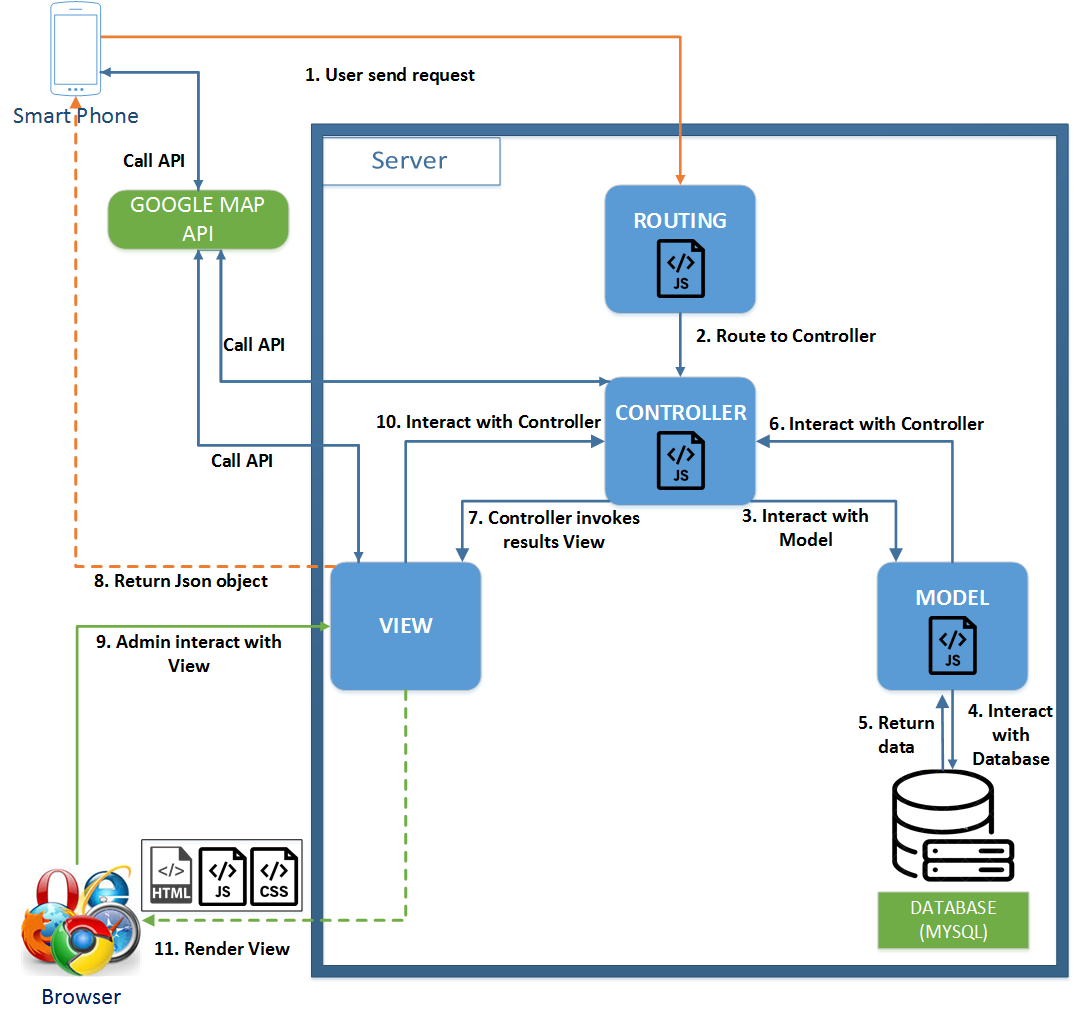
\includegraphics[scale=0.5]{architecture}
    \centering
    \caption{Kiến trúc tổng quát của hệ thống}
    \label{fig:architecture}
\end{figure}
\noindent
Kiến trúc hệ thống nhóm thiết kế sẽ dựa theo mô hình MVC. Client và Server sẽ giao tiếp qua giao thức HTTP, sử dụng cấu trúc file JSON vì một số ưu điểm của nó so với cấu trúc file XML.\\
\\
Người dùng trong hệ thống bao gồm có nhân viên, quản lý và người quản trị hệ  thống. Người dùng truy cập vào hệ thống thông qua các thiết bị di động và thiết bị trình duyệt brower.\\
\\
Qua khảo sát, nhóm quyết định chọn Java để hiện thực Server vì nhóm đã từng sử dụng và có kinh nghiệm về nó hơn các công nghệ hiện thực Server khác. Mặt khác nhóm cảm thấy Java có nhiều ưu điểm phù hợp để xây dựng một Server như : Hiệu suât cao khi hệ thống phát triển lớn, các tiến trình đơn giản nhưng hiệu năng cao, không đệm.\\\\
Framework nhóm sử dụng để hỗ trợ việc xây dựng Server là Spring Franework. Một số ưu điểm nổi bật của nó như là : hỗ trợ REST API, định nghĩa routes và các request method đến Server một cách dễ dàng.\\
\\
Luồng chạy tổng quát của hệ thống:\\
\\
\textbf{Đối với người dùng là nhân viên, quản lý:} Khi người dùng gửi yêu cầu lên Server thông qua thiết bị di động, Server sẽ chuyển yêu cầu này cho thành phần định tuyến (1) \textit{(Routing)}. Routing sẽ chuyển những yêu cầu này đến Controller tương ứng (2) \textit{(bộ điều khiển đồng bộ hóa giữa View và Model)} dựa trên địa chỉ URL được cung cấp. Một số Controller trong hệ thống như \textit{ControllerEmployee, ControllerManager, ControllerAppointment}... Controller sẽ tương tác với Model (3) \textit{(đây là thành phần chứa các nghiệp vụ logic, phương thức xử lý, truy xuất database, đối tượng mô tả dữ liệu như các class, hàm xử lý,...)}. Model tương tác với Database (4), sau đó Database trả kết quả về cho Model (5), Model trả kết quả về cho Controller (6). Cuối cùng Controller sẽ trả về kết quả cho Client dưới dạng cấu trúc file JSON.\\
\\
\textbf{Đối với người dùng là admin:} Người dùng sẽ tương tác với thành phần View (9), thành phần View sẽ chuyển yêu cầu này đến cho Controller tương ứng để xử lý tác vụ (10). Sau đó Controller sẽ tương tác với Model (3). Model tương tác với Database (4), sau đó Database trả kết quả về cho Model (5), Model trả kết quả về cho Controller (6). Cuối cùng Controller sẽ tạo nên một View để trả về trình duyệt web (11).\\
\begin{figure}[!h]
    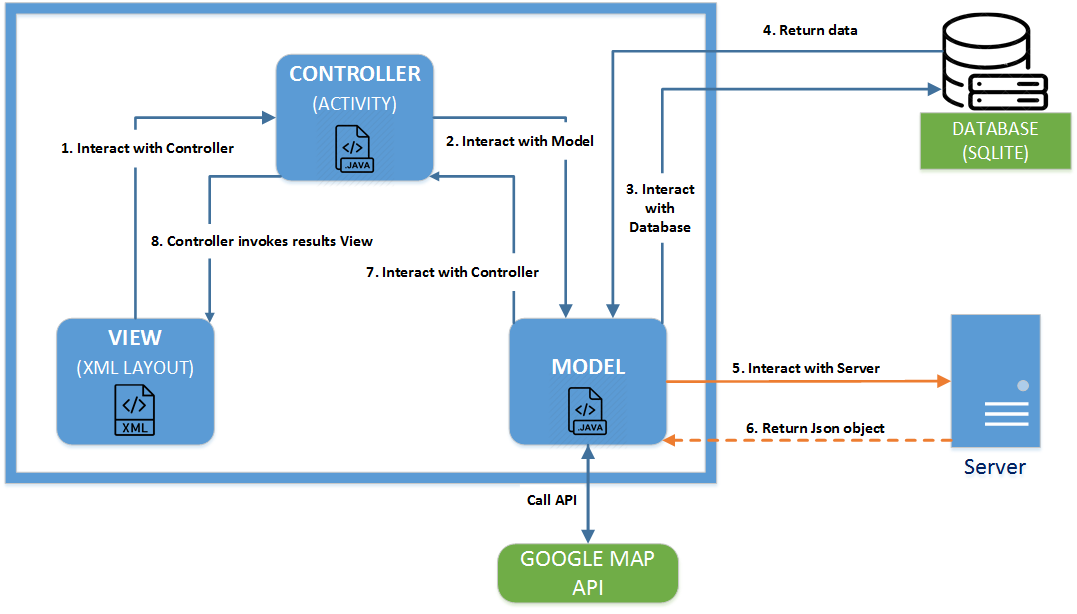
\includegraphics[scale=0.53]{mobile_architecture}
    \centering
    \caption{Kiến trúc thiết bị di động}
    \label{fig:mobile_architecture}
\end{figure}
\clearpage
\noindent
Đối với thiết bị di động nhóm cũng thiết kế dựa theo mô hình MVC.\\
\\
Người dùng sẽ tương tác với thành phần View của thiết bị di động, thành phần View sẽ chuyển yêu cầu này đến cho Controller tương ứng để xử lý tác vụ (1). Sau đó Controller sẽ tương tác với thành phần Model (2). Model có thể tương tác với Database (3)(4) (Cơ sở dữ liệu cục bộ) để cập nhật dữ liệu mới từ Server hoặc truy xuất dữ liệu cục bộ đã có. Ngoài ra Model còn tương tác với Server (5)(6) để cập nhật dữ liệu và gọi Google MAP API để hiện thị và cập nhật quãng đường di chuyển của nhân viên trên View. Model trả kết quả về cho Controller (7). Cuối cùng Controller sẽ cập nhật lại View cho thiết bị di động (8).
%%%%%%%%%%%%%%%%%%%%%%%%%%%%%%%%%%%
%%%%%%%%%%%%%%%%%%%%%%%%%%%%%%%%%%%
\subsection{Thiết kế cơ sở dữ liệu}
\subsubsection{Mô hình thực thể quan hệ - ERD}
Các thực thể trong mô hình ERD ở hình \ref{fig:erd}:
\begin{itemize}
    \item \textbf{EMPLOYEE} đại diện cho loại user nhân viên trong hệ thống. 
\item \textbf{MANAGER} đại diện cho loại user manager trong hệ thống.
\item \textbf{ADMIN} đại diện cho người quản trị trong hệ thống.
\item \textbf{APPOINTMENT} đại diện cho những cuộc hẹn với khách hàng hiện tại đã được tạo.
\item \textbf{DETAIL} đại diện cho quảng đường mà người dùng đi được đối với một loại phương tiện.
\item \textbf{VEHICLE} đại diện cho loại phương tiện mà người dùng sẽ lựa chọn để đi.
\item \textbf{COORDINATES} đại diện cho tọa độ của người dùng trên bản đồ google maps.
\end{itemize}
\begin{sidewaysfigure}
    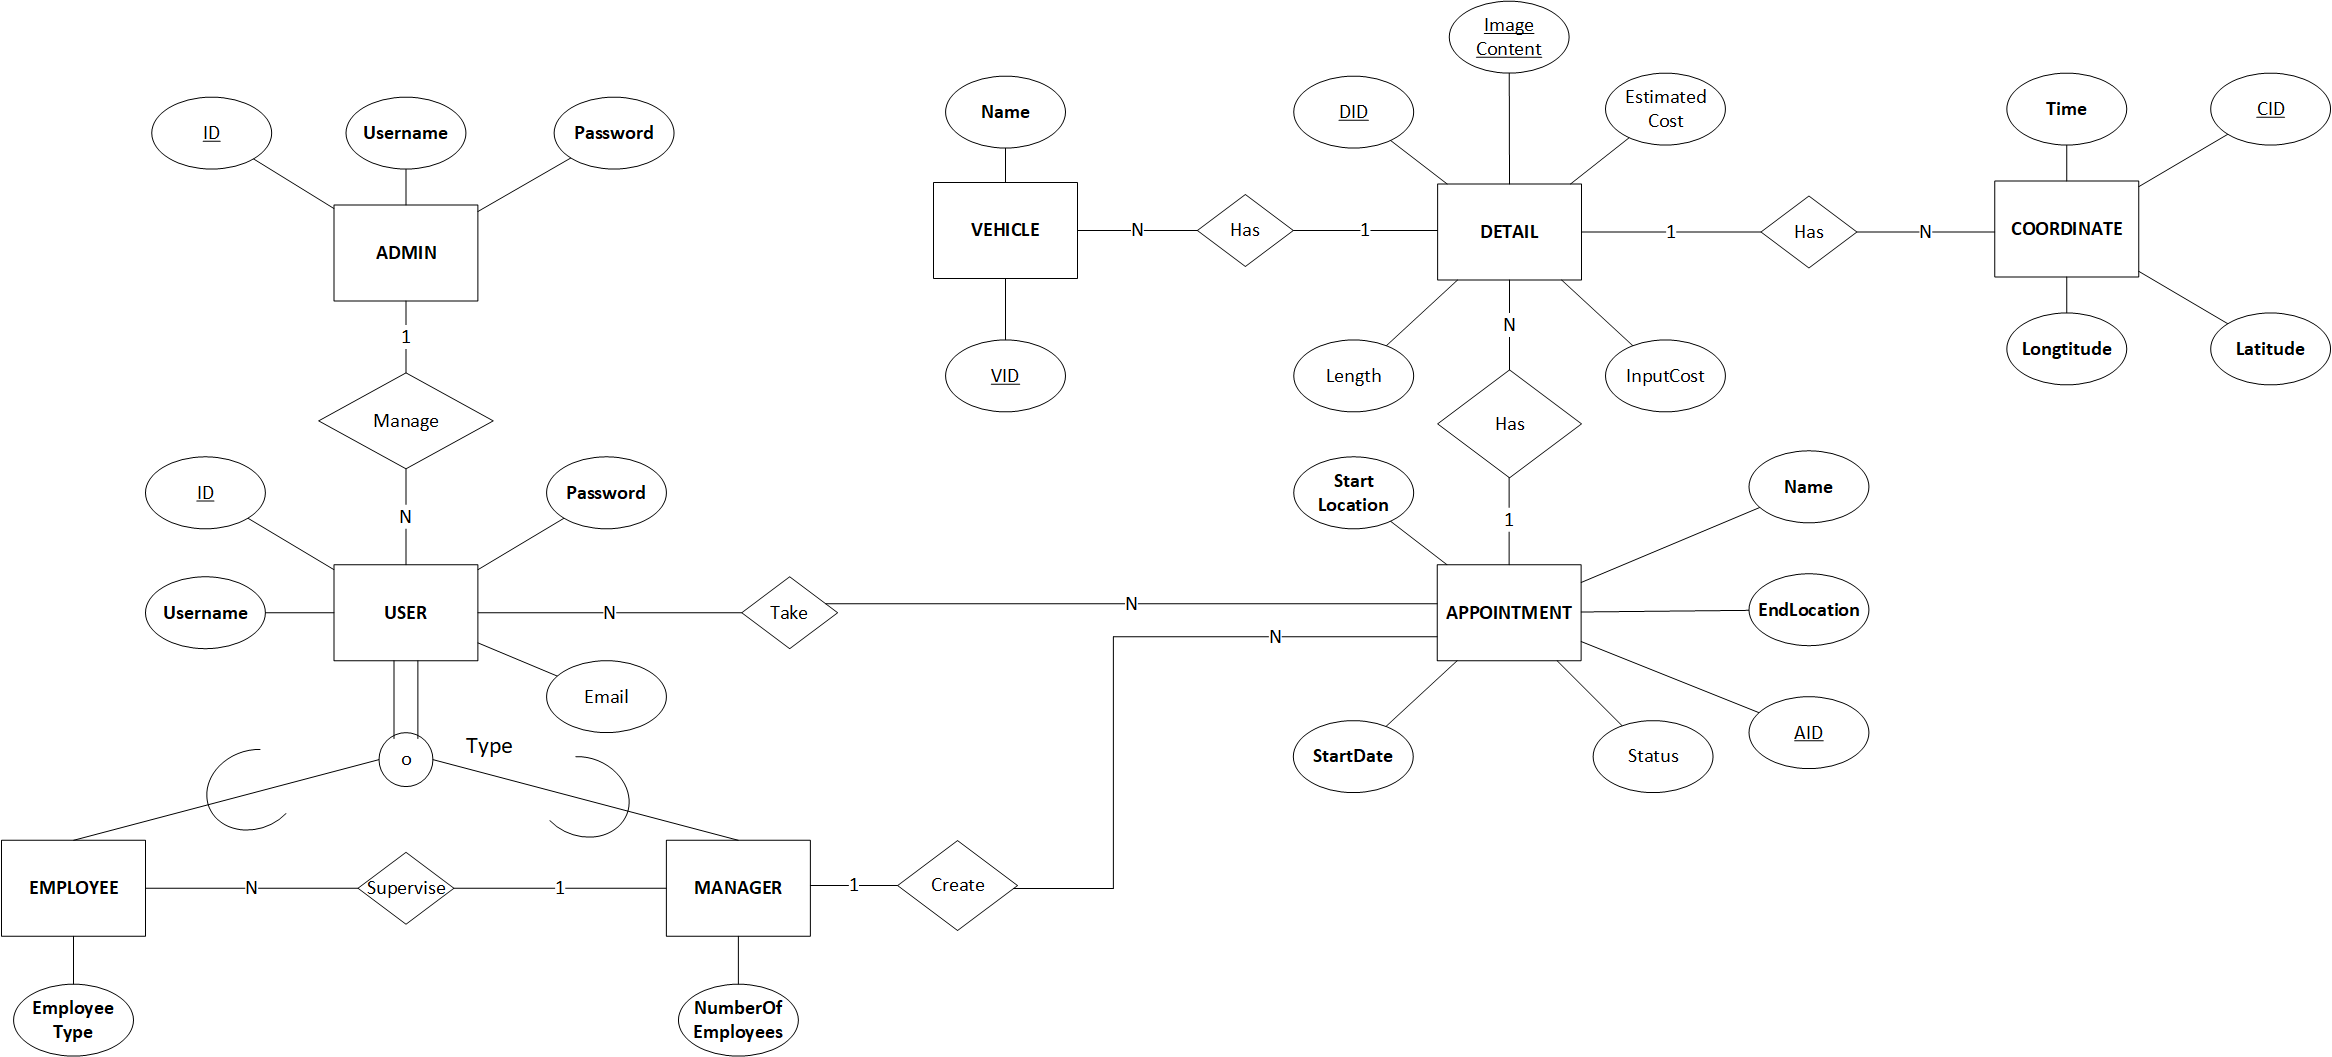
\includegraphics[width=21cm]{erd}
    \caption{Mô hình thực thể quan hệ}
    \label{fig:erd}
\end{sidewaysfigure}
\subsubsection{Ánh xạ mô hình thực thể quan hệ}
Ánh xạ mô hình thực thể quan hệ được thể hiện ở hình \ref{fig:erd2}
\begin{sidewaysfigure}
    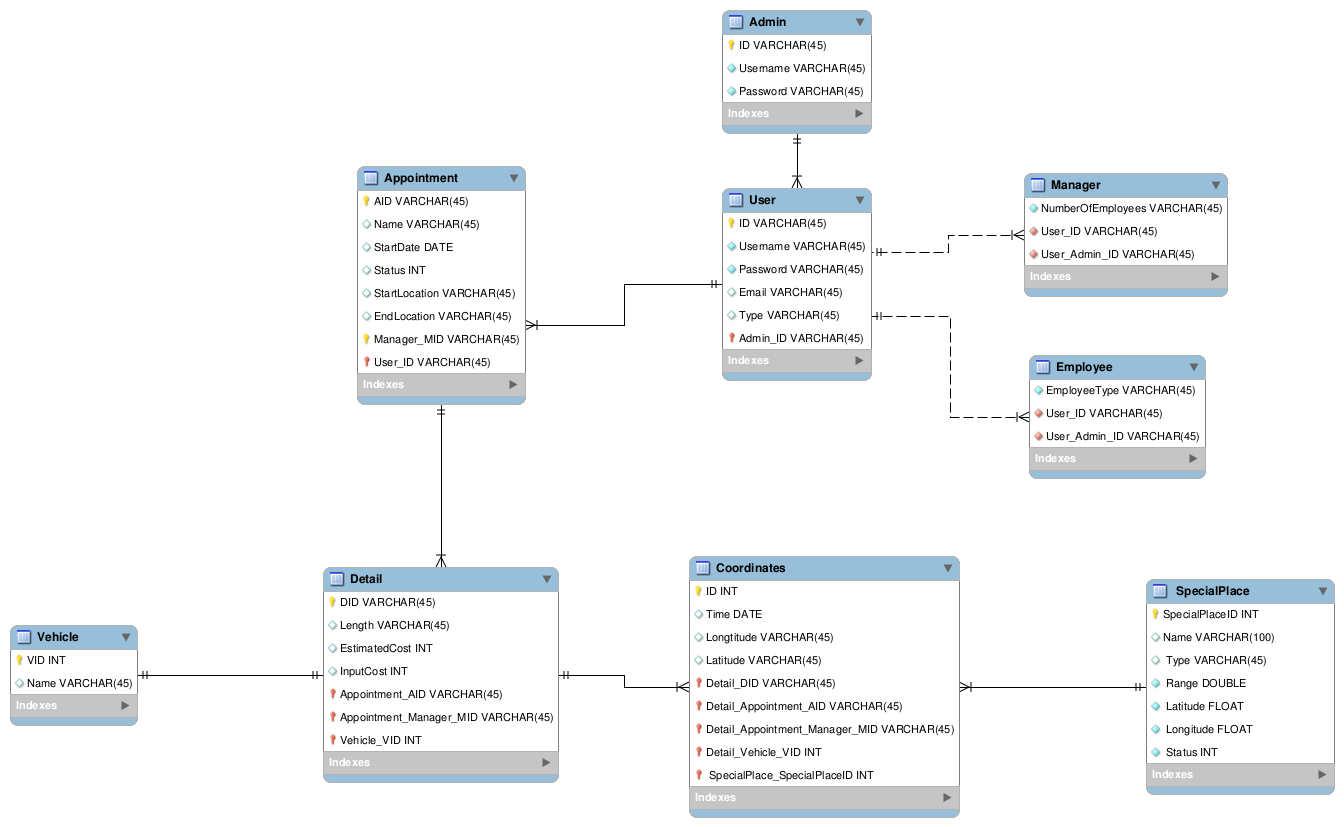
\includegraphics[scale=0.45]{erd2}
    \caption{Ánh xạ mô hình thực thể quan hệ}
    \label{fig:erd2}
\end{sidewaysfigure}
\clearpage
\subsection{Thiết kế giao diện}
Gồm 10 hình thiết kế giao diện cho các màn hình chính  của ứng dụng trên mobile:
\begin{itemize}
    \item Màn hình đăng nhập
    \item Màn hình thông tin user
    \item Màn hình chức năng đổi mật khẩu
    \item Màn hình tạo một điểm hẹn
    \item Màn hình chính, danh sách các điểm hẹn
    \item Màn hình chi tiết của một điểm hẹn
    \item Màn hình hẹn giờ thông báo một điểm hẹn
    \item Màn hình yêu cầu đính kèm minh chứng và nhập số tiền chi trả
    \item Màn hình lịch sử các điểm hẹn    
    \item Màn hình xem lại chi tiết điểm hẹn trong quá khứ
\end{itemize}
\begin{figure}[h]
    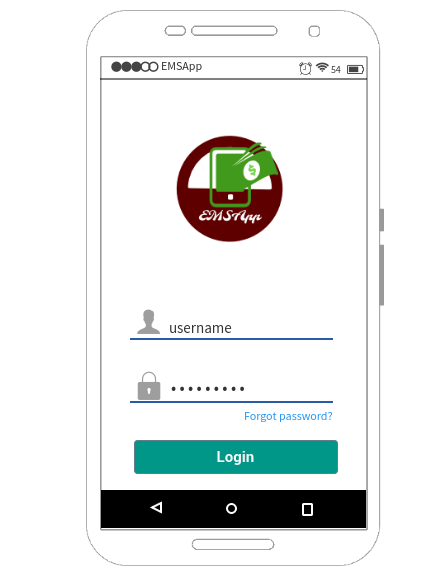
\includegraphics[scale=1]{Mockup/Login}
    \centering
    \caption{Màn hình đăng nhập}
    \label{fig:login}
\end{figure}
\begin{figure}[h]
    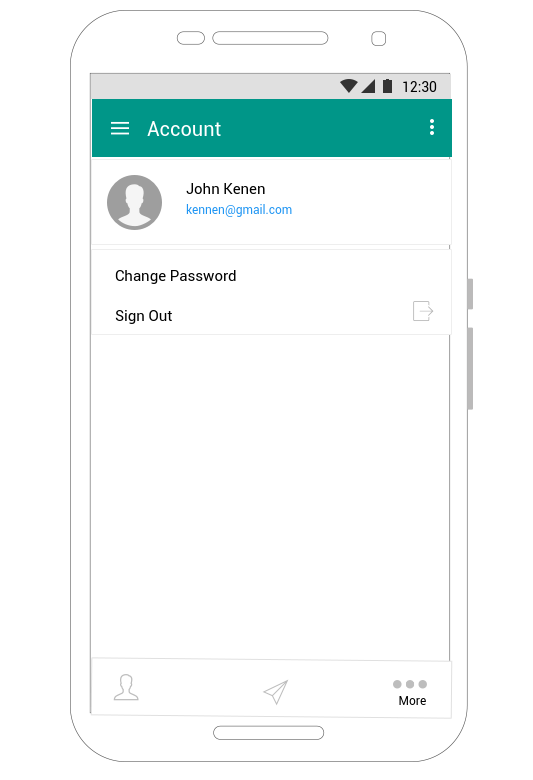
\includegraphics[scale=0.6]{Mockup/AC_user}
    \centering
    \caption{Màn hình thông tin user}
    \label{fig:AC_user}
\end{figure}
\begin{figure}[h]
    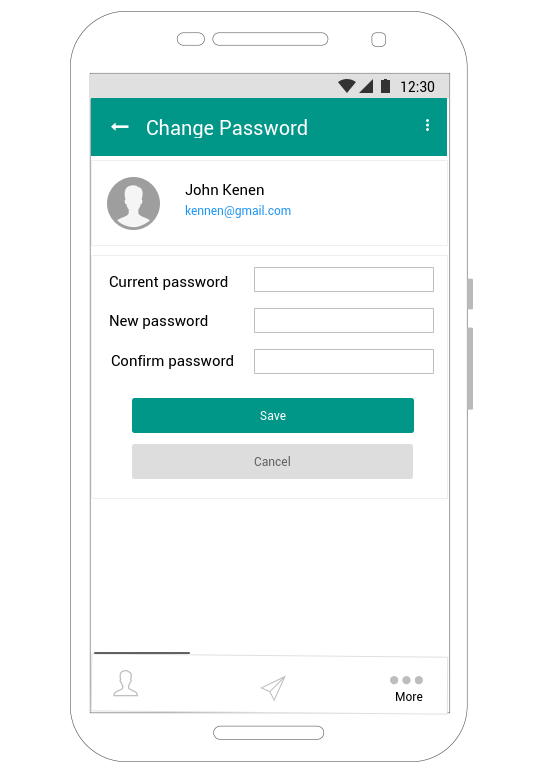
\includegraphics[scale=0.6]{Mockup/AC_changepassword}
    \centering
    \caption{Màn hình chức năng đổi mật khẩu}
    \label{fig:AC_changepassword}
\end{figure}
\begin{figure}[h]
    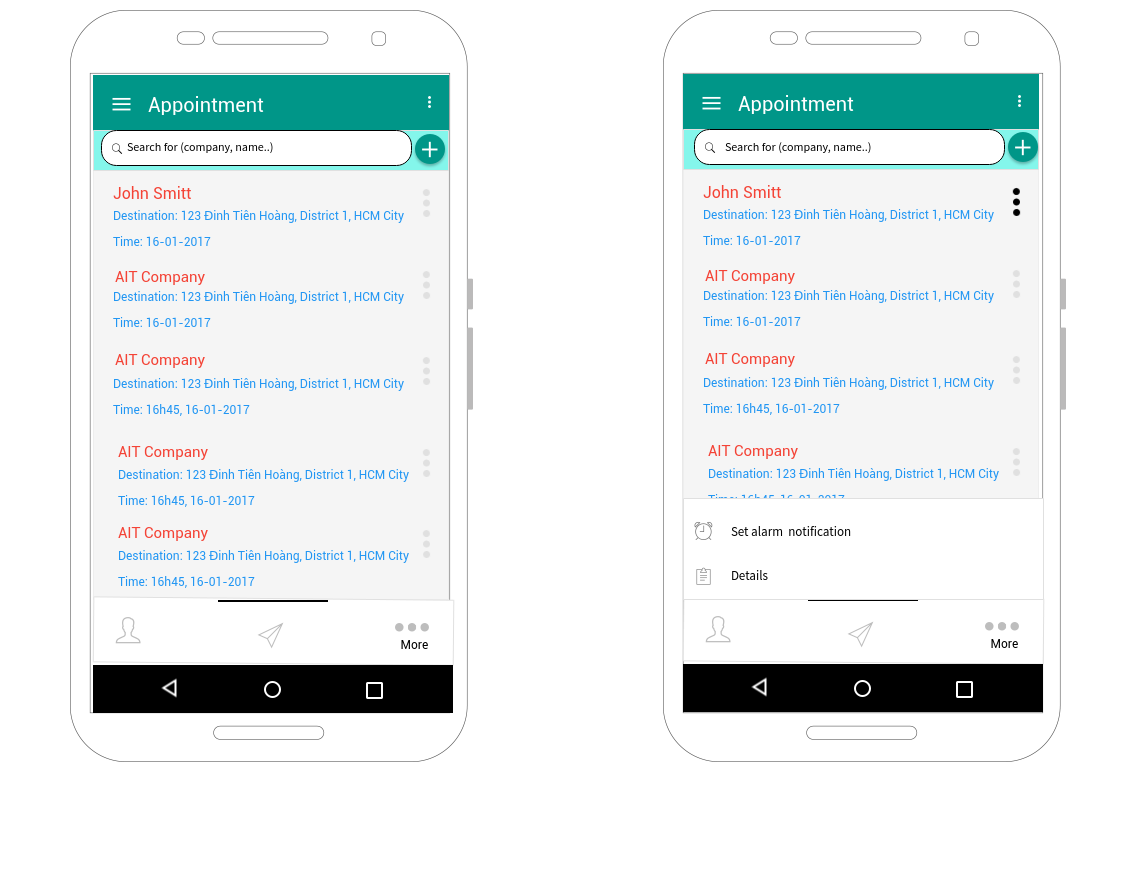
\includegraphics[width=12cm]{Mockup/AP_mainappointment}
    \centering
    \caption{Màn hình chính, danh sách các điểm hẹn}
    \label{fig:AP_mainappointment}
\end{figure}
\begin{figure}[h]
    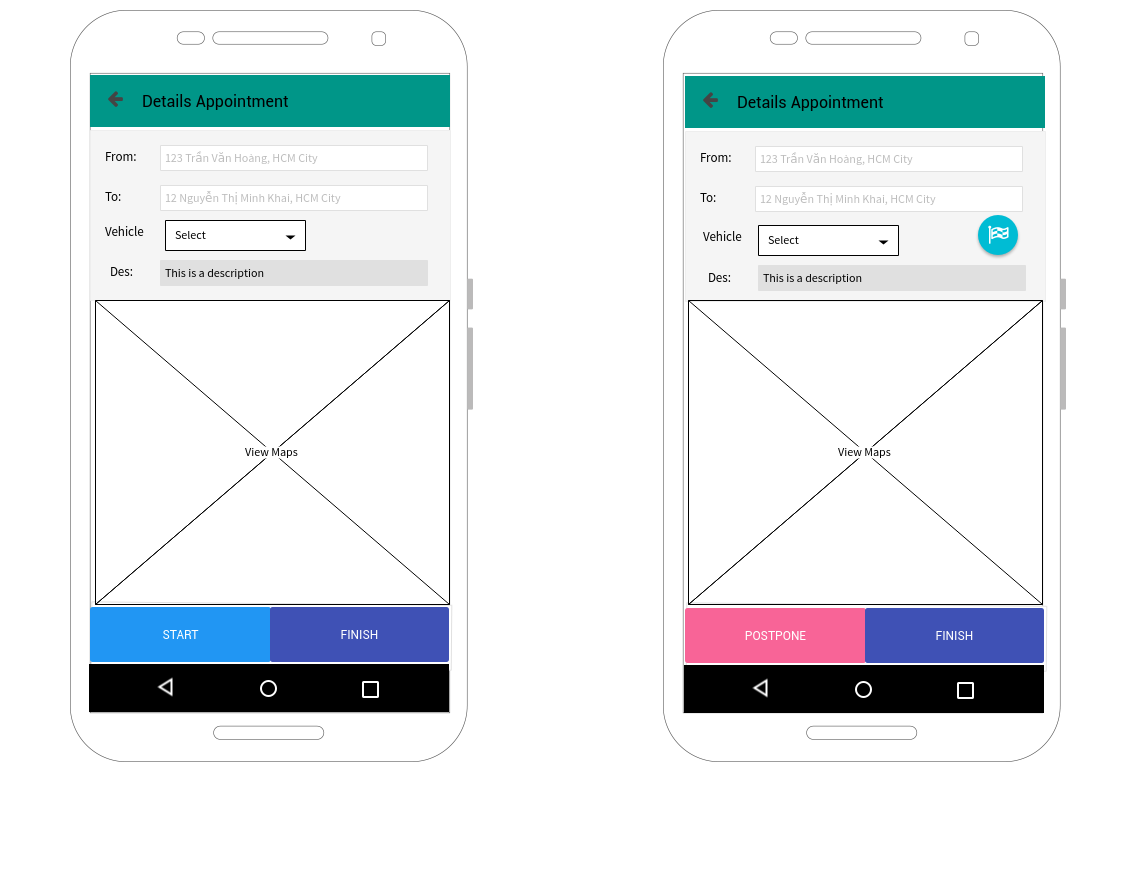
\includegraphics[width=12cm]{Mockup/AP_detailsappointment}
    \centering
    \caption{Màn hình chi tiết một điểm hẹn}
    \label{fig:AP_detailsappointment}
\end{figure}
\begin{figure}[h]
    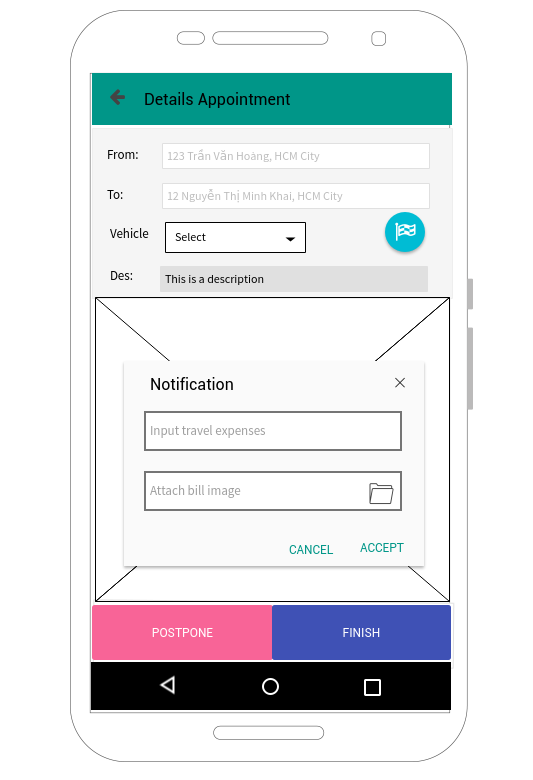
\includegraphics[scale=0.6]{Mockup/AP_finishappointment}
    \centering
    \caption{Màn hình đính kèm minh chứng và nhập số tiền chi trả}
    \label{fig:AP_finishappointment}
\end{figure}
\begin{figure}[h]
    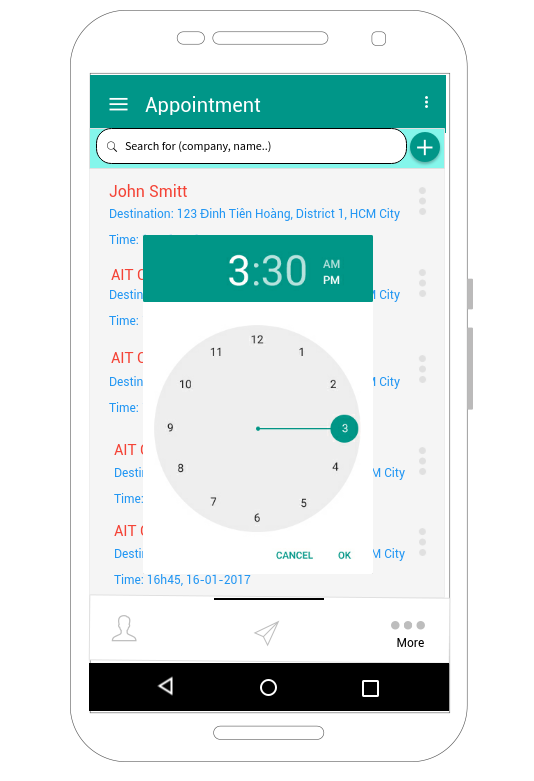
\includegraphics[scale=0.6]{Mockup/AP_picktimeappointment}
    \centering
    \caption{Màn hình hẹn giờ thông báo điểm hẹn}
    \label{fig:AP_picktimeappointment}
\end{figure}
\begin{figure}[h]
    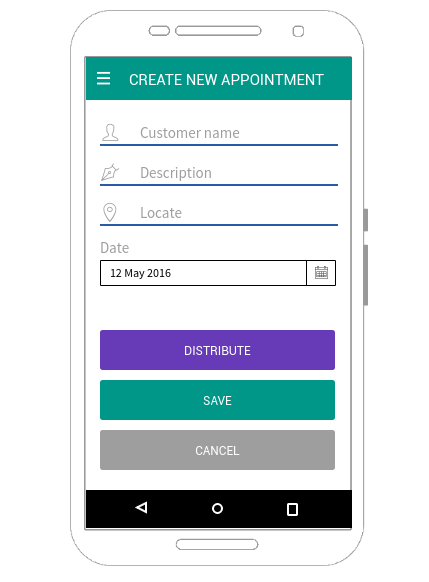
\includegraphics[scale=0.82]{Mockup/AP_newappointment}
    \centering
    \caption{Màn hình tạo một điểm hẹn}
    \label{fig:AP_newappointment}
\end{figure}
\begin{figure}[h]
    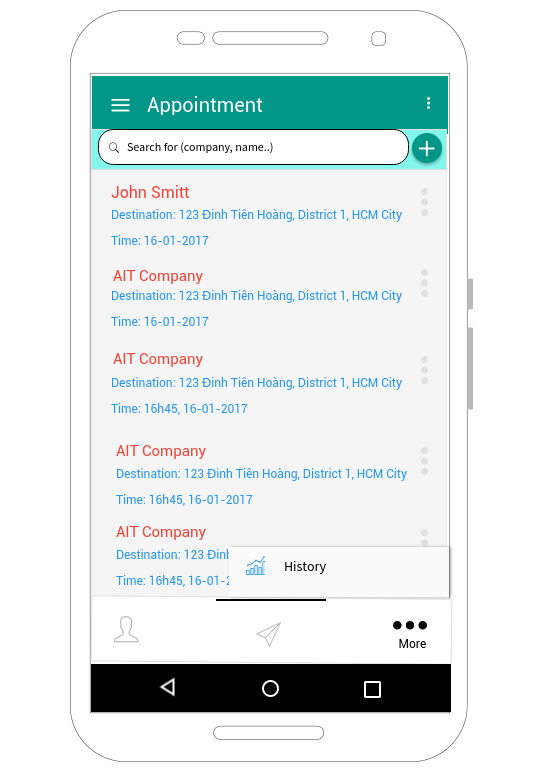
\includegraphics[scale=0.6]{Mockup/HI_redirecthistory}
    \centering
    \caption{Chuyển hướng chọn màn hình lịch sử}
    \label{fig:HI_redirecthistory}
\end{figure}
\begin{figure}[h]
    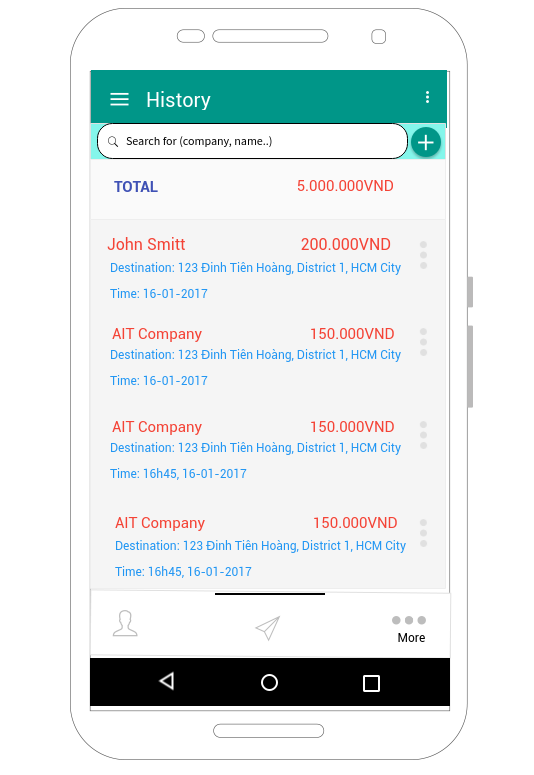
\includegraphics[scale=0.6]{Mockup/HI_history}
    \centering
    \caption{Màn hình lịch sử các điểm hẹn}
    \label{fig:HI_history}
\end{figure}
\begin{figure}[h]
    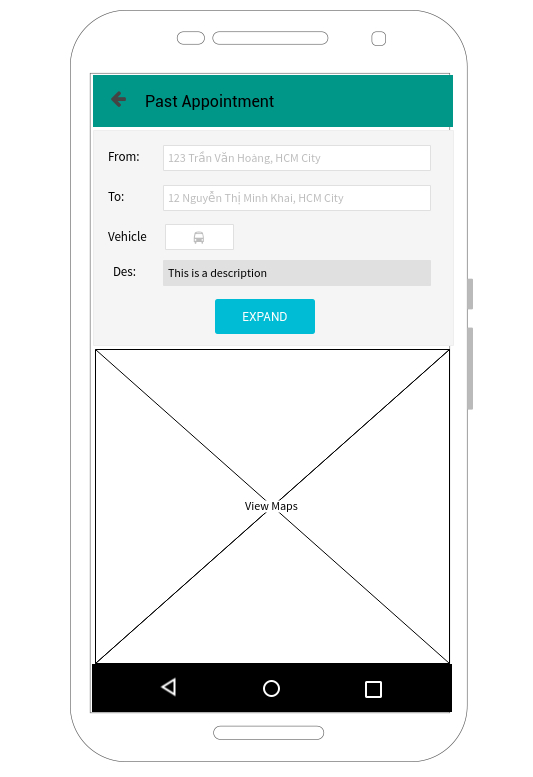
\includegraphics[scale=0.6]{Mockup/HI_pastappointment}
    \centering
    \caption{Màn hình chi tiết điểm hẹn trong lịch sử}
    \label{fig:HI_pastappointment}
\end{figure}
\clearpage
\subsection{Thiết kế Sequence Diagram}
Sau đây là các sequence diagram chính:
\begin{figure}[h]
    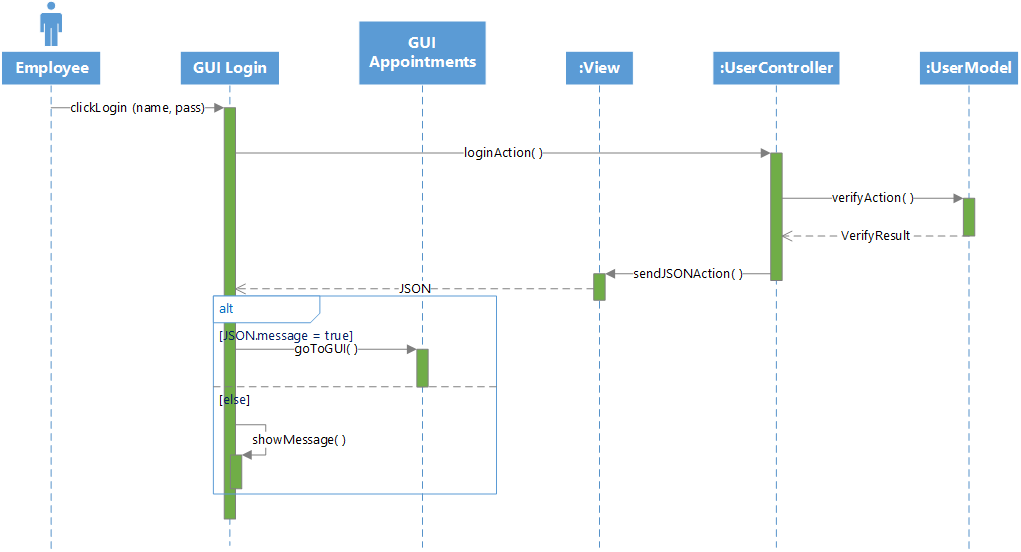
\includegraphics[width=13cm]{SequenceDiagram/Login}
    \centering
    \caption{Sequence diagram cho chức năng login}
    \label{fig:sequence_login}
\end{figure}
\begin{figure}[h]
    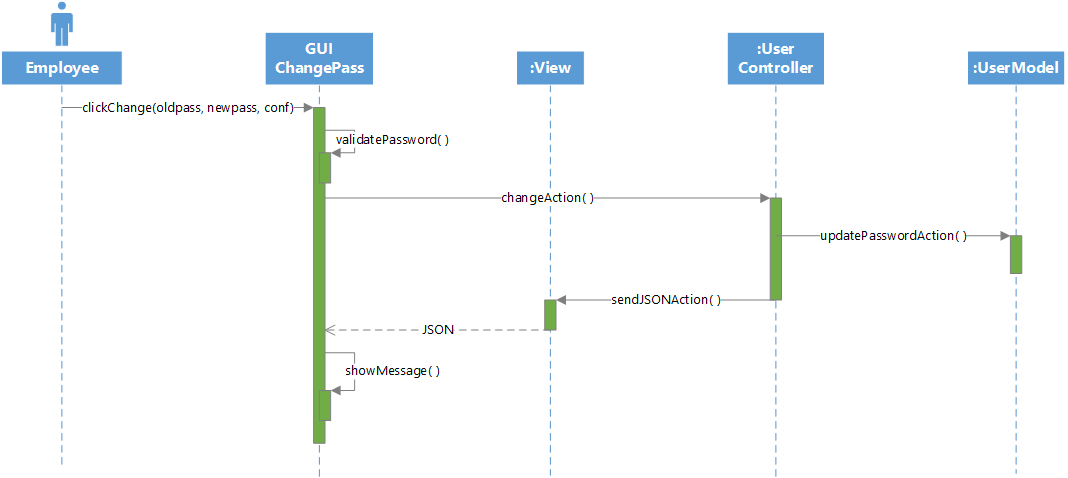
\includegraphics[width=13cm]{SequenceDiagram/ChangePassword}
    \centering
    \caption{Sequence diagram cho chức năng đổi mật khẩu}
    \label{fig:sequence_changepassword}
\end{figure}
\clearpage
\begin{figure}[!h]
    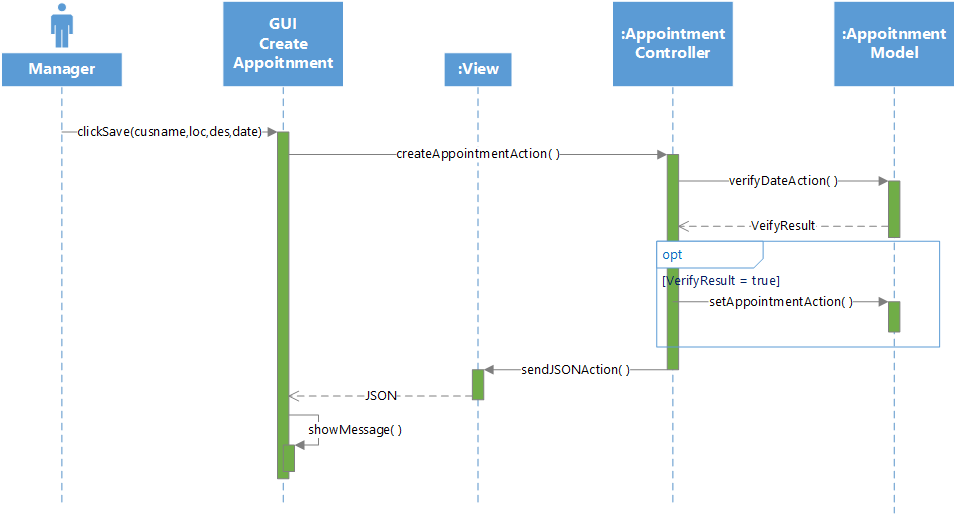
\includegraphics[width=13cm]{SequenceDiagram/CreateAppointment}
    \centering
    \caption{Sequence diagram cho chức năng tạo điểm hẹn}
    \label{fig:sequence_createappointment}
\end{figure}
\begin{figure}[!h]
    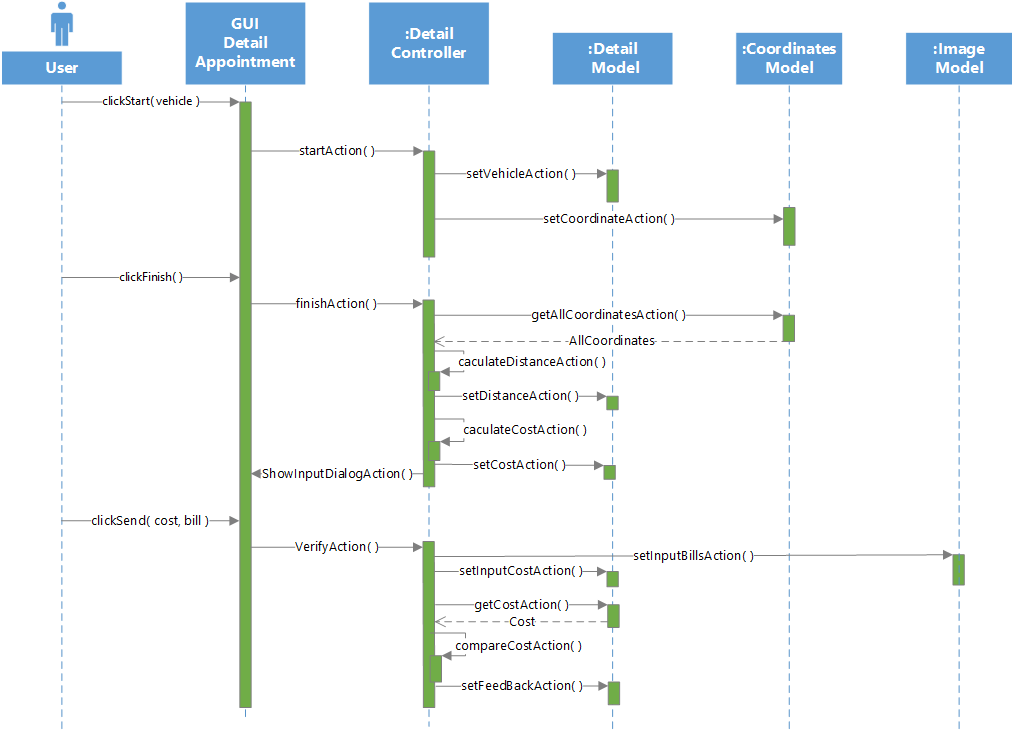
\includegraphics[width=13cm]{SequenceDiagram/Journey}
    \centering
    \caption{Sequence diagram cho chức năng đến một điểm hẹn}
    \label{fig:sequence_journey}
\end{figure}
\clearpage

\subsection{Thiết kế Activity Diagram}
\begin{figure}[!h]
    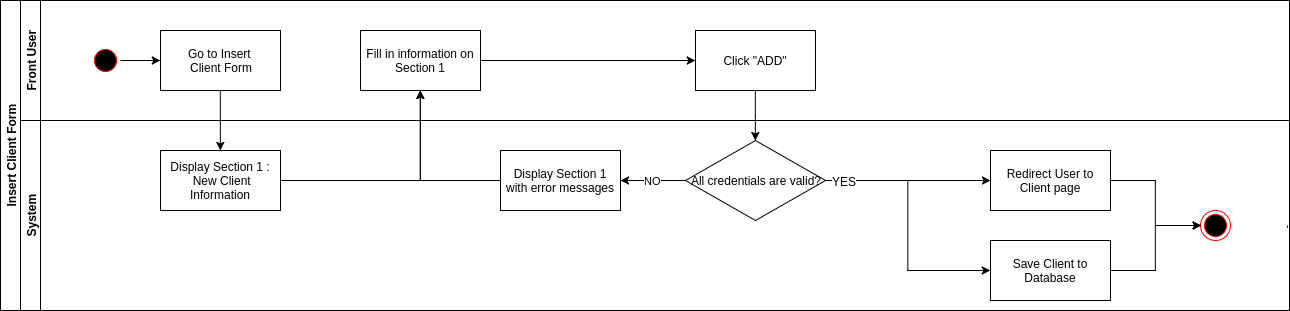
\includegraphics[width=14.7cm]{ActivityDiagram/AddCustomer}
    \centering
    \caption{Activity diagram cho chức năng thêm khách hàng}
    \label{fig:activity_add_customer}
\end{figure}
\begin{figure}[!h]
    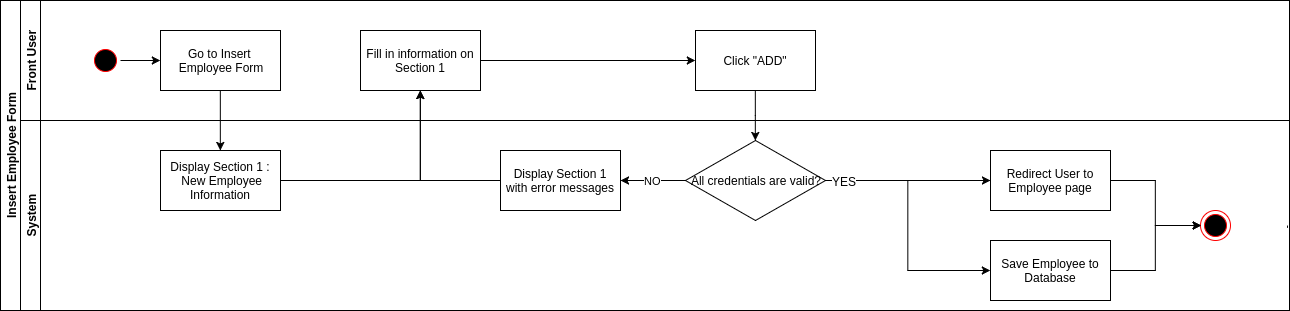
\includegraphics[width=14.7cm]{ActivityDiagram/AddEmployee}
    \centering
    \caption{Activity diagram cho chức năng thêm nhân viên}
    \label{fig:activity_add_employee}
\end{figure}
\begin{figure}[!h]
    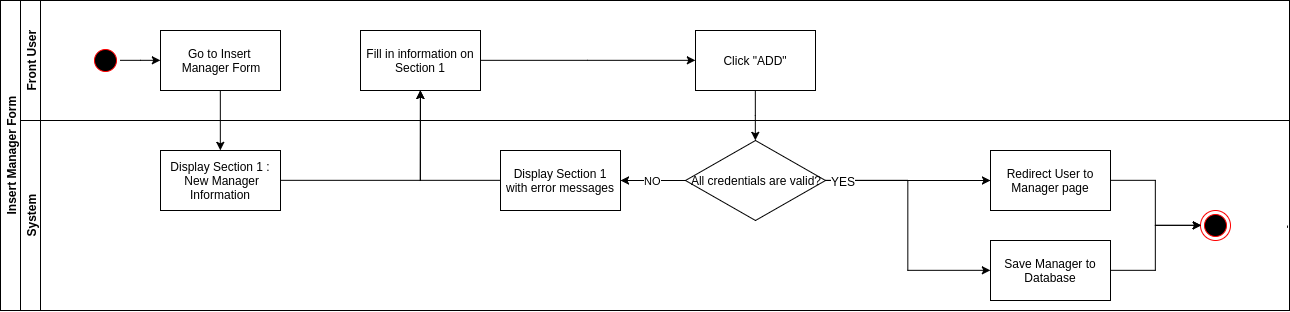
\includegraphics[width=14.7cm]{ActivityDiagram/AddManager}
    \centering
    \caption{Activity diagram cho chức năng thêm người quản lý}
    \label{fig:activity_add_manager}
\end{figure}
\clearpage
\begin{figure}[!h]
    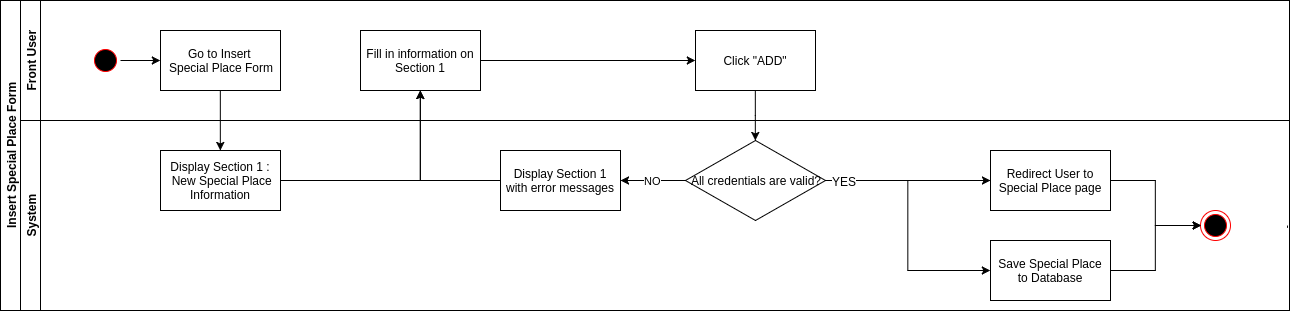
\includegraphics[width=14.7cm]{ActivityDiagram/AddSpecialPlace}
    \centering
    \caption{Activity diagram cho chức năng thêm vị trí đặc biệt}
    \label{fig:activity_add_special_place}
\end{figure}
\begin{figure}[!h]
    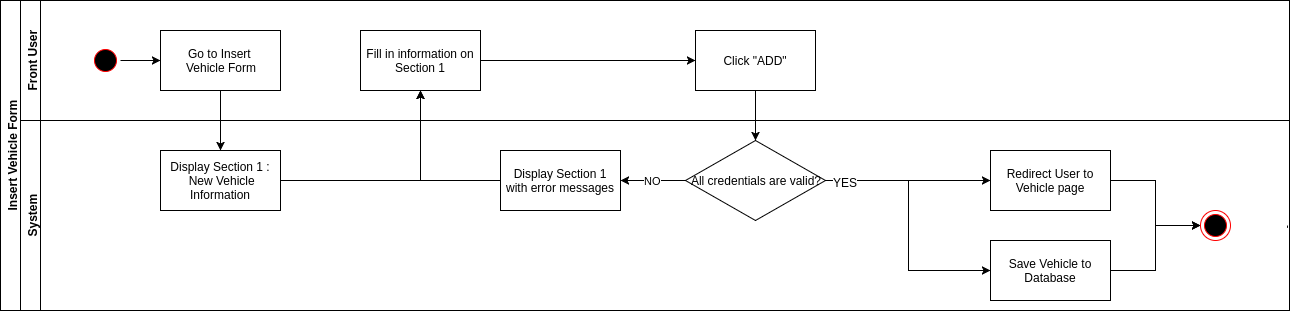
\includegraphics[width=14.7cm]{ActivityDiagram/AddVehicle}
    \centering
    \caption{Activity diagram cho chức năng thêm phương tiện}
    \label{fig:activity_add_vehicle}
\end{figure}
\begin{figure}[!h]
    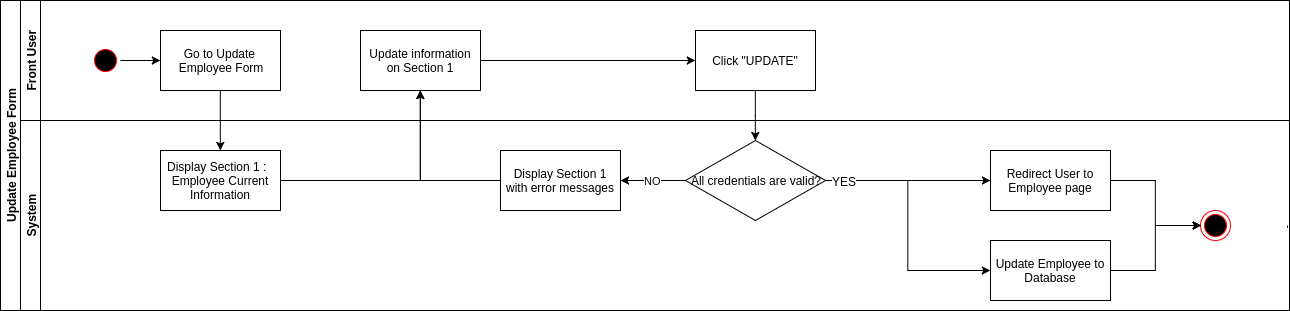
\includegraphics[width=14.7cm]{ActivityDiagram/EditEmployee}
    \centering
    \caption{Activity diagram cho chức năng chỉnh sửa nhân viên}
    \label{fig:activity_edit_employee}
\end{figure}
\begin{figure}[!h]
    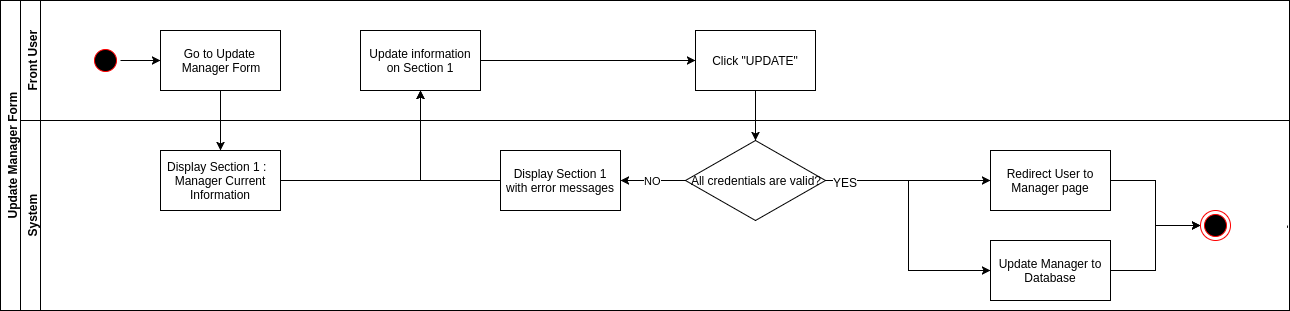
\includegraphics[width=14.7cm]{ActivityDiagram/EditManager}
    \centering
    \caption{Activity diagram cho chức năng chỉnh sửa người quản lý}
    \label{fig:activity_edit_manager}
\end{figure}
\begin{figure}[!h]
    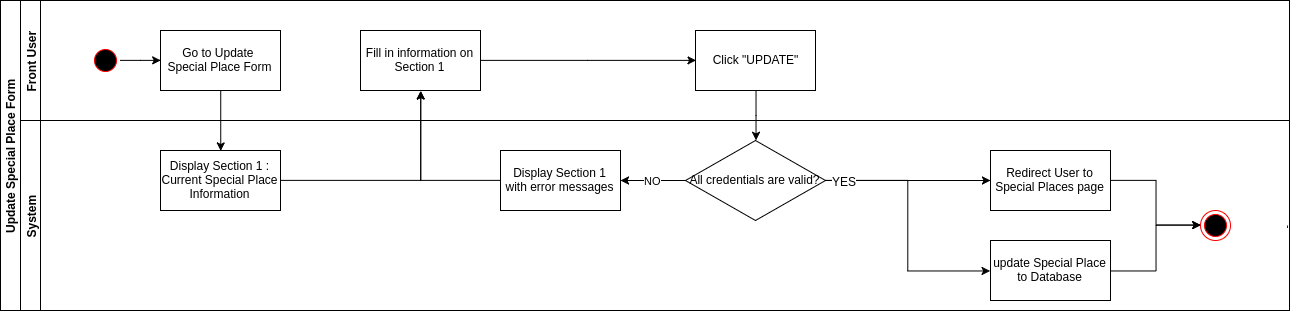
\includegraphics[width=14.7cm]{ActivityDiagram/EditSpecialPlace}
    \centering
    \caption{Activity diagram cho chức năng chỉnh sửa vị trí đặc biệt}
    \label{fig:activity_edit_special_place}
\end{figure}
%%%%%%%%%%%%%%%%%%%%%%%%%
%%%%%%%%%%%%%%%%%%%%%%%%%
\subsection{Danh sách các hàm được sử dụng}
\begin{longtable}{ | p{.15\textwidth} |p{.30\textwidth} | p{.50\textwidth}  | } 
\hline
\textbf{Tên hàm}& \textbf{Chức năng}& \textbf{Thông số đầu vào} \\ 
\hline

\hline
Create Appointment & 
Tạo một công tác và lưu vào trong cơ sở dữ liệu. &
Một JSON Object bao gôm các trường:
\begin{itemize}
  \item “destination” : đích đến của công tác(Chuỗi).
  \item “startdate” : ngày bắt đầu dự kiến của công tác(Chuỗi  có dạng HH:mm dd-MM-yyyy).
  \item “users” : danh sách mã số những người tham gia công tác(Chuỗi có dạng 1,2,3,4).
  \item “clientid” : mã số của khách hàng đã được lưu trong cơ sở dữ liệu(Số  nguyên). 
\end{itemize}
  \\ 
\hline
Get Active Appointments & 
Lấy danh sách các công tác chưa kết thúc trong cơ sở dữ liệu. &
không có tham số nào. \\

\hline
Get Completed Appointments & 
Lấy danh sách các công tác đã kết thúc trong cơ sở dữ liệu. &
không có tham số nào. \\ 

\hline
Update Appointment & 
Cập nhật thông tin một công tác đã tồn tại trong cơ sở dữ liệu (chỉ dùng cho người quản lý). &
Một JSON Object bao gôm các trường: 
\begin{itemize}
  \item “\verb|destination|” : đích đến của công tác (Chuỗi). 
  \item “\verb|start_date|” : ngày bắt đầu dự kiến của công tác (Chuỗi  có dạng HH:mm dd-MM-yyyy).
  \item “\verb|users|” : danh sách mã số những người tham gia công tác(Chuỗi có dạng 1,2,3,4).
  \item “\verb|client_id|” : mã số của khách hàng đã được lưu trong cơ sở dữ liệu(Số  nguyên).
  \item “\verb|appointment_id|” : mã số của công tác ta muốn cập nhật (Số nguyên). 
\end{itemize}
\\ 

\hline
End Appointment  & 
Kết thúc một công tác và cập nhật vào cơ sở dữ liệu. &
Một JSON Object bao gôm các trường: 
\begin{itemize}
  \item “\verb|id|” : mã số của công tác (Số nguyên).  
  \item “\verb|end_date|” : thời gian kết thúc của công tác (Chuỗi có dạng HH:mm dd-MM-yyyy).
\end{itemize}
\\ 

\hline
Create Client & 
Tạo một khách hàng và lưu vào trong cơ sở dữ liệu. &
Một JSON Object bao gôm các trường: 
\begin{itemize}
  \item “\verb|name|” : tên của khách hàng (Chuỗi).  
  \item “\verb|phone_number|” :số điện thoại của khách hàng (Chuỗi số bao gôm 10-11 số nhất và chỉ được thêm khoảng trắng). 
  \item “\verb|address|” :  địa chỉ của khách hàng (Chuỗi).
  \item “\verb|email|” : email của khách hàng (Chuỗi tuân theo đúng định dạng email).
\end{itemize}
\\ 

\hline
Get Clients & 
Lấy danh sách các khách hàng đã lưu trong cơ sở dữ liệu. &
không có thông số nào.
\\ 

\hline
Get Client Info & 
Lấy thông tin chi tiết của một khách hàng . &
Một JSON Object chứa một trường duy nhất là mã số của khách hàng (Số nguyên).
\\ 

\hline
Add Coordinate & 
Thêm một (hoặc nhiều) tọa độ vị trí cho một lịch trình. &
Một JSON Object bao gôm các trường: 
\begin{itemize}
  \item “\verb|detail_id|” : mã số của lịch trình.  
\item “\verb|coordinates|” :mảng các tọa độ (JSON Array) có cấu trúc của một phần tử bao gồm ba trường : “latitude” (vĩ độ - Số thực), “longitude”(kinh độ - số thực) và
“time”(thời gian - chuỗi có dạng HH:mm:ss dd-MM-yyyy).
\end{itemize}
\\ 

\hline
Create Detail & 
Tạo một lịch trình và lưu vào trong cơ sở dữ liệu, đồng thời ta cũng bắt đầu luôn lịch trình này. &
Một JSON Object bao gôm các trường: 
\begin{itemize}
  \item “\verb|vehicle_id|” : : mã số của phương tiện (Số nguyên).  
  \item “\verb|start_time|” : thời gian bắt đầu của lịch trình (Chuỗi  có dạng HH:mm:ss dd-MM-yyyy).
  \item “\verb|start_location|”: thời gian bắt đầu của lịch trình (Chuỗi  có dạng HH:mm:ss dd-MM-yyyy).
  \item “\verb|appointment_id|”: mã số của công tác đã được lưu trong cơ sở dữ liệu (Số  nguyên). 
\end{itemize}
\\ 


\hline
End Detail  & 
Kết thúc một lịch trình. &
Một JSON Object bao gôm các trường: 
\begin{itemize}
  \item “\verb|image_content|” : hình ảnh hóa đơn được người dùng chụp lại, đây là một chuỗi có nội dung là base 64 của file hình ảnh, có thể rỗng. 
  \item “\verb|description|” : ghi chú của lịch trình này (kẹt xe, bể bánh, thêm tiền...) (Chuỗi).
  \item “\verb|input_cost|”: số tiền phải trả để thực hiện lịch trình (Số thực).
\end{itemize}
\\ 

\hline
Get Employees & 
Lấy danh sách các nhân viên dưới quyền quản lý (chỉ dùng cho người quản lý).&
Một JSON Object bao một trường duy nhất là mã số của người dùng (Số nguyên).
\\ 

\hline
Get User Info  & 
Lấy thông tin chi tiết của một người dùng. &
Một JSON Object bao một trường duy nhất là mã số của người dùng (Số nguyên).
\\

\hline
Get Vehicles   & 
Lấy danh sách các phương tiện đi lại. &
không có tham số nào.
\\
 
\hline

\caption{Bảng các hàm chính được sử dụng của hệ thống}
\end{longtable}
\section{Hiện thực dự án}
\subsection{Công nghệ sử dụng}
Để hiện thực đề tài này, chúng tôi sử dụng một số công nghệ và ứng dụng sau : 
\begin{longtable}{ | p{.20\textwidth} |p{.30\textwidth} | p{.50\textwidth}  | } 
\hline
\textbf{Công nghệ và ứng dụng}& \textbf{Phiên bản}& \textbf{Ghi chú} \\ 
\hline
\hline
Spring Framework &
4.0.6 &
Công nghệ chủ đạo của phía Server.
\\ 
\hline
Android  &
5.0 trở lên &
Công nghệ chủ đạo của phía Client.
\\ 
\hline
Java  &
8.0 &
Công nghệ chủ đạo của phía Client.
\\ 
\hline
Apache  &
2.2.11 &
Công nghệ chủ đạo của phía Client.
\\ 
\hline
PostgreSQL  &
10 &
Cơ sở dữ liệu của toàn bộ hệ thống.
\\ 

\hline

\caption{Bảng các công nghệ sử dụng}
\end{longtable}
\subsection{Client}
\subsubsection{Tổ chức dự án}
Cấu trúc mã nguồn ban đầu được viết dựa trên cấu trúc mặc định được Android Studio cung cấp (được thể hiện ở hình \ref{fig:client_architecture})\\
\begin{figure}[!h]
    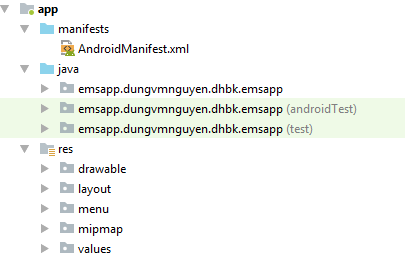
\includegraphics[scale=1]{Client/client-architecture}
    \centering
    \caption{Cấu trúc mã nguồn mặc định của Android Studio}
    \label{fig:client_architecture}
\end{figure}
\par
Cấu trúc cây thư mục gồm 3 phần chính:
\begin{itemize}
  \item \texttt{Thư mục manifests:} chứa các cài đặt cần thiết cho ứng dụng. 
  \item \texttt{Thư mục java:} chứa mã nguồn xử lý back-end cho ứng dụng.
  \item \texttt{Thư mục res:} chứa mã nguồn dùng cho giao diện của ứng dụng.
\end{itemize}
\begin{figure}[!h]
    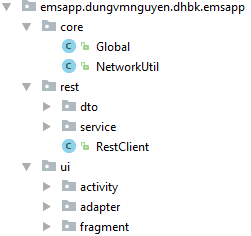
\includegraphics[scale=1]{Client/project-architecture}
    \centering
    \caption{Cấu trúc mã nguồn mặc định của Android Studio}
    \label{fig:project_architecture}
\end{figure}
Cấu trúc của thư mục \textbf{java/emsapp/dungvmnguyen/dhbk/emsapp} bao gồm 3 package chính: \texttt{core, rest, ui.} Trong đó:
\begin{itemize}
\item \texttt{Pakage core:} chứa mã nguồn dùng cho việc xử lý kết nối mạng của thiết bị và lưu trữ lại các biến toàn cục.
\item \texttt{Package res:} chứa mã nguồn hiện thực các \texttt{service} và các \texttt{dto}.
\item \texttt{Package ui:} chứa các \texttt{activity, adapter, fragment} của ứng dụng.
\end{itemize}
Cấu trúc của thư mục res bao gồm 3 thư mục chính: \texttt{drawable, layout, menu, mipmap, values.} Trong đó:
\begin{itemize}
\item \texttt{Thư mục drawable:} chứa các hình ảnh được sử dụng trong ứng dụng
\item \texttt{Thư mục layout:} chứa tập hợp các file .xml dùng để hiện thực giao diện của ứng dụng
\item \texttt{Thư mục menu:} chứa file \texttt{activity\_main\_drawer.xml} hiện thực giao diện của thanh danh sách các chức năng bên trái màn hình ứng dụng.
\item \texttt{Thư mục mipmap:} chứa các icon mặc định của ứng dụng.
\item \texttt{Thư mục values:} tập hợp các file .xml chứa các khai báo cần thiết cho ứng dụng.
\end{itemize}
\clearpage
\subsubsection{Kết quả đạt được}
\textbf{Màn hình đăng nhập}\\\\
Khi khởi động ứng dụng, hệ thống yêu cầu người dùng đăng nhập vào hệ thống.\\\\
Hệ thống sẽ xác thực và phân loại người dùng để cung cấp những chức năng phù hợp.\\  
\begin{figure}[!h]
  \fbox{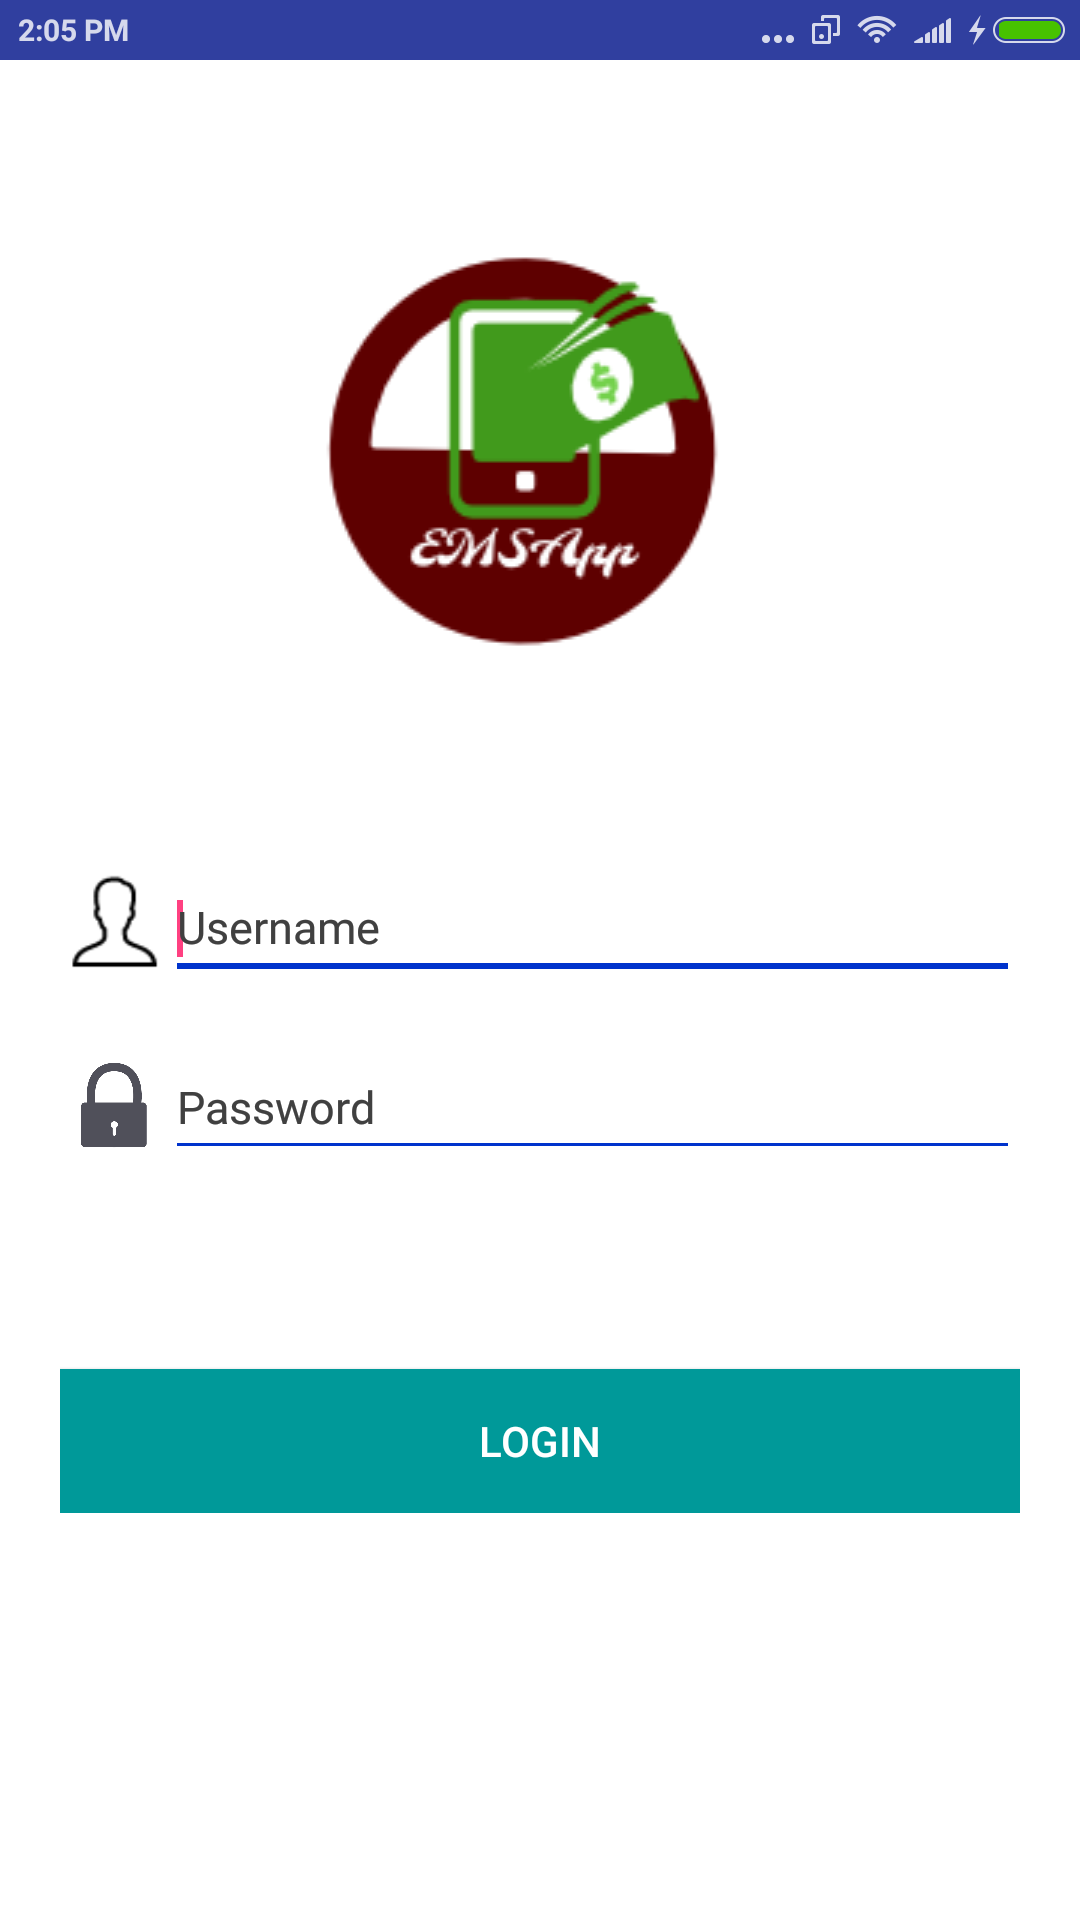
\includegraphics[scale=0.13]{/Client/UI/login}} 
    \centering
    \caption{Trang đăng nhập}
    \label{fig:ui_login}
\end{figure} 
\\
\textbf{Màn hình chính}\\\\
Sau khi đăng nhập thành công, nếu người dùng là nhân viên thì sẽ được hệ thống chuyển tới màn hình danh sách các cuộc hẹn.\\\\
Tại đây người dùng sẽ thấy các thông tin cơ bản của một cuộc hẹn bao gồm \textit{tên cuộc hẹn, địa điểm, thời gian diễn ra cuộc hẹn.}\\\\
Để bắt đầu một cuộc hẹn, người dùng nhấn chọn một cuộc hẹn trong danh sách.\\
\begin{figure}[!h]
  \fbox{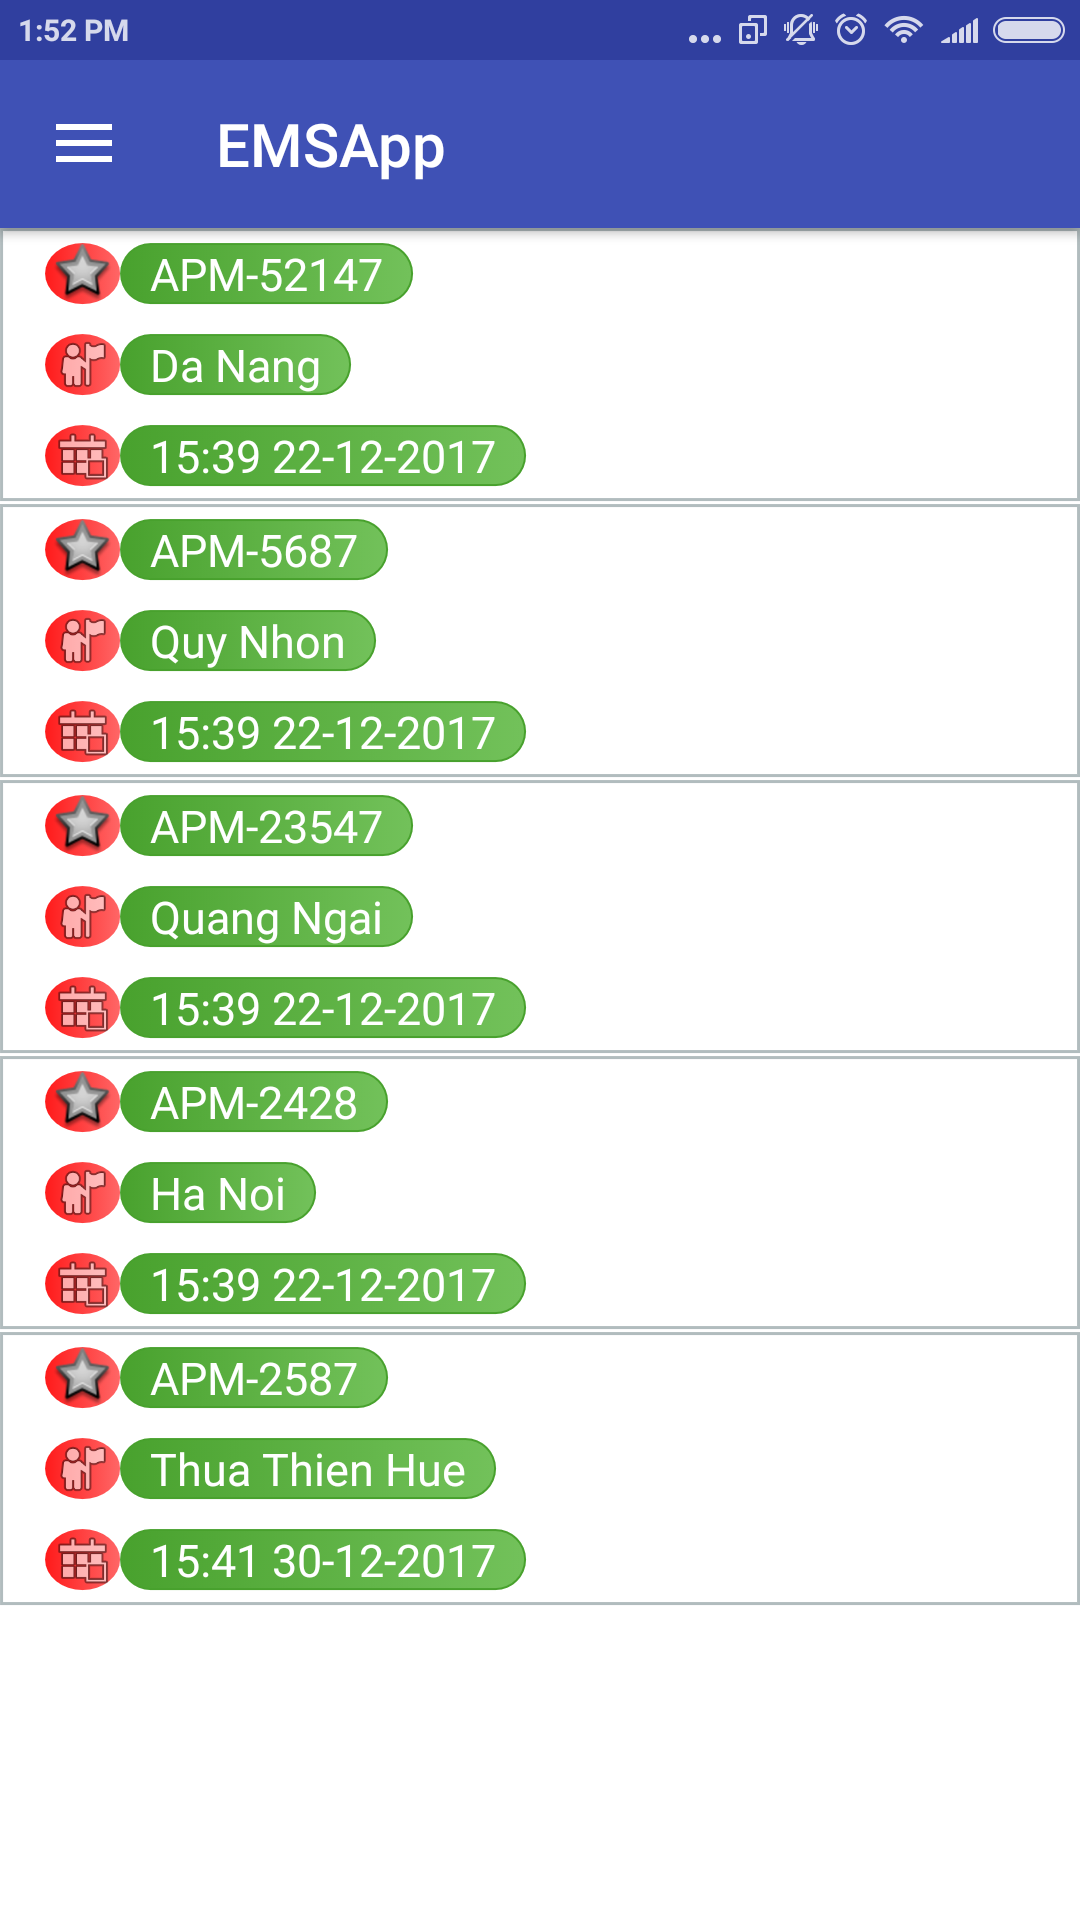
\includegraphics[scale=0.11]{/Client/UI/home}} 
    \centering
    \caption{Màn hình chính khi User đăng nhập là Employee}
    \label{fig:ui_home}
\end{figure} 
\\
Nếu người dùng là người quản lý, người dùng sẽ được chuyển tới trang danh sách các nhân viên do mình quản lý.\\\\
Tại đây người quản lý có thể thông tin cơ bản của các nhân viên bao gồm \textit{họ tên, email, loại nhân viên.}\\\\
Người quản lý nhấn chọn vào một nhân viên trong danh sách để xem thông tin chi tiết.\\
\begin{figure}[!h]
  \fbox{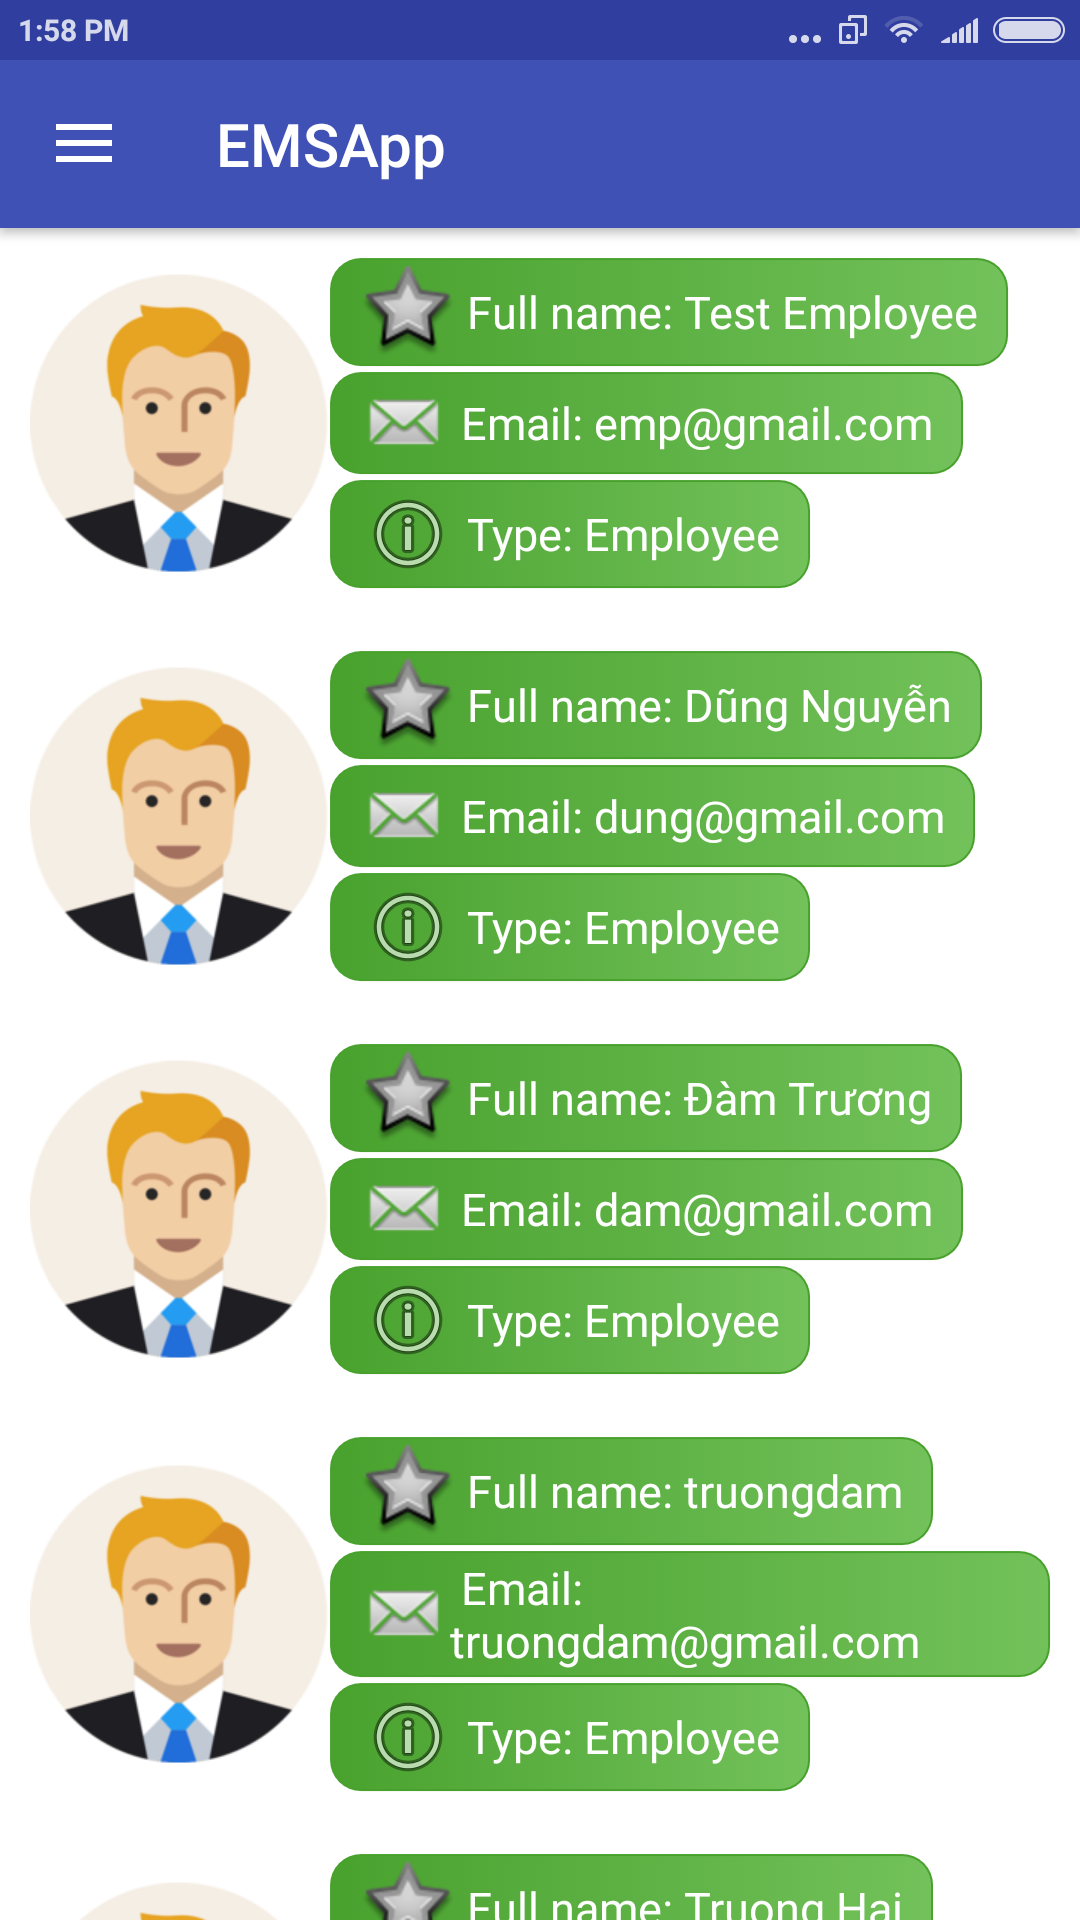
\includegraphics[scale=0.11]{/Client/UI/employee-list}} 
    \centering
    \caption{Màn hình chính khi User đăng nhập là Manager}
    \label{fig:ui_employee_list}
\end{figure} 
\\
Ở góc trái trên của màn hình chính, người dùng có thể nhấn chọn biểu tượng $\equiv$ hiển thị danh sách các chức năng của ứng dụng.\\\\
Tùy thuộc vào vai trò của người dùng mà hệ thống sẽ cho phép sử dụng một số chức năng nhất định.\\
\begin{figure}[!h]
  \fbox{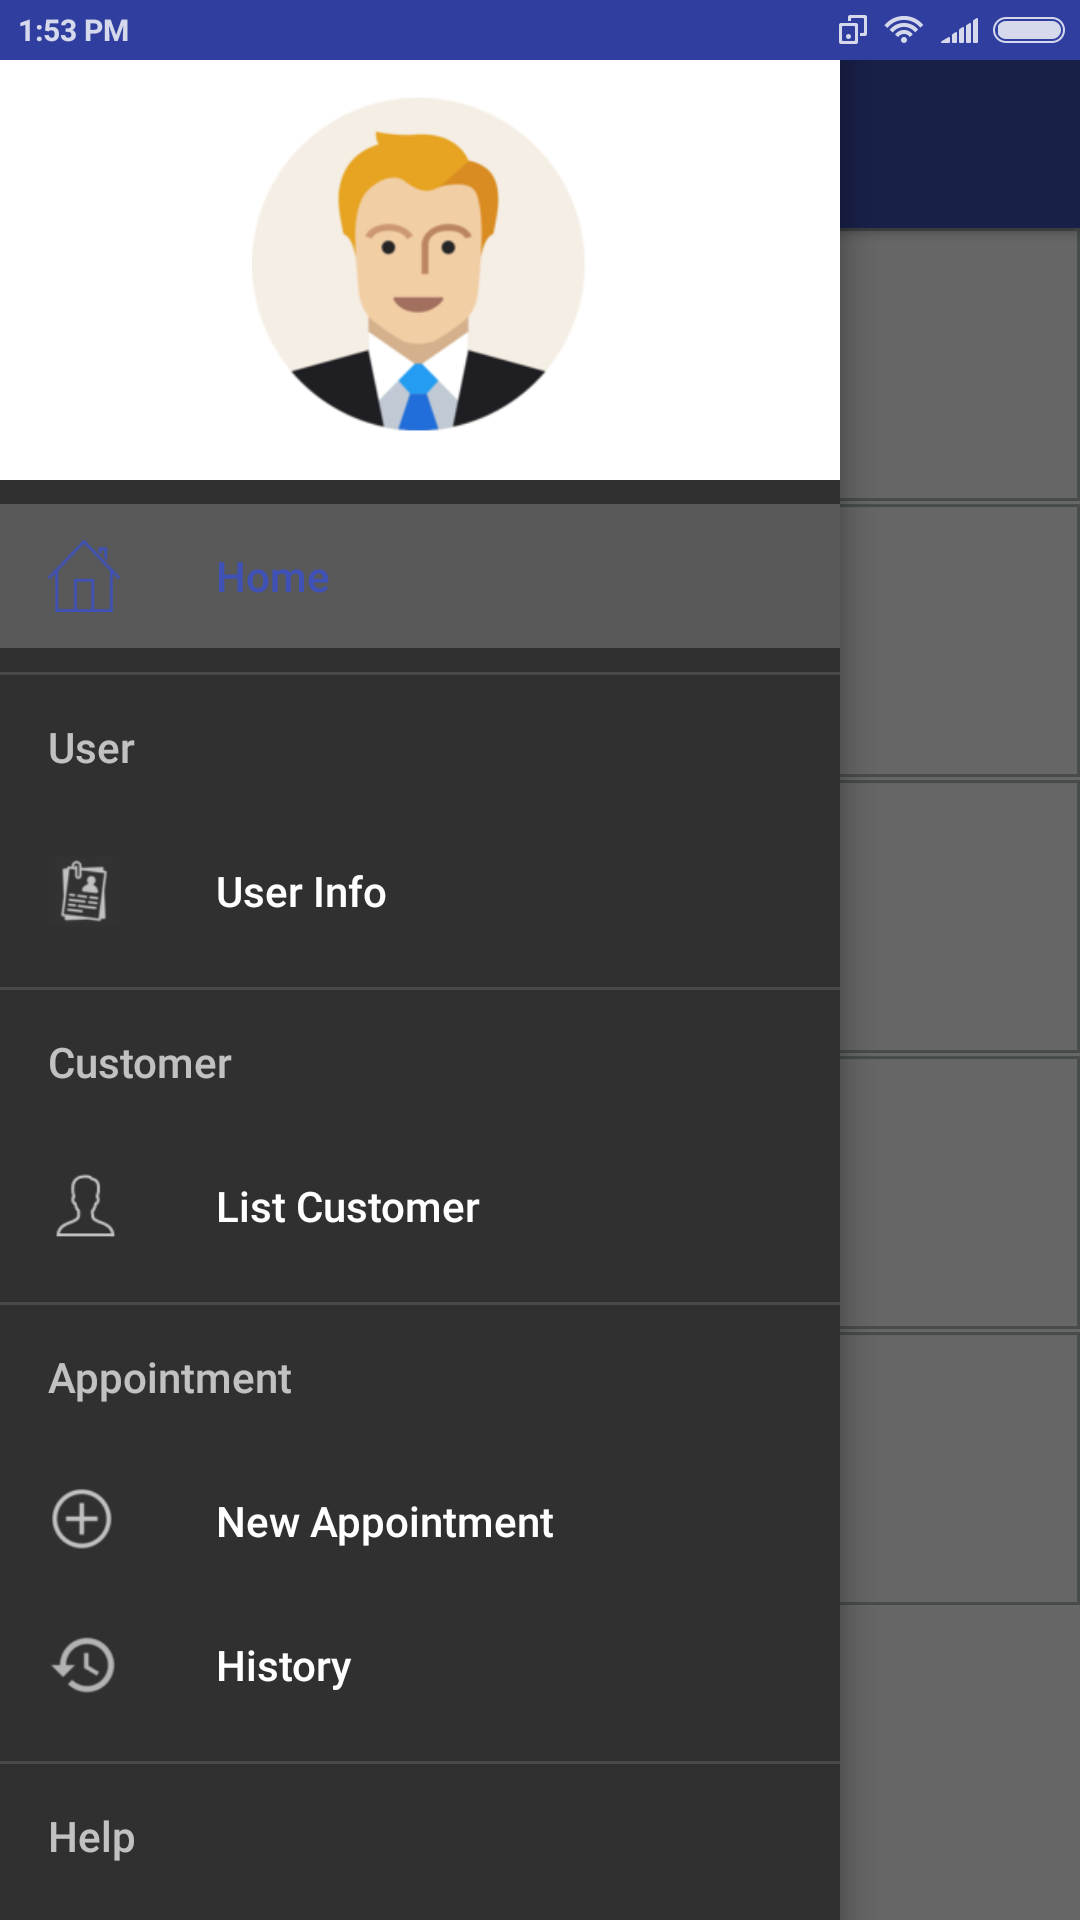
\includegraphics[scale=0.1]{/Client/UI/gadget}} 
    \centering
    \caption{Menu danh sách các chức năng}
    \label{fig:ui_employee_list}
\end{figure} 
\\
\textbf{Màn hình bắt đầu một lịch trình}\\\\
Sau khi người dùng chọn một cuộc hẹn trong danh sách, hệ thống sẽ hiển thị lên màn hình tiến hành một cuộc hẹn.\\
\begin{figure}[!h]
  \fbox{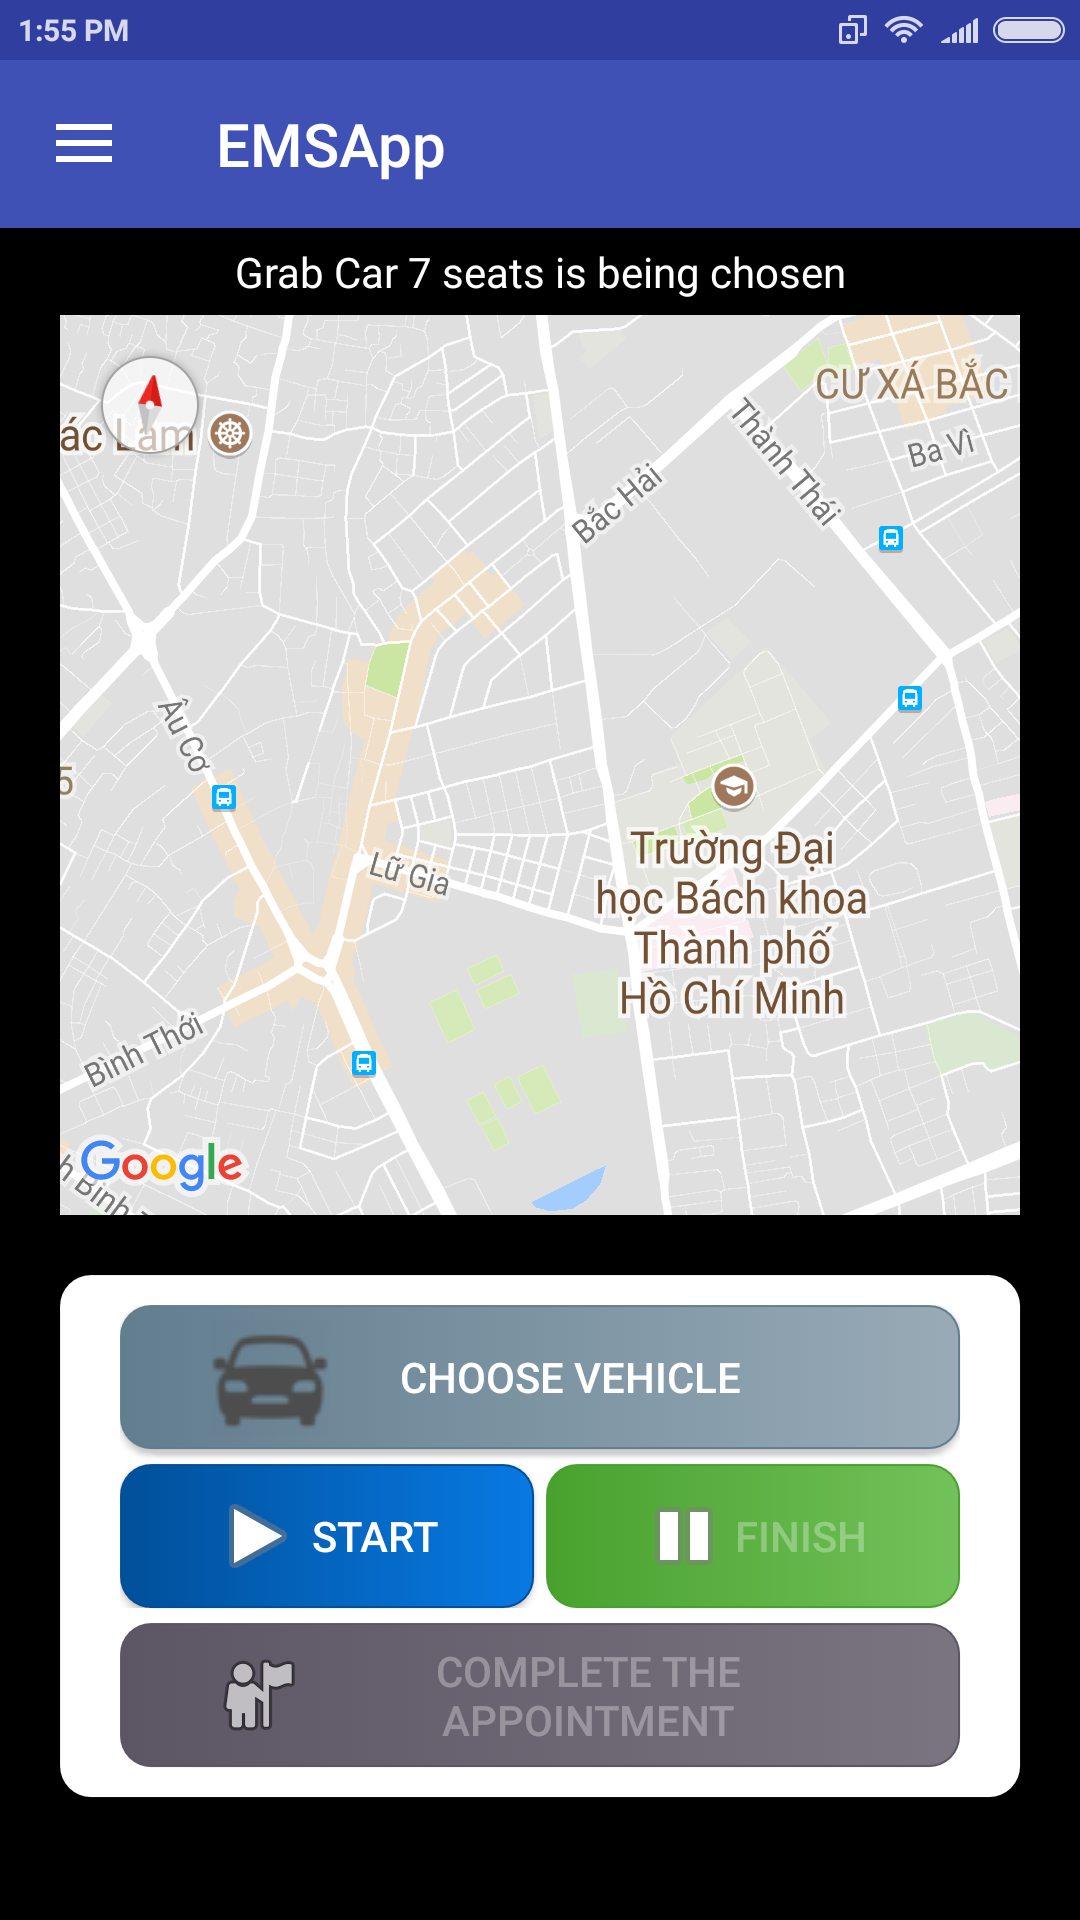
\includegraphics[scale=0.1]{/Client/UI/start-appointment}} 
    \centering
    \caption{Màn hình bắt đầu một cuộc hẹn}
    \label{fig:ui_employee_list}
\end{figure} 
\\
Đầu tiên người dùng sẽ lựa chọn phương tiện mình sử dụng để di chuyển.\\\\
Tại đây người dùng có thể xem một số thông tin cơ bản của phương tiện bao gồm tên phương tiện, mã phương tiện.\\
\begin{figure}[!h]
  \fbox{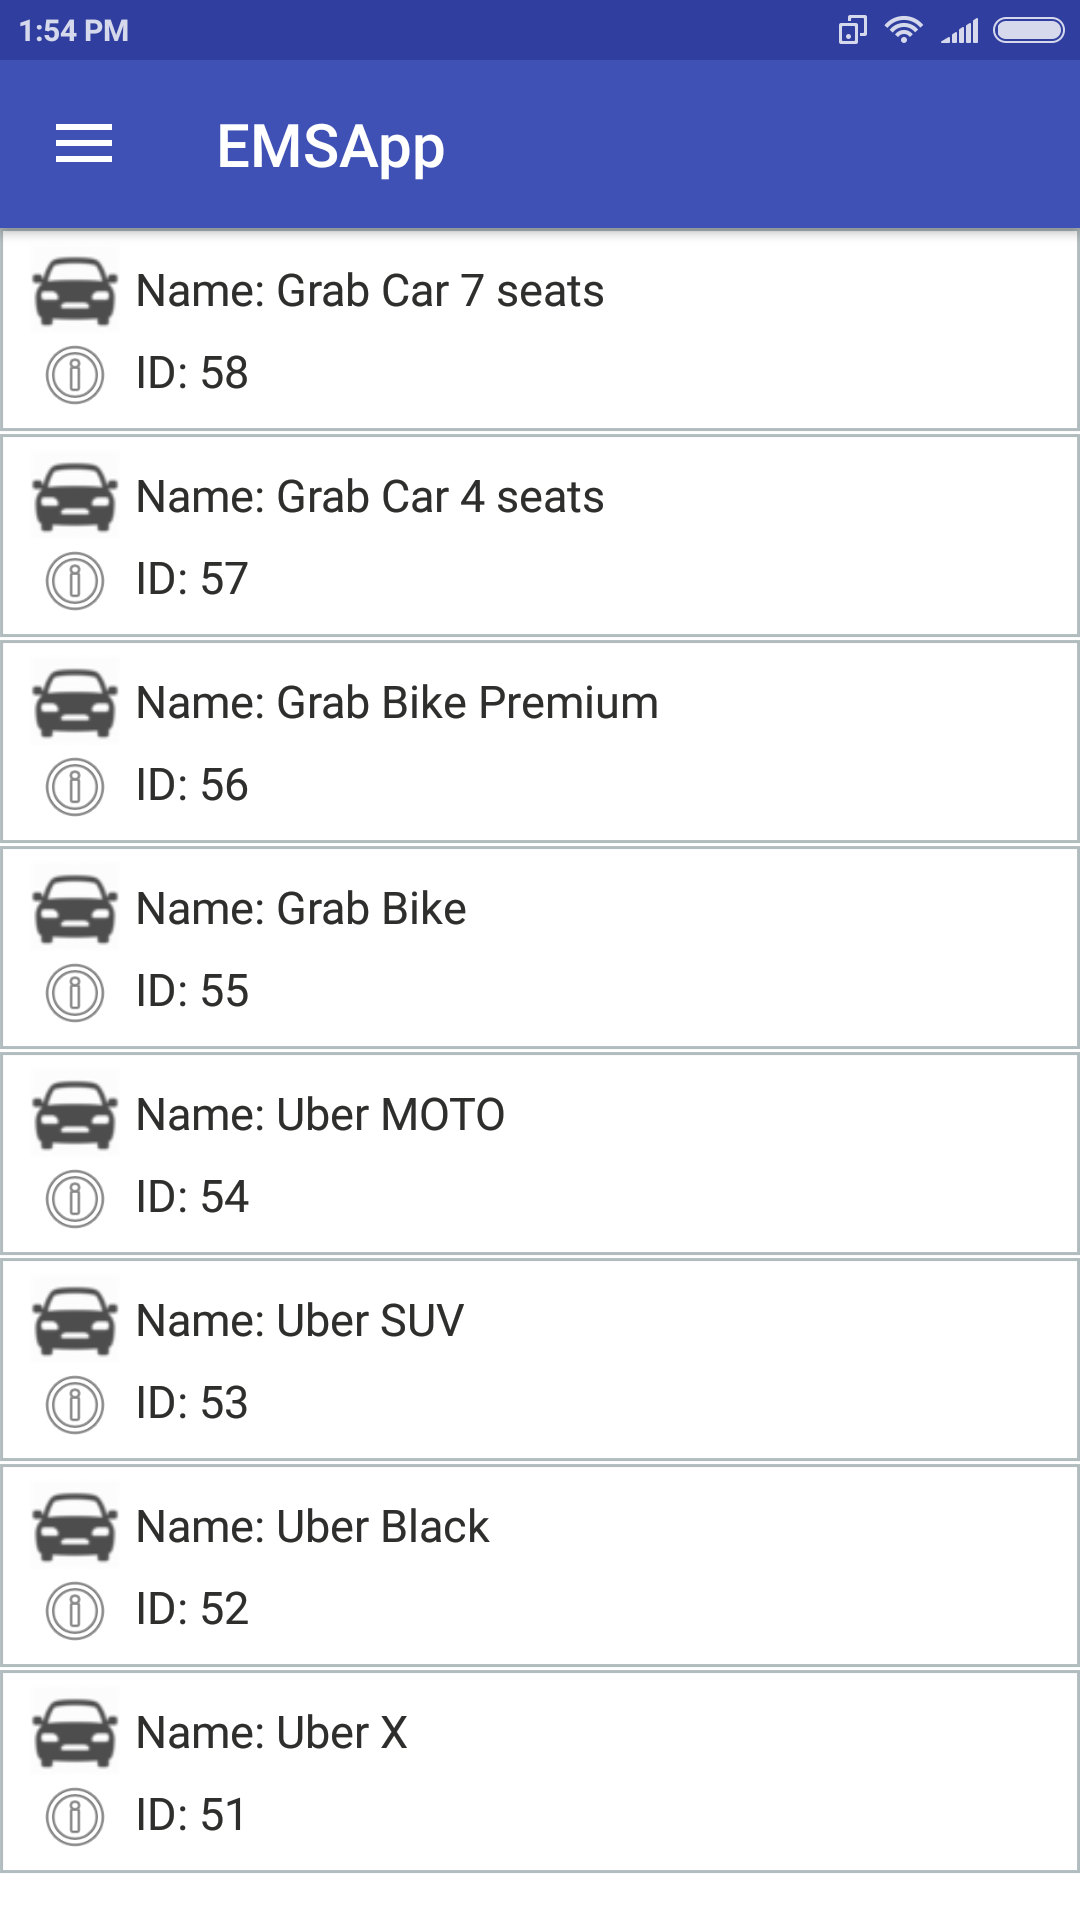
\includegraphics[scale=0.13]{/Client/UI/vehicle-list}} 
    \centering
    \caption{Màn hình chọn phương tiện di chuyển}
    \label{fig:ui_employee_list}
\end{figure} 
\\
Sau khi chọn phương tiện di chuyển, ứng dụng sẽ quay lại màn hình bắt đầu cuộc hẹn.\\\\
Khi bắt đầu di chuyển người dùng bấm chọn nút START để hệ thống bắt đầu tính toán. Trong quá trình di chuyển, hệ thống sẽ lưu tại tọa độ, thời gian để sử dụng cho việc tính toán chi phí sau khi kết thúc di chuyển đối với một phương tiện. Đồng thời hệ thống cũng vẽ ra quãng đường di chuyển trong suốt hành trình để cho người dùng có thể quan sát quãng đường đi lại của mình.\\\\
Người dùng nhấn chọn nút FINISH để kết thúc việc di chuyển bằng phương tiện hiện tại.Sau đó hệ thống sẽ bắt buộc người dùng nhập chi phí đi lại đối với phương tiện hiện tại. Đồng thời hệ thống cũng hỗ trợ chức năng chụp và gửi hóa đơn về cho hệ thống.\\
\begin{figure}[!h]
  \fbox{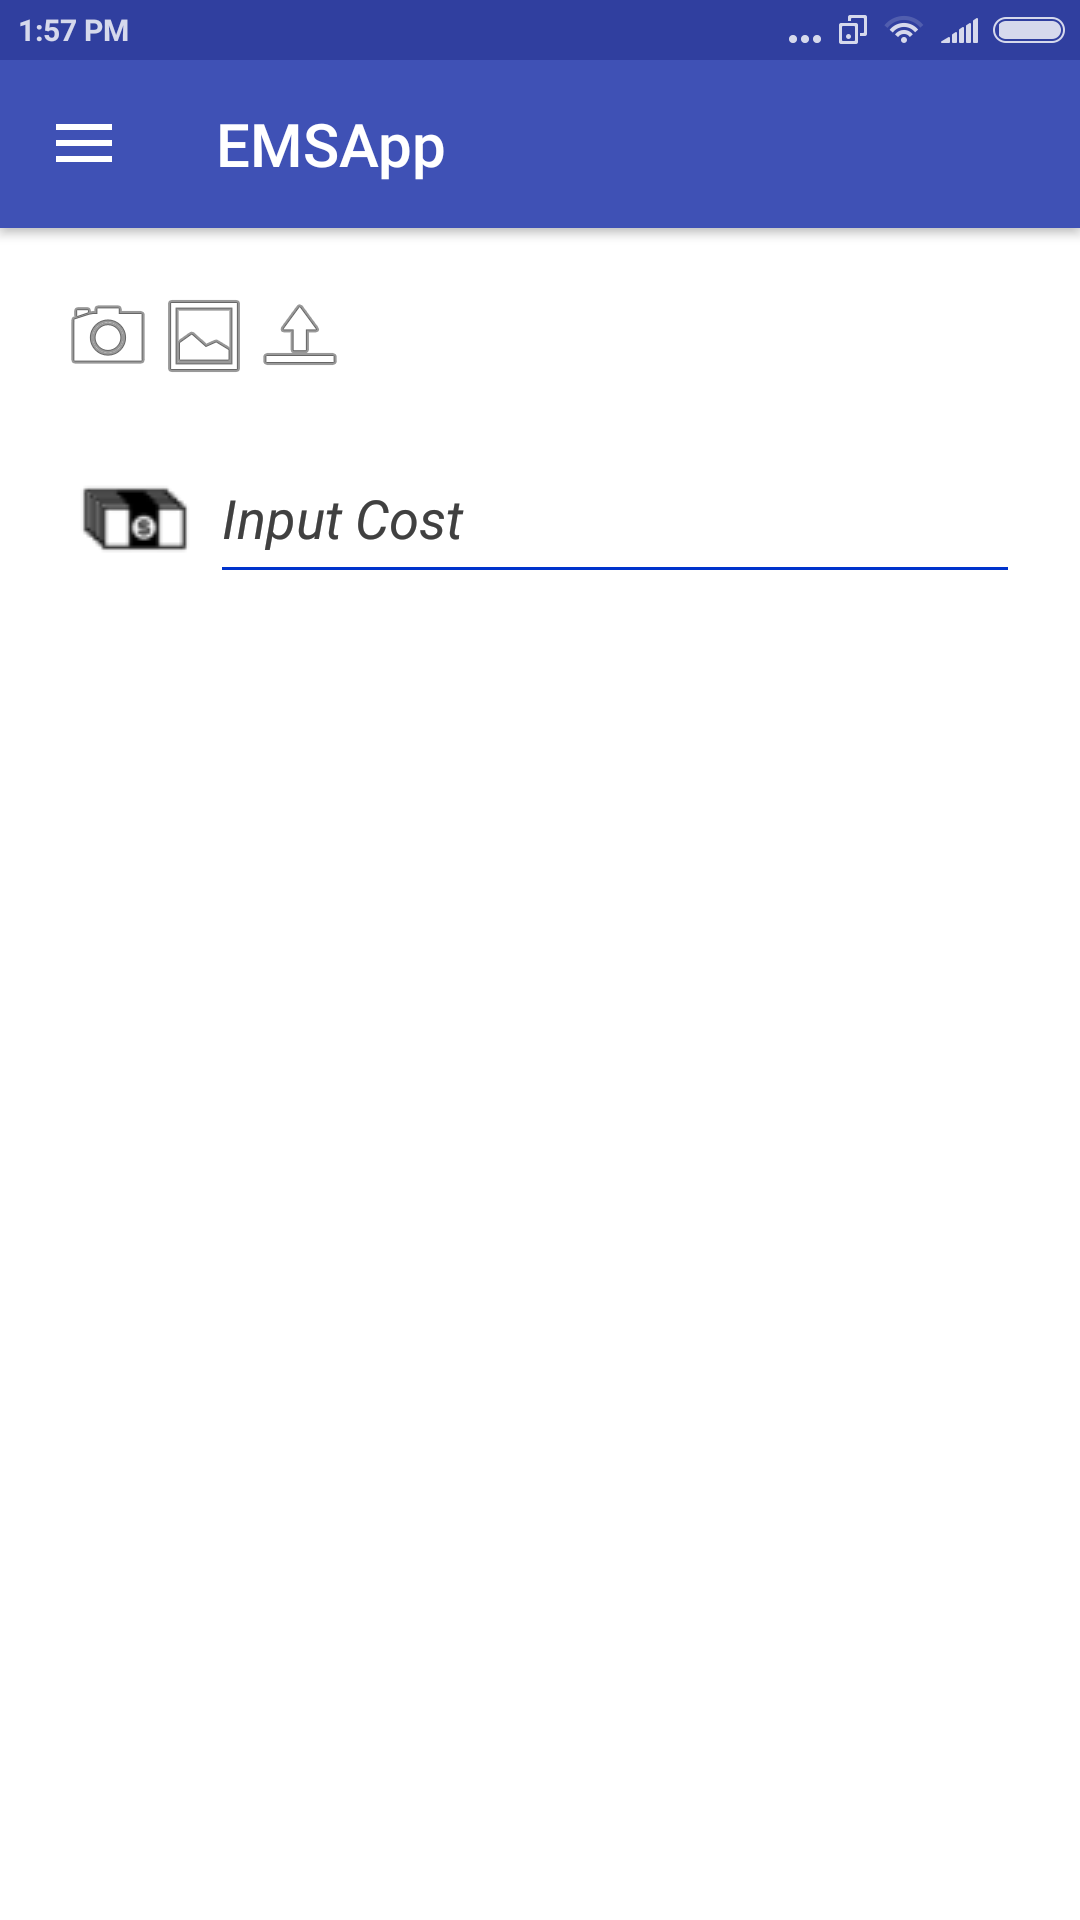
\includegraphics[scale=0.13]{/Client/UI/input-cost}} 
    \centering
    \caption{Màn hình nhập chi phí và hóa đơn}
    \label{fig:ui_employee_list}
\end{figure} 
\\
Lúc này người dùng có thể lựa chọn kết thúc cuộc hẹn hiện hoặc tiếp tục di chuyển bằng phương tiện khác. Để di chuyển bằng phương tiện khác người dùng đơn giản chỉ cần thực hiện lại các bước như ban đầu. Ngược lại để kết thúc cuộc hẹn, người dùng chọn nút COMPLETE THE APPOINTMENT.\\\\
\clearpage
\noindent
\textbf{Màn hình xem lịch sử các lịch trình đã hoàn thành}\\\\
Người dùng có thể chọn chức năng History để xem lại thông tin của các cuộc hẹn đã hoàn thành.\\\\
Người dùng có thể xem được một số thông tin cơ bản như tên cuộc hẹn, địa điểm, thời gian diễn ra, chi phí đi lại.\\
\begin{figure}[!h]
  \fbox{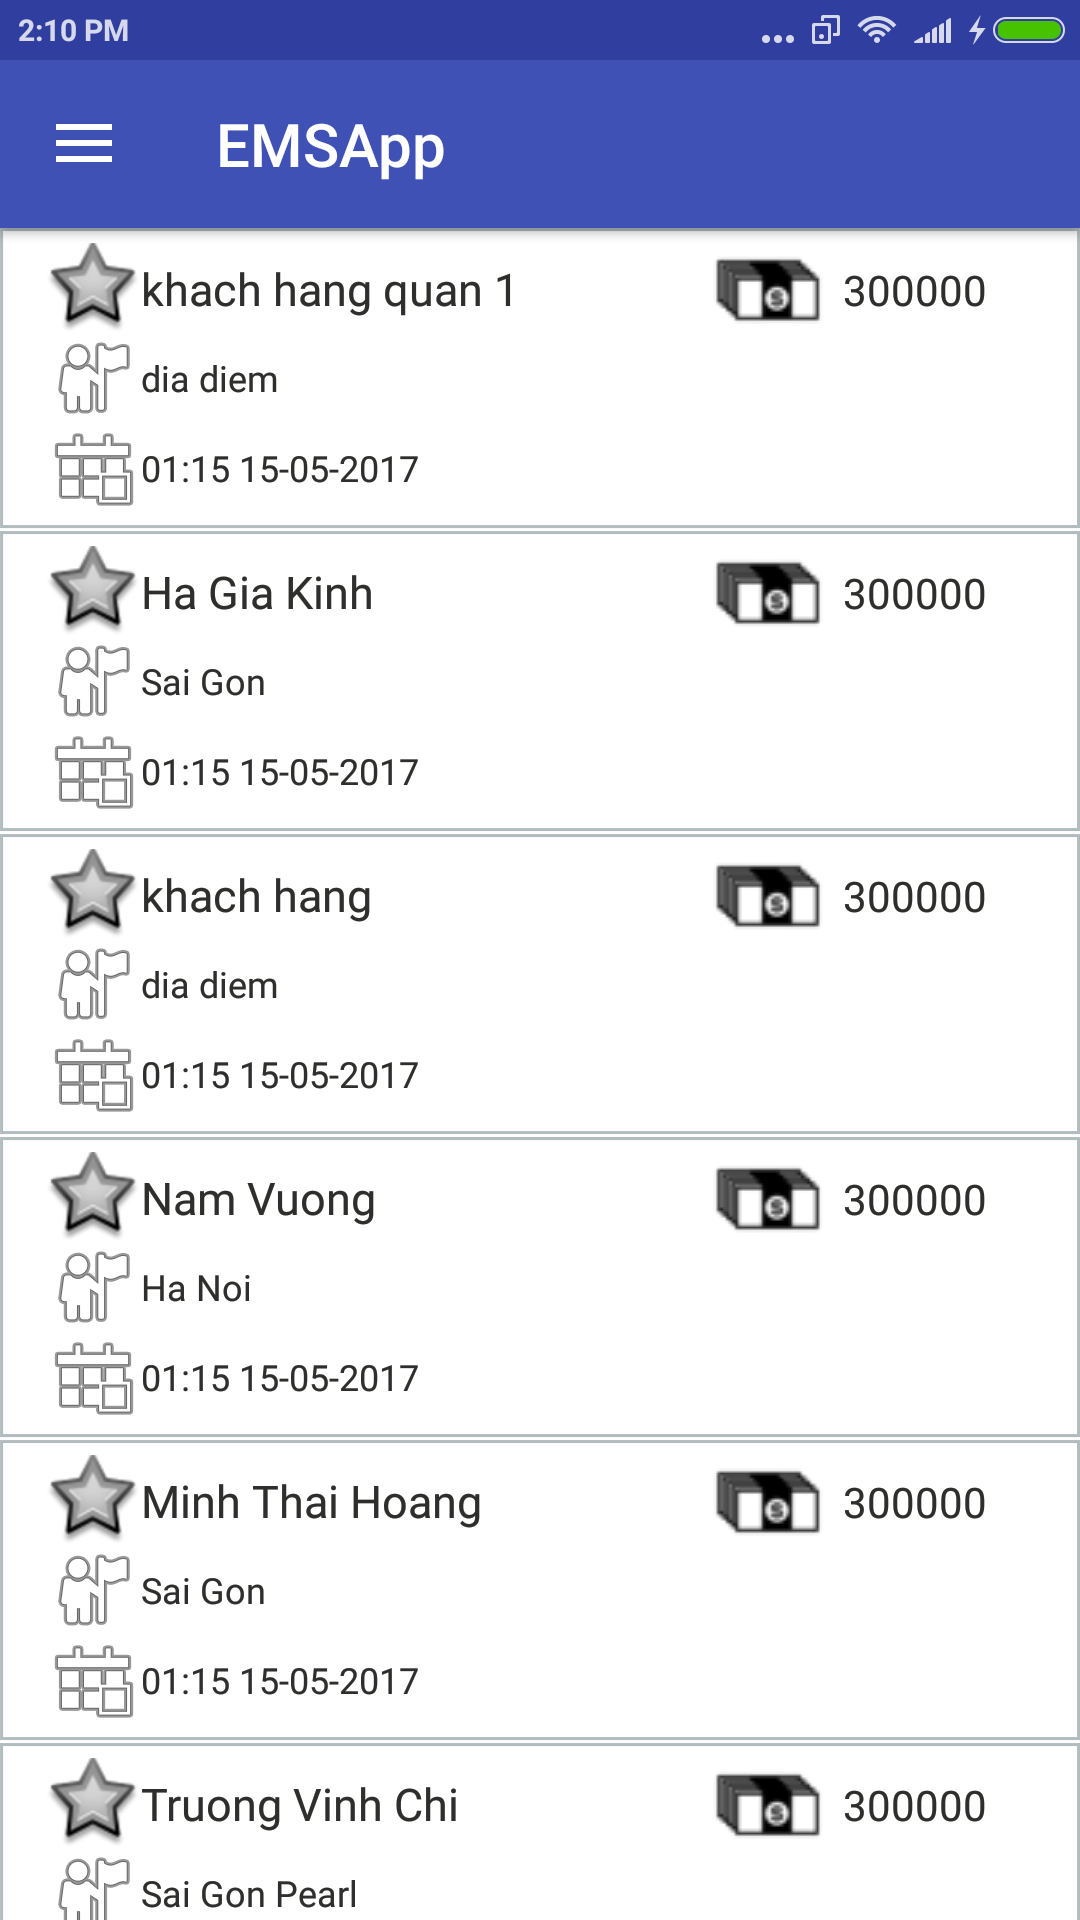
\includegraphics[scale=0.08]{/Client/UI/finished-appointment}} 
    \centering
    \caption{Màn hình danh sách lịch sử các cuộc hẹn đã hoàn thành}
    \label{fig:ui_employee_list}
\end{figure} 
\\
\textbf{Màn hình thông tin người dùng}\\\\
Người dùng có thể dễ dàng xem thông tin cá nhân của mình thông qua chức năng User Info.\\\\
Tại đây người dùng có thể chọn thay đổi mật khẩu nếu cần thiết.\\
\begin{figure}[!h]
  \fbox{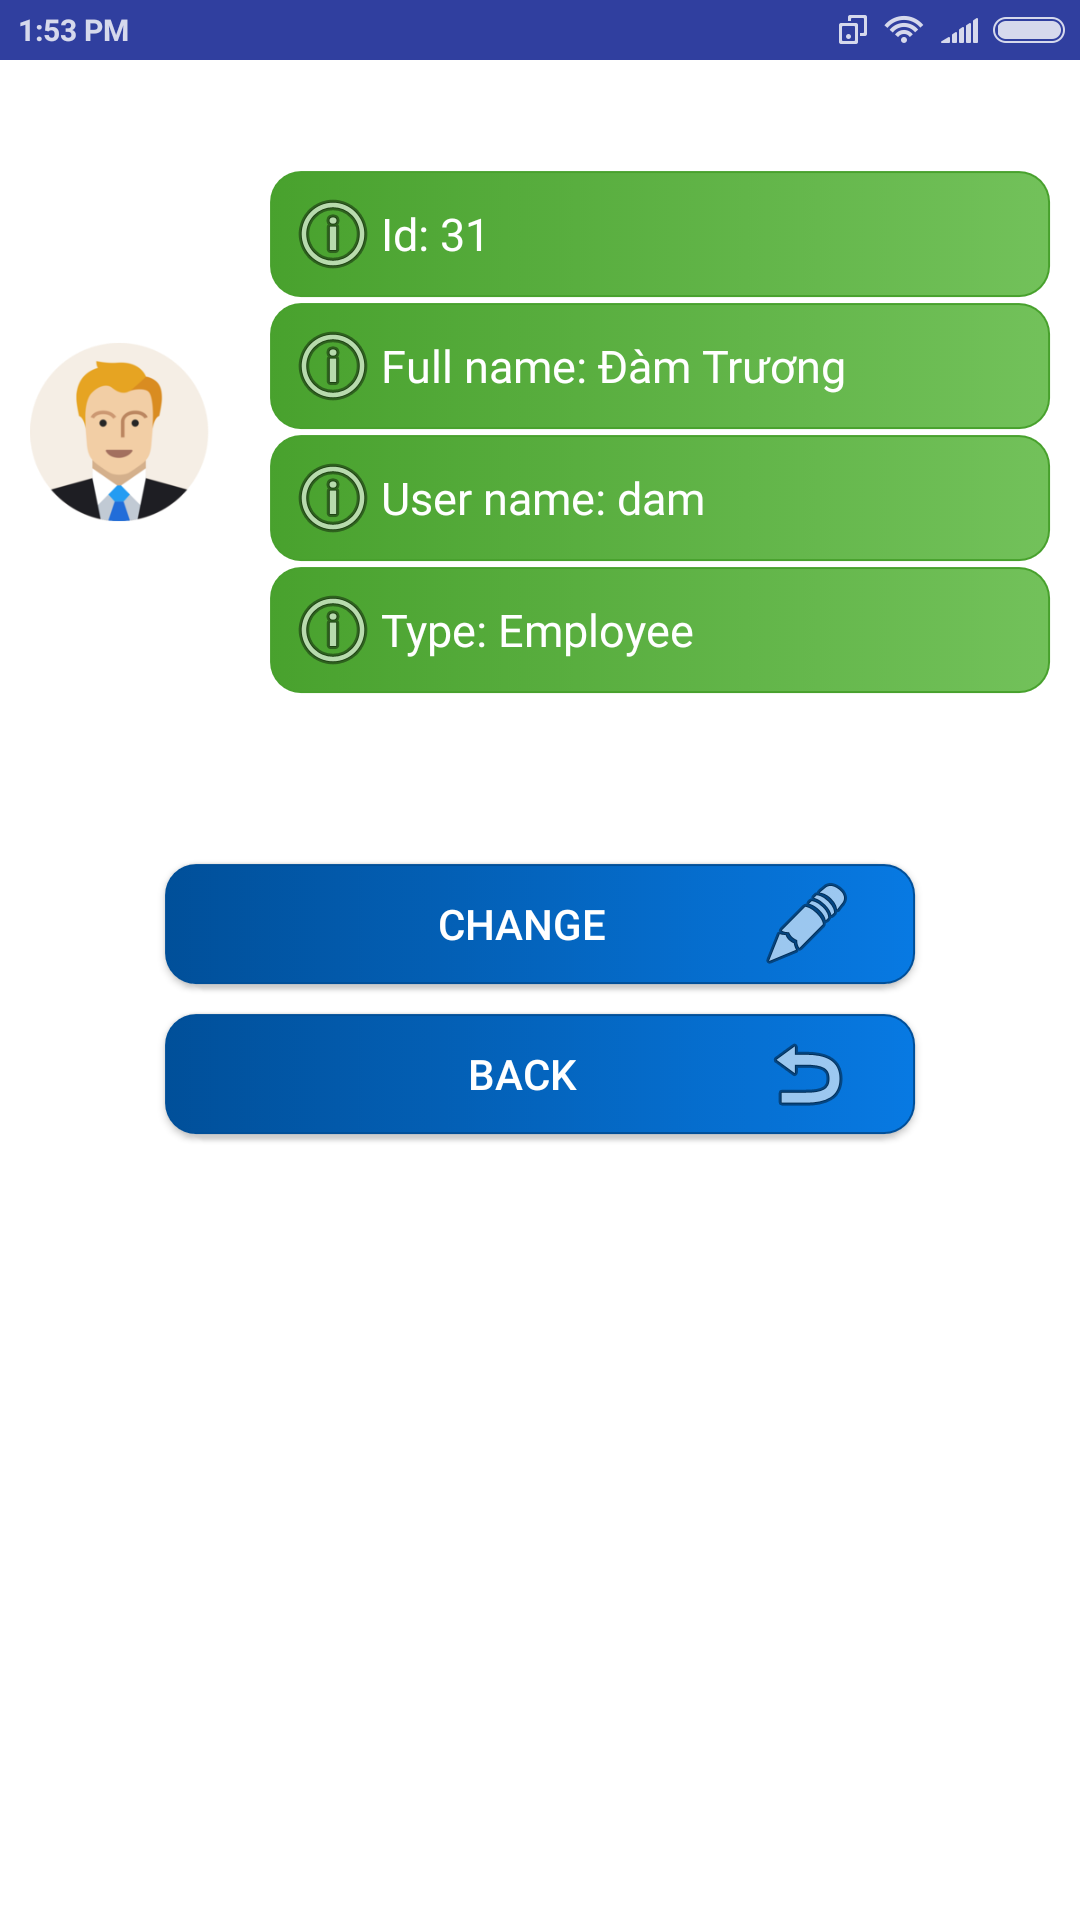
\includegraphics[scale=0.08]{/Client/UI/user-info}} 
    \centering
    \caption{Màn hình thông tin người dùng}
    \label{fig:ui_employee_list}
\end{figure} 
\\
\textbf{Màn hình đổi mật khẩu}\\\\
Người dùng nhập mật khẩu hiện tại, mật khẩu mới và xác nhận lại mật khẩu mới thêm một lần nữa.  Sau đó chọn nút Save để lưu thay đổi.\\
\begin{figure}[!h]
  \fbox{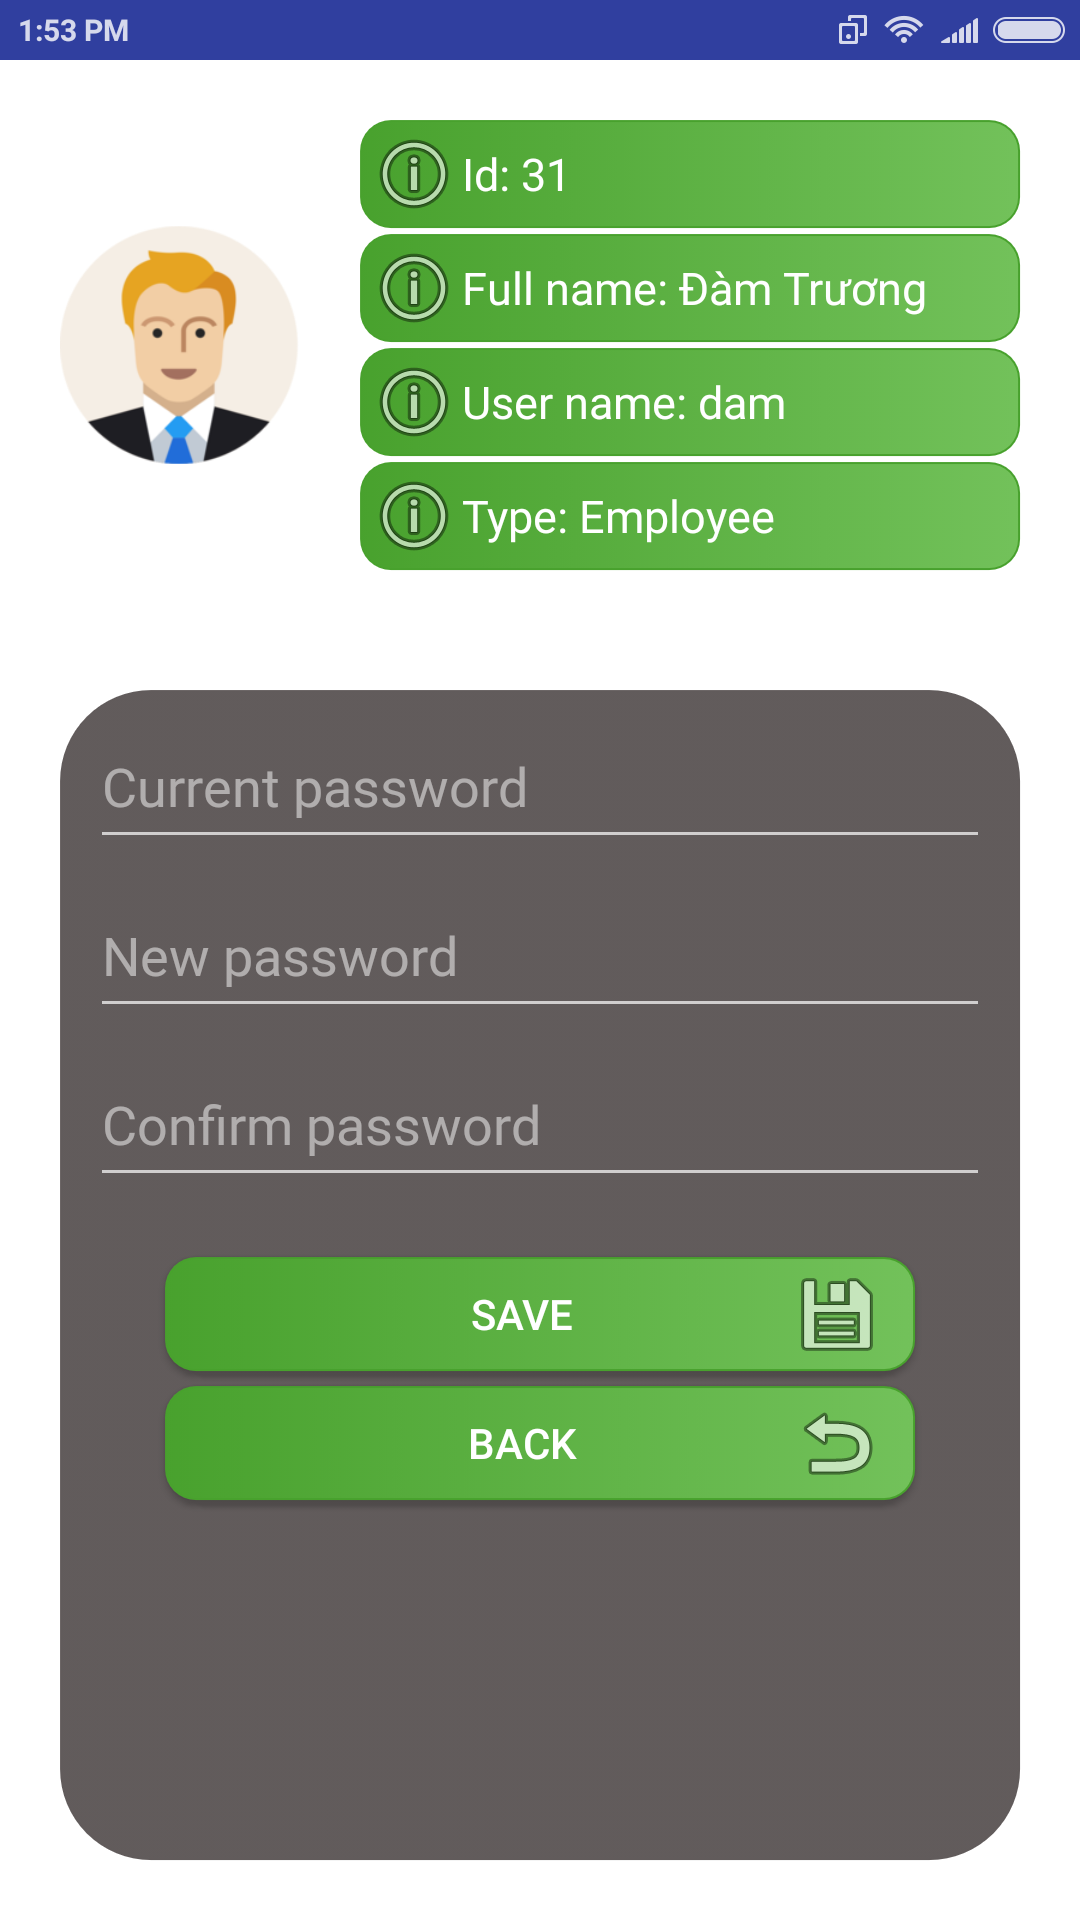
\includegraphics[scale=0.1]{/Client/UI/change-password}} 
    \centering
    \caption{Màn hình đổi mật khẩu}
    \label{fig:ui_employee_list}
\end{figure} 
\\
\\
\textbf{Màn hình tạo mới một lịch trình}\\\\
Đối với người dùng là quản lý, người dùng sẽ có thêm chức năng tạo mới một cuộc hẹn.\\\\
Để tạo mới một cuộc hẹn, người dùng sẽ cung cấp cho hệ thống một số thông tin cơ bản bao gồm tên cuộc hẹn, địa điểm hẹn, thời điểm và danh sách các nhân viên được gán cho cuộc hẹn đó.\\\\
Cuối cùng chọn nút Save để tạo mới một cuộc hẹn.\\
\begin{figure}[!h]
  \fbox{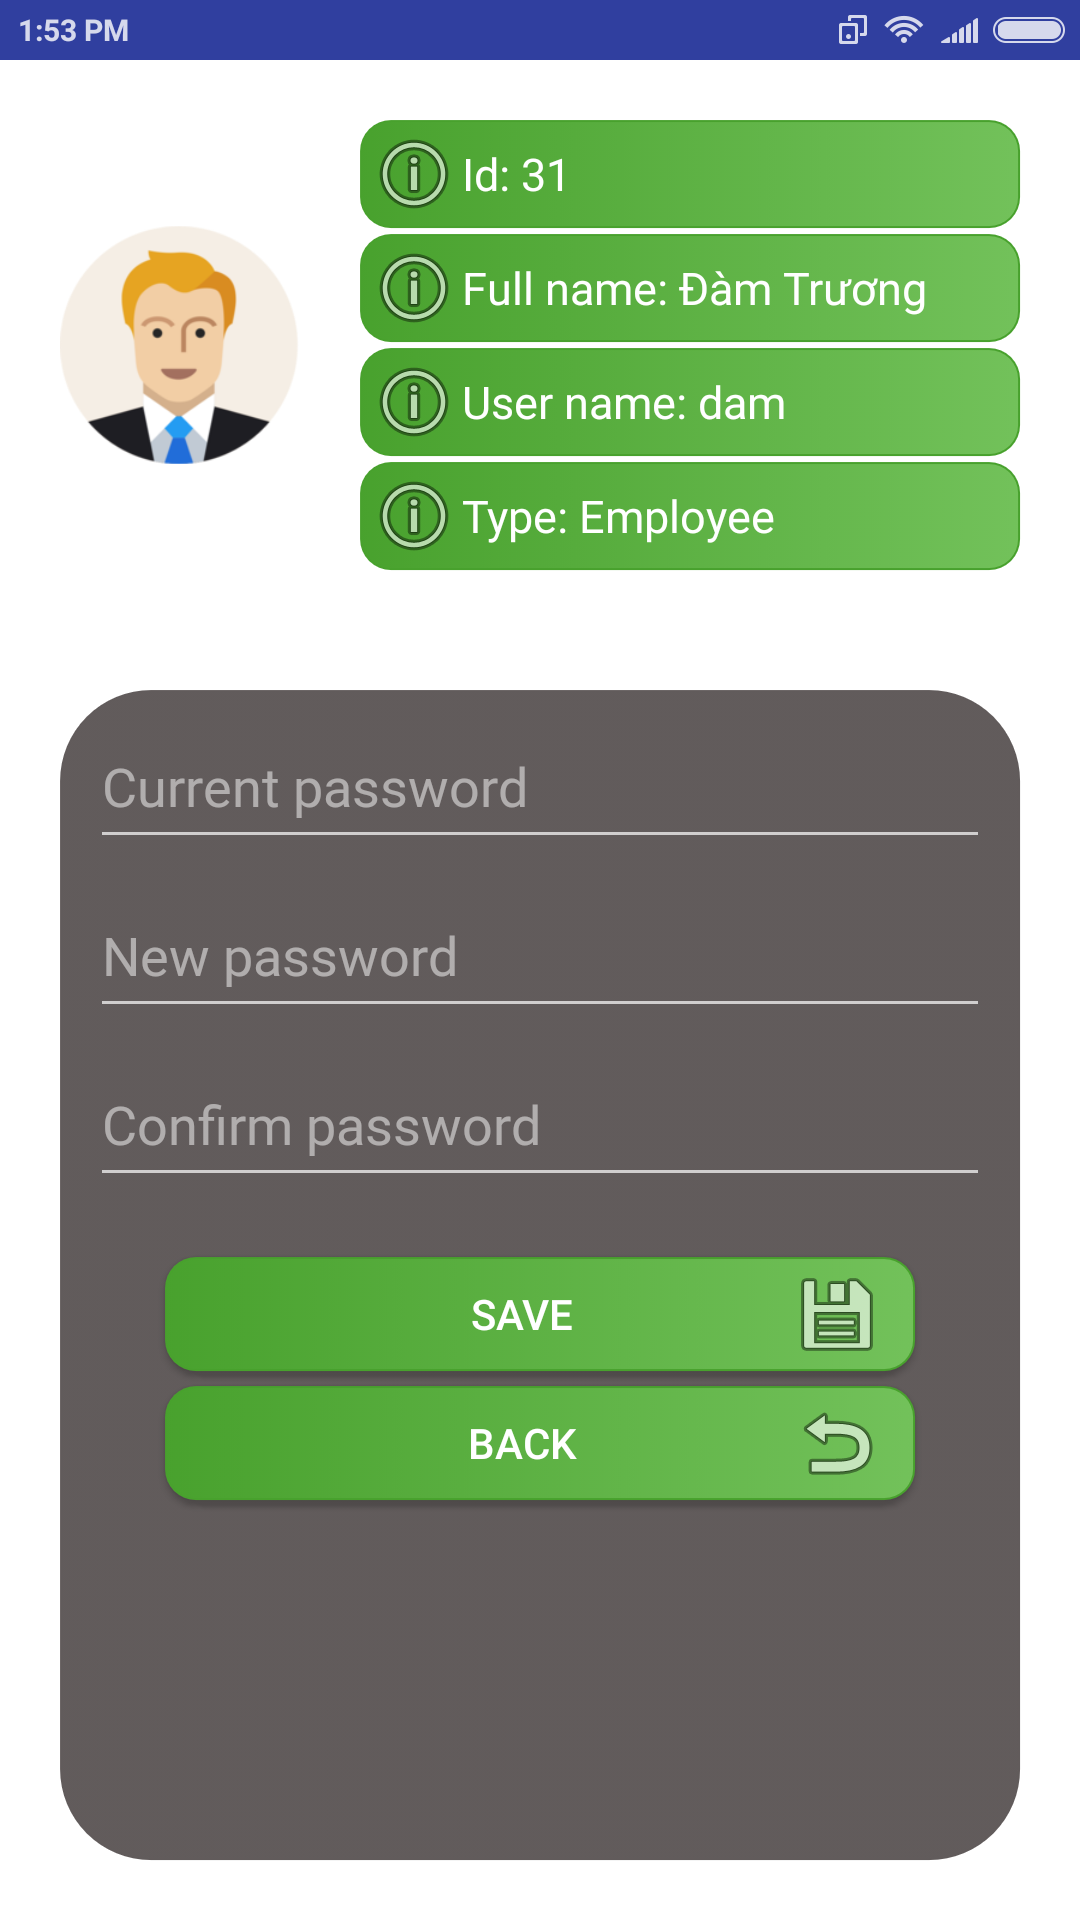
\includegraphics[scale=0.1]{/Client/UI/change-password}} 
    \centering
    \caption{Màn hình tạo một cuộc hẹn}
    \label{fig:ui_employee_list}
\end{figure} 
\\
\begin{figure}[!h]
  \fbox{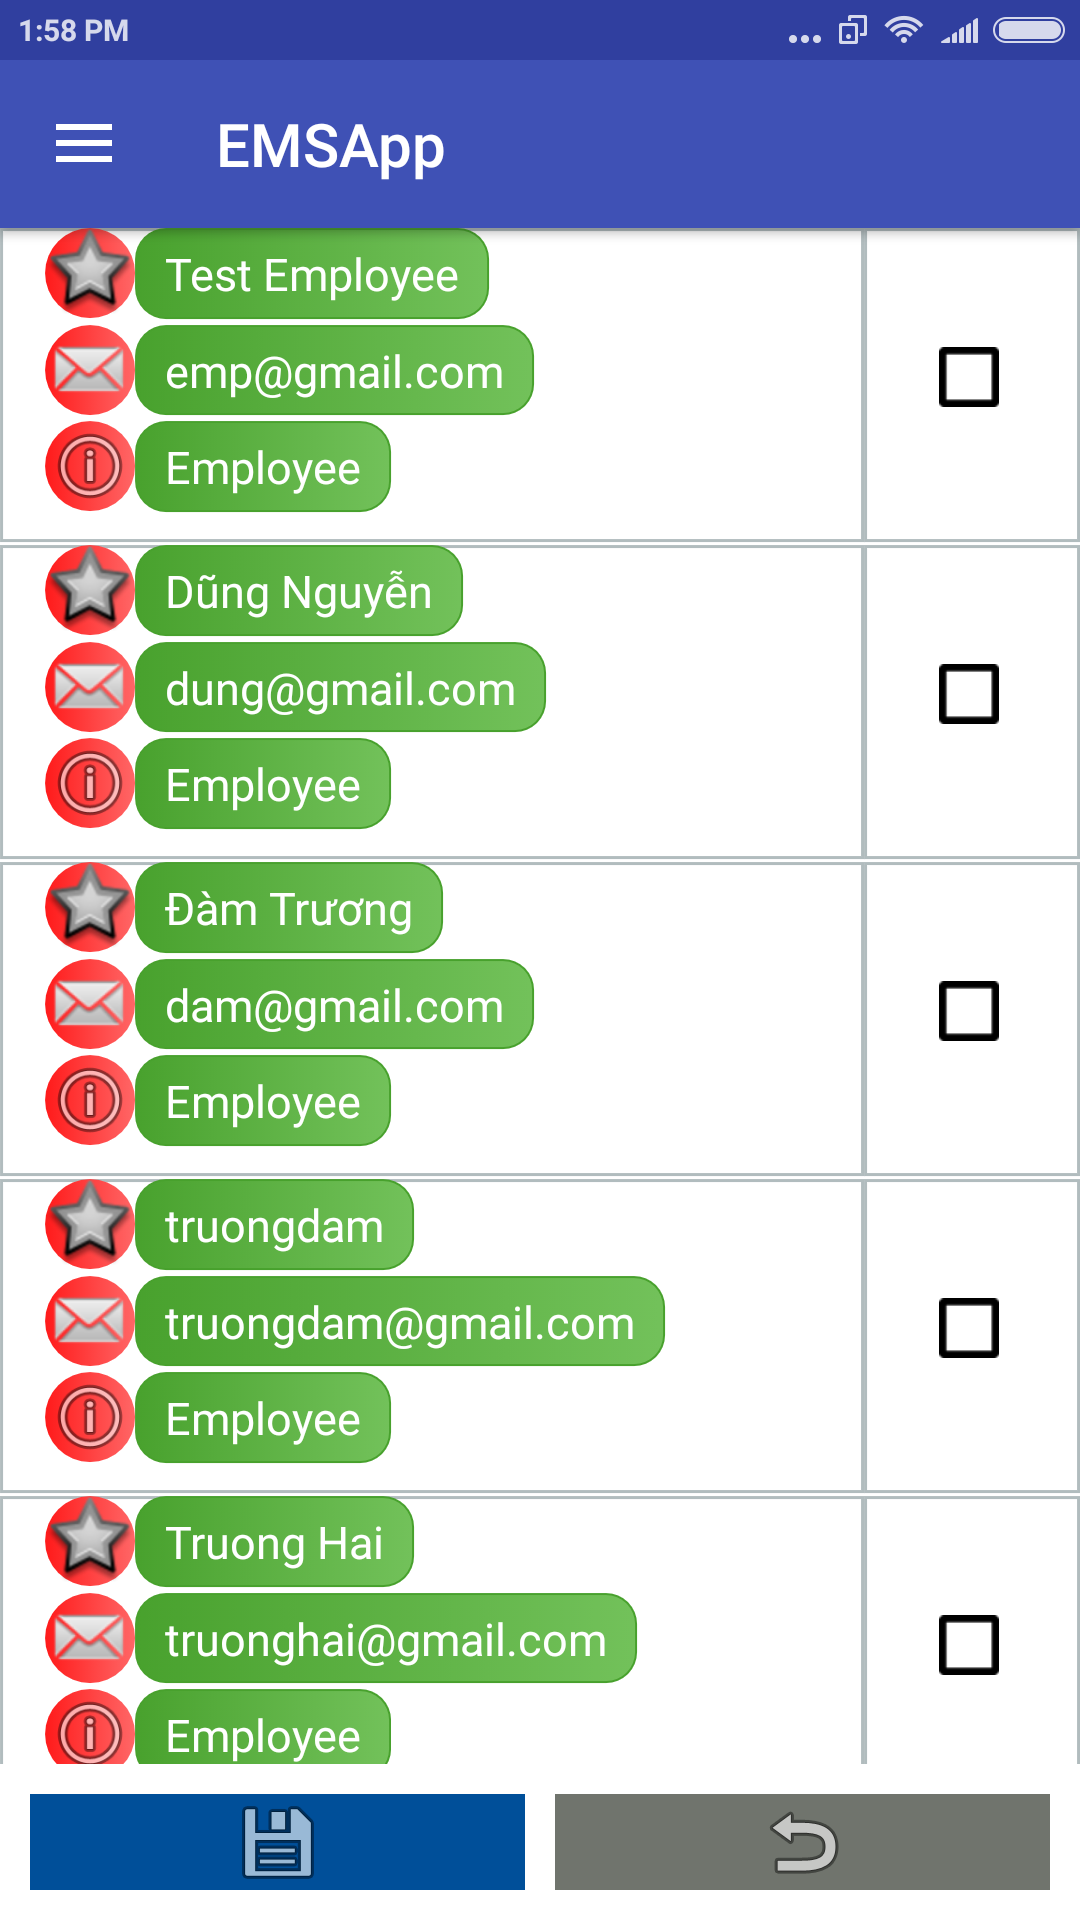
\includegraphics[scale=0.1]{/Client/UI/choose-employee}} 
    \centering
    \caption{Màn hình chọn nhân viên cho cuộc hẹn}
    \label{fig:ui_employee_list}
\end{figure} 
\\
\clearpage
\noindent
\textbf{Màn hình danh sách khách hàng}\\\\
Ngoài ra người quản lý còn có một màn hình riêng để quản lý danh sách các khách hàng của mình.\\\\
Một số thông tin cơ bản của khách hàng bao gồm họ tên, email, số điện thoại.\\
\begin{figure}[!h]
  \fbox{\includegraphics[scale=0.1]{/Client/UI/client-list}} 
    \centering
    \caption{Màn hình danh sách khách hàng}
    \label{fig:ui_employee_list}
\end{figure} 
\subsection{Server}
%\subsubsection{Thiết kế bản kiểm thử}
%\textbf{Chức năng đăng nhập hệ thống}
%\begin{table}[!h]
%    \centering
%    \begin{tabular}{|m{3.4cm}|m{4.2cm}|m{4.2cm}|c|c|}
%    \hline
%    \thead{Testcase} & \thead{Bước thực hiện} & \thead{Kết quả đạt được}& \thead{Đã kiểm\\ tra?} & \thead{Đạt?}\\\hline
%    Đăng nhập vào hệ thống với hai trường username và password đều trống&\pbox{4.2cm}{1) Truy cập vào đường dẫn trang web.\\
%2) Bỏ trống cả hai trường username và password.\\
%3) Bấm vào nút “LOGIN”}&\pbox{4.2cm}{Hệ thống sẽ trả về lỗi : \\- username cannot be empty and must be within 4 to 32 characters\\- password cannot be empty and must be within 4 to 32 characters\\}&\checkmark&\checkmark\\\hline
%Đăng nhập vào hệ thống với một trong hai trường bị bỏ trống.&\pbox{4.2cm}{1) Truy cập vào đường dẫn trang web. \\
%2) Bỏ trống một trong hai trường username hoặc password. \\
%3) Bấm vào nút “LOGIN”
%}&\pbox{4.2cm}{Hệ thống sẽ trả về lỗi : \\
%- Nếu ta bỏ trống trường username : username cannot be empty and must be within 4 to 32 characters\\
%- Nếu ta bỏ trống trường password : password cannot be empty and must be within 4 to 32 characters \\
%}&\checkmark&\checkmark\\\hline
%Đăng nhập vào hệ thống với cả hai trường username và password có độ dài bé hơn 4 hoặc lớn hơn 32 ký tự&\pbox{4.2cm}{1) Truy cập vào đường dẫn trang web. \\
%2) Nhập vào trường username và password giá trị “abc”. \\
%3) Bấm vào nút “LOGIN”
%}&\pbox{4.2cm}{Hệ thống sẽ trả về lỗi : \\
%- username cannot be empty and must be within 4 to 32 characters\\
%- password cannot be empty and must be within 4 to 32 characters\\
%}&\checkmark&\checkmark\\\hline
%    \end{tabular}
%    \caption{Choose a vehicle}
%\end{table}
%\subsubsection{Danh sách các hàm được sử dụng}
%\begin{longtable}{|m{3cm}|m{3.6cm}|m{6.8cm}|}
%    \hline
%    \thead{Tên hàm} & \thead{Chức năng} & \thead{Thông số đầu vào}\\\hline
%\texttt{CreateAppointment}&Tạo một công tác và lưu vào trong cơ sở dữ liệu.&\pbox{6.8cm}{Một JSON Object bao gôm các trường: \\- \texttt{destination}: đích đến của công tác (Chuỗi). \\- \texttt{start\_date}: ngày bắt đầu dự kiến của công tác(Chuỗi  có dạng HH:mm dd-MM-yyyy).\\- \texttt{users}: danh sách mã số những người tham gia công tác (Chuỗi có dạng 1,2,3,4).\\- \texttt{client\_id}: mã số của khách hàng đã được lưu trong cơ sở dữ liệu (Số  nguyên). }\\\hline
%\texttt{\pbox{3cm}{GetActiveAppoint-\\ments}}&Lấy danh sách các công tác chưa kết thúc trong cơ sở dữ liệu.&không có tham số nào. \\\hline
%\texttt{\pbox{3cm}{GetCompletedAppo-\\intments}}&Lấy danh sách các công tác đã kết thúc trong cơ sở dữ liệu.&không có tham số nào. \\\hline
%\texttt{UpdateAppointment}&Cập nhật thông tin một công tác đã tồn tại trong cơ sở dữ liệu (chỉ dùng cho người quản lý).& \pbox{6.8cm}{Một JSON Object bao gôm các trường:\\
%- \texttt{destination}: đích đến của công tác (Chuỗi).\\- \texttt{start\_date}: ngày bắt đầu dự kiến của công tác (Chuỗi  có dạng HH:mm dd-MM-yyyy).\\- \texttt{users}: danh sách mã số những người tham gia công tác (Chuỗi có dạng 1,2,3,4).\\- \texttt{client\_id}: mã số của khách hàng đã được lưu trong cơ sở dữ liệu (Số nguyên).\\- \texttt{appointment\_id}: mã số của công tác ta muốn cập nhật (Số nguyên). \\
%}\\\hline
%\texttt{EndAppointment}&Kết thúc một công tác và cập nhật vào cơ sở dữ liệu.& \pbox{6.8cm}{Một JSON Object bao gôm các trường\\- \texttt{id}: mã số của công tác (Số nguyên).\\- \texttt{end\_date}: thời gian kết thúc của công tác (Chuỗi có dạng HH:mm dd-MM-yyyy).}\\\hline
%\texttt{CreateClient}&Tạo một khách hàng và lưu vào trong cơ sở dữ liệu.& \pbox{6.8cm}{Một JSON Object bao gôm các trường:\\- \texttt{name}: tên của khách hàng (Chuỗi). \\ 
%- \texttt{phone\_number}: số điện thoại của khách hàng (Chuỗi số bao gôm 10-11 số nhất và chỉ được thêm khoảng trắng).\\
%- \texttt{address}: địa chỉ của khách hàng (Chuỗi).\\
%- \texttt{email}:  email của khách hàng (Chuỗi tuân theo đúng định dạng email).\\ }\\\hline
%\texttt{GetClients}&Lấy danh sách các khách hàng đã lưu trong cơ sở dữ liệu.&không có thông số nào. \\\hline
%\texttt{GetClientInfo}&Lấy thông tin chi tiết của một khách hàng.&Một JSON Object chứa một trường duy nhất là mã số của khách hàng (Số nguyên). \\\hline
%\texttt{AddCoordinate}&Thêm một (hoặc nhiều) tọa độ vị trí cho một lịch trình.& \pbox{6.8cm}{Một JSON Object bao gôm các trường:\\
%- \texttt{detail\_id}: mã số của lịch trình.\\ 
%- \texttt{coordinates}: mảng các tọa độ (JSON Array) có cấu trúc của một phần tử bao gồm ba trường: latitude (vĩ độ - Số thực), longitude (kinh độ - số thực) và time (thời gian - chuỗi có dạng HH:mm:ss dd-MM-yyyy).\\}\\\hline
%\texttt{CreateDetail}&Tạo một lịch trình và lưu vào trong cơ sở dữ liệu, đồng thời ta cũng bắt đầu luôn lịch trình này.& \pbox{6.8cm}{
%Một JSON Object bao gôm các trường:\\
%- \texttt{vehicle\_id}: mã số của phương tiện (Số nguyên).\\ 
%- \texttt{start\_time}: thời gian bắt đầu của lịch trình (Chuỗi  có dạng HH:mm:ss dd-MM-yyyy).\\
%- \texttt{start\_location}: vị trí bắt đầu của lịch trình (Chuỗi có dạng 1,2,3,4).\\
%- \texttt{appointment\_id}: mã số của công tác đã được lưu trong cơ sở dữ liệu (Số  nguyên).\\ }  \\\hline
%\texttt{EndDetail}&Kết thúc một lịch trình.& \pbox{6.8cm}{Một JSON Object bao gôm các trường:\\
%- \texttt{image\_content}: hình ảnh hóa đơn được người dùng chụp lại, đây là một chuỗi có nội dung là base 64 của file hình ảnh, có thể rỗng.\\ 
%- \texttt{description}: ghi chú của lịch trình này (kẹt xe, bể bánh, thêm tiền, ...) (Chuỗi).\\
%- \texttt{input\_cost}: số tiền phải trả để thực hiện lịch trình (Số thực).\\}\\\hline
%\texttt{GetEmployees}&Lấy danh sách các nhân viên dưới quyền quản lý (chỉ dùng cho người quản lý).&Một JSON Object bao một trường duy nhất là mã số của người dùng (Số nguyên). \\\hline
%\texttt{GetUserInfo}&Lấy thông tin chi tiết của một người dùng.&Một JSON Object bao một trường duy nhất là mã số của người dùng (Số nguyên). \\\hline
%\texttt{GetVehicles}&Lấy danh sách các phương tiện đi lại.&không có tham số nào. \\\hline
%    \caption{Bảng các hàm chính được sử dụng của hệ thống.}
%\end{longtable}
\subsection{Phiên bản mẫu Server}
Sau đây nhóm xin trình bày một số phiên bản mẫu (phần còn lại vui lòng xem lại ở phụ lục phần 4) :
\subsubsection{Trang chủ của hệ thống}
Trang chủ của hệ thống hiển thị giao diện mà hệ thống hiện ra cho người quản trị sau khi người quản trị đăng nhập thành công. Người quản trị sẽ dùng menu hiện ra ở phía
bên tay trái để đi đến các trang web khác.

\begin{figure}[H]
\centering
\includegraphics[scale=0.5]{admin/admin_trangchu}
\caption{Màn hình trang chủ}
\end{figure}

\subsubsection{Trang thêm, cập nhật công thức dự đoán chi phi phương tiện}
Trang này dự cho phép người sử dụng thêm hoặc cập nhật lại một công thức dự đoán chi phí của một phương tiện dựa vào thời gian và quãng đường sử dụng phương tiện đó. Hiện
tại hệ thống hỗ trợ cho người dùng những phép toán cộng trừ nhân chia cơ bản.

\begin{figure}[H]
\centering
\includegraphics[scale=0.5]{admin/admin_chiphi}
\caption{Màn hình cập nhật công thức dự đoán chi phí phương tiện}
\end{figure}


\subsubsection{Chức năng quản lý của người quản trị}
Hiện thực tất cả các chức năng quản lý của người quản trị bao gồm quản lý người dùng, quản lý khách hàng, quản lý phương tiện, quản lý danh sách các vị trí đặc biệt.
Những hình bên dưới là phiên bản quản lý người dùng với các chức năng xem, tìm kiếm, sắp xếp, thêm, chỉnh sửa, vô hiệu hóa và thống kê.

\begin{figure}[H]
\centering
\includegraphics[scale=0.5]{admin/admin_employee}
\caption{Màn hình quản lí nhân viên}
\end{figure}


\begin{figure}[H]
\centering
\includegraphics[scale=0.5]{admin/admin_themnhanvien}
\caption{Màn hình quản lí thêm nhân viên}
\end{figure}

\begin{figure}[H]
\centering
\includegraphics[scale=0.5]{admin/admin_chinhsuanhanvien}
\caption{Màn hình quản lí chỉnh sửa thông tin nhân viên}
\end{figure}

\begin{figure}[H]
\centering
\includegraphics[scale=0.5]{admin/admin_lichtrinh}
\caption{Màn hình quản lí các lịch trình của nhân viên}
\end{figure}

\begin{figure}[H]
\centering
\includegraphics[scale=0.5]{admin/admin_lichtrinhchart}
\caption{Màn hình thể hiện các lịch trình của nhân viên theo biểu đồ}
\end{figure}
\subsection{Thiết kế bản kiểm thử (những chức năng chính)}
Sau đây nhóm xin trình bày một số phiên bản mẫu (phần còn lại vui lòng xem lại ở phụ lục phần 3) : 
\subsubsection {Chức năng đăng nhập vào hệ thống}

\begin{longtable}{ | p{.15\textwidth} |p{.30\textwidth} | p{.35\textwidth}  | p{.10\textwidth}  | p{.10\textwidth}  | } 
\hline
\textbf{Testcase}& \textbf{Bước thực hiện}& \textbf{Kết quả đạt được} & \textbf{Đã kiểm tra}& \textbf{Đạt} \\ 
\hline
\hline
Đăng nhập vào hệ thống với hai trường username và password đều trống &
Các bước thực hiện: \newline
- Truy cập vào đường dẫn trang web. \newline
- Bỏ trống cả hai trường username và password. \newline
- Bấm vào nút “LOGIN”
&
Hệ thống sẽ trả về lỗi : \newline
- username cannot be empty and must be within 4 to 32 characters. \newline
- password cannot be empty and must be within 4 to 32 characters.
&
Đã kiểm tra &
Đạt \\

\hline
Đăng nhập vào hệ thống với một trong hai trường bị bỏ trống. &
Các bước thực hiện: \newline
- Truy cập vào đường dẫn trang web. \newline
- Bỏ trống một trong hai trường username hoặc password.  \newline
- Bấm vào nút “LOGIN”. 
&
Hệ thống sẽ trả về lỗi : \newline
- Nếu ta bỏ trống trường username : username cannot be empty and must be within 4 to 32 characters. \newline
- Nếu ta bỏ trống trường password : password cannot be empty and must be within 4 to 32 characters . \newline
&
Đã kiểm tra &
Đạt \\

\hline
Đăng nhập vào hệ thống với cả hai trường username và password có độ dài bé hơn 4 hoặc lớn hơn 32 ký tự &
Các bước thực hiện: \newline
- Truy cập vào đường dẫn trang web. \newline
- Nhập vào trường username và password giá trị “abc”.  \newline
- Bấm vào nút “LOGIN”.
&
Hệ thống sẽ trả về lỗi : \newline
- username cannot be empty and must be within 4 to 32 characters. \newline
- password cannot be empty and must be within 4 to 32 characters. \newline
&
Đã kiểm tra &
Đạt \\

\hline
Đăng nhập vào hệ thống với trường username có độ dài bé hơn 4 ký tự và lớn hơn 32 ký tự &
Các bước thực hiện: \newline
- Truy cập vào đường dẫn trang web.  \newline
- Nhập vào trường username giá trị “abcd” và password giá trị “abcdefgh”.  \newline
- Bấm vào nút “LOGIN”.
&
Hệ thống sẽ trả về lỗi : \newline
username cannot be empty and must be within 4 to 32 characters \newline
&
Đã kiểm tra &
Đạt \\


\hline
Đăng nhập vào hệ thống với trường password có độ dài bé hơn 4 ký tự và lớn hơn 32 ký tự &
Các bước thực hiện: \newline
- Truy cập vào đường dẫn trang web. \newline
- Nhập vào trường username giá trị “abcdefgh” và password giá trị “abd”. \newline
- Bấm vào nút “LOGIN”.
 &
Hệ thống sẽ trả về lỗi : \newline
- password cannot be empty and must be within 4 to 32 characters.
 &
Đã kiểm tra &
Đạt \\

\hline
Đăng nhập vào hệ thống với hai (hoặc một trong hai) trường username và password sai  &
Các bước thực hiện: \newline
- Truy cập vào đường dẫn trang web. \newline
- Nhập vào trường username giá trị “admin” và password giá trị “admin1”.  \newline
- Bấm vào nút “LOGIN”
&
Hệ thống sẽ trả về lỗi : Invalid username or password.
&
Đã kiểm tra &
Đạt \\

\hline
Đăng nhập vào hệ thống với cả hai trường username và password đã tồn tại trong database &
Các bước thực hiện: \newline
- Truy cập vào đường dẫn trang web. \newline
- Nhập vào trường username giá trị “admin” và password giá trị “admin”.  \newline
- Bấm vào nút “LOGIN”
&
Hệ thống sẽ đưa ta đến trang chủ. Đăng nhập thành công. &
Đã kiểm tra &
Đạt \\
\hline
\caption{Bảng kiểm thử đăng nhập vào hệ thống}
\end{longtable}

\subsubsection{Thao tác đối với trang Lịch trình (Appointments)}
\begin{longtable}{ | p{.15\textwidth} |p{.30\textwidth} | p{.35\textwidth}  | p{.10\textwidth}  | p{.10\textwidth}  | } 
\hline
\textbf{Testcase}& \textbf{Bước thực hiện}& \textbf{Kết quả đạt được} & \textbf{Đã kiểm tra}& \textbf{Đạt} \\ 
\hline
\hline
Kiểm tra chức năng cho phép người dùng chọn trạng thái của lịch trình &
Các bước thực hiện: \newline
- Chọn dropdown list nằm ở dưới nhãn : “Select the status of appointments:”. \newline
- Thay đổi giá trị của dropdown list này (giá trị mặc định đang là “View all”).
&
Hệ thống sẽ trả về danh sách các lịch trình có trạng thái (Status) tương ứng với giá trị dropdown list mà ta vừa đổi. &
Đã kiểm tra &
Đạt \\

\hline
Kiểm tra chức năng tìm kiếm của bảng dữ liệu &
Các bước thực hiện: \newline
- Chọn ô tìm kiếm trong bảng dữ liệu. \newline
- Nhập vào một giá trị nào đó. 
&
Dữ liệu trong bảng sẽ thay đổi, hệ thống sẽ chỉ hiện ra những lịch trình có liên quan đến từ khóa ta nhập vào. &
Đã kiểm tra &
Đạt \\

\hline
Kiểm tra chức năng tìm kiếm theo từng cột của bảng dữ liệu &
Các bước thực hiện:
Chọn một cột trong bảng dữ liệu. \newline
- Bấm vào tên của cột đó.  \newline
&
Dữ liệu trong bảng sẽ được sắp xếp lại theo giá trị của cột ta đã chọn theo chiều tăng dần hoặc giảm dần. &
Đã kiểm tra &
Đạt \\

\hline
Kiểm tra chức năng paging của bảng &
Các bước thực hiện: \newline
- Chọn dropdown list nằm ngang với nhãn “Show...entries:”.  \newline
- Giá trị mặc định là 10 hàng một trang, ta tiến hành đổi giá trị này. Nếu số trang của bảng dữ liệu lớn hơn một, ta tiến hành bầm các nút “Previous”,”Next” hoặc bấm vào số thứ tự của trang.
&
Hệ thống sẽ trả về dữ liệu tương ứng với những giá trị ta thay đổi. &
Đã kiểm tra &
Đạt \\


\hline
Kiểm tra thông tin chi tiết của một lịch trình &
Các bước thực hiện: \newline
-  Chọn một lịch trình trong bảng dữ liệu. \newline
-  Bấm vào nút “Details” tương ứng với lịch trình đó (nút này sẽ nàm cùng hàng với lịch trình). &
Hệ thống sẽ đưa ta đến trang thông tin chi tiết của lịch trình.&
Đã kiểm tra &
Đạt \\

\hline
\caption{Bảng kiểm thử thao tác trang Lịch trình}
\end{longtable}

%Managers 
\subsubsection{Thao tác đối với trang Người quản lý  (Managers)}
\begin{longtable}{ | p{.15\textwidth} |p{.30\textwidth} | p{.35\textwidth}  | p{.10\textwidth}  | p{.10\textwidth}  | } 
\hline
\textbf{Testcase}& \textbf{Bước thực hiện}& \textbf{Kết quả đạt được} & \textbf{Đã kiểm tra}& \textbf{Đạt} \\ 
\hline
\hline
Kiểm tra chức năng cho phép người dùng thêm người quản lý mới &
Các bước thực hiện: \newline
- Bấm vào nút “ADD NEW MANAGER.
&
Hệ thống sẽ đưa người dùng đến trang thêm người quản lý mới. &
Đã kiểm tra &
Đạt \\

\hline
Kiểm tra chức năng tìm kiếm của bảng dữ liệu. &
Các bước thực hiện: \newline
- Chọn ô tìm kiếm trong bảng dữ liệu. \newline
- Nhập vào một giá trị nào đó. 
&
Dữ liệu trong bảng sẽ thay đổi, hệ thống sẽ chỉ hiện ra những lịch trình có liên quan đến từ khóa ta nhập vào. &
Đã kiểm tra &
Đạt \\

\hline
Kiểm tra chức năng tìm kiếm theo từng cột của bảng dữ liệu. &
Các bước thực hiện: \newline
- Chọn một cột trong bảng dữ liệu.  \newline
- Bấm vào tên của cột đó. 
&
Dữ liệu trong bảng sẽ được sắp xếp lại theo giá trị của cột ta đã chọn theo chiều tăng dần hoặc giảm dần. &
Đã kiểm tra &
Đạt \\

\hline
Kiểm tra chức năng paging của bảng. &
Các bước thực hiện: \newline
- Chọn dropdown list nằm ngang với nhãn "Show...entries:".   \newline
- Giá trị mặc định là 10 hàng một trang, ta tiến hành đổi giá trị này. \newline
- Nếu số trang của bảng dữ liệu lớn hơn một, ta tiến hành bầm các nút “Previous”,”Next” hoặc bấm vào số thứ tự của trang.
&
Hệ thống sẽ trả về dữ liệu tương ứng với những giá trị ta thay đổi. &
Đã kiểm tra &
Đạt \\

\hline
Kiểm tra thông tin chi tiết của một người quản lý. &
Các bước thực hiện: \newline
- Chọn một người quản lý trong bảng dữ liệu.    \newline
- Ta bấm vào nút “Details” tương ứng với người quản lý đó (nút này sẽ nằm cùng hàng với người quản lý).  
&
Hệ thống sẽ đưa ta đến trang thông tin chi tiết của người quản lý. &
Đã kiểm tra &
Đạt \\

\hline
Kiểm tra chức năng cập nhật lại thông tin của nhà quản lý. &
Các bước thực hiện: \newline
- Chọn một người quản lý trong bảng dữ liệu.     \newline
- Ta bấm vào nút “Update” tương ứng với người quản lý đó (nút này sẽ nằm cùng hàng với người quản lý). 
&
Hệ thống sẽ đưa ta đến trang cập nhật thông tin của người quản lý. &
Đã kiểm tra &
Đạt \\

\hline
\caption{Bảng kiểm thử thao tác trang Người quản lý}
\end{longtable}


%Employees 
\subsubsection{Thao tác đối với trang Nhân viên (Employees)}
\begin{longtable}{ | p{.15\textwidth} |p{.30\textwidth} | p{.35\textwidth}  | p{.10\textwidth}  | p{.10\textwidth}  | } 
\hline
\textbf{Testcase}& \textbf{Bước thực hiện}& \textbf{Kết quả đạt được} & \textbf{Đã kiểm tra}& \textbf{Đạt} \\ 
\hline
\hline
Kiểm tra chức năng cho phép người dùng thêm nhân viên mới. &
Các bước thực hiện: \newline
- Bấm vào nút “ADD NEW EMPLOYEE”. 
&
Hệ thống sẽ đưa người dùng đến trang thêm nhân viên mới. &
Đã kiểm tra &
Đạt \\

\hline
Kiểm tra chức năng tìm kiếm của bảng dữ liệu. &
Các bước thực hiện: \newline
- Chọn ô tìm kiếm trong bảng dữ liệu. \newline
- Nhập vào một giá trị nào đó. 
&
Dữ liệu trong bảng sẽ thay đổi, hệ thống sẽ chỉ hiện ra những lịch trình có liên quan đến từ khóa ta nhập vào. &
Đã kiểm tra &
Đạt \\

\hline
Kiểm tra chức năng sắp xếp theo từng cột của bảng dữ liệu. &
Các bước thực hiện: \newline
- Chọn một cột trong bảng dữ liệu.  \newline
- Bấm vào tên của cột đó. 
&
Dữ liệu trong bảng sẽ được sắp xếp lại theo giá trị của cột ta đã chọn theo chiều tăng dần hoặc giảm dần. &
Đã kiểm tra &
Đạt \\

\hline
Kiểm tra chức năng paging của bảng. &
Các bước thực hiện: \newline
- Chọn dropdown list nằm ngang với nhãn "Show...entries:".  \newline
- Giá trị mặc định là 10 hàng một trang, ta tiến hành đổi giá trị này. \newline
- Nếu số trang của bảng dữ liệu lớn hơn một, ta tiến hành bầm các nút "Previous","Next" hoặc bấm vào số thứ tự của trang. 
&
Hệ thống sẽ trả về dữ liệu tương ứng với những giá trị ta thay đổi. &
Đã kiểm tra &
Đạt \\

\hline
Kiểm tra thông tin chi tiết của một nhân viên. &
Các bước thực hiện: \newline
- Chọn một nhân viên trong bảng dữ liệu.   \newline
- Ta bấm vào nút “Details” tương ứng với nhân viên đó (nút này sẽ nằm cùng hàng với nhân viên). 
&
Hệ thống sẽ đưa ta đến trang thông tin chi tiết của nhân viên. &
Đã kiểm tra &
Đạt \\

\hline
Kiểm tra chức năng cập nhật lại thông tin của nhân viên. &
Các bước thực hiện: \newline
- Chọn một nhân viên trong bảng dữ liệu.    \newline
- Ta bấm vào nút “Update” tương ứng với nhân viên đó (nút này sẽ nằm cùng hàng với nhân viên). 
&
Hệ thống sẽ đưa ta đến trang cập nhật thông tin của nhân viên. &
Đã kiểm tra &
Đạt \\

\hline
\caption{Bảng kiểm thử thao tác trang Nhân viên}
\end{longtable}

%Employee Statistics 
\subsubsection{Thao tác khi sử dụng trang thống kê Nhân viên (Employee Statistics) }
Điều kiện ban đầu : Trang web hiển thị cho ta tất cả những thông tin đã được lưu trữ về nhân viên này, gười dùng có thể xem các lịch trình mà nhân viên này đã thực hiện trong một khoảng thời gian (theo tháng/năm), đồng thời thống kê số lượng lịch trình mà nhân viên đã đi dưới dạng biểu đồ. \newline
\begin{longtable}{ | p{.15\textwidth} |p{.30\textwidth} | p{.35\textwidth}  | p{.10\textwidth}  | p{.10\textwidth}  | } 
\hline
\textbf{Testcase}& \textbf{Bước thực hiện}& \textbf{Kết quả đạt được} & \textbf{Đã kiểm tra}& \textbf{Đạt} \\ 
\hline
\hline
Bỏ trống một trường dữ liệu. &
Các bước thực hiện: \newline
- Ta để trống cả trường dữ liệu nằm duới nhãn "Please input a year". \newline
- Bấm vào nút "View as chart" hoặc "View as list".
&
Hệ thống sẽ báo lỗi : Please input year value.
 &
Đã kiểm tra &
Đạt \\

\hline
Nhập sai kiểu dữ liệu cho trường dữ liệu. &
Các bước thực hiện: \newline
- Nhập giá trị “abc” vào trường dữ liệu nằm duới nhãn “Please input a year”. \newline
- Bấm vào nút “View as chart” hoặc “View as list”.
&
Hệ thống sẽ không cho người dùng nhập giá trị này, chỉ có giá trị số mới được nhận thôi.
 &
Đã kiểm tra &
Đạt \\

\hline
Thay đổi giá trị của dropdown list nằm dưới nhãn "Select period". &
Các bước thực hiện: \newline
- Chọn dropdown list nằm dưới nhãn "Select period". \newline
- Giá trị mặc định đang là "By months within a year". \newline
- Thay đổi giá trị của list này thành "By many years".
&
Giao diện trang web sẽ thay đổi : sẽ xuất hiện hai nhãn và hai trường dữ liệu tương ứng mới.
 &
Đã kiểm tra &
Đạt \\

\hline
\caption{Bảng kiểm thử thao tác trang thống kê Nhân viên}
\end{longtable}

%Formulas 
\subsubsection{Thao tác khi sử dụng trang thêm công thức cho Phương tiện (Insert Vehicle Formula) }
Điều kiện ban đầu : Trang web hiển thị cho ta 3 nút đó là Add formula, Add variable và Submit , người dùng phải nhập ít nhất một công thức thì mới có thể bấm nút Submit được , điều kiện để áp dụng các nguyên tắc phải tuân theo nguyên tắc sau : Nếu chỉ có một công thức được áp dụng cho mọi trường hợp, thì người dùng sẽ chọn Condition Type là “no condition”.  \newline
\begin{longtable}{ | p{.15\textwidth} |p{.30\textwidth} | p{.35\textwidth}  | p{.10\textwidth}  | p{.10\textwidth}  | } 
\hline
\textbf{Testcase}& \textbf{Bước thực hiện}& \textbf{Kết quả đạt được} & \textbf{Đã kiểm tra}& \textbf{Đạt} \\ 
\hline
\hline
Kiểm tra chức năng của nút Add formula. &
Các bước thực hiện: \newline
- Bấm vào nút Add formula.
&
Màn hình sẽ hiện ra thêm một đơn nhỏ bao gồm 3 trường Type, Condition và Formula. Nhiệm vụ của đơn này chính là để người dùng nhập công thức và điều kiện tương ứng của nó. &
Đã kiểm tra &
Đạt \\

\hline
Kiểm tra chức năng của nút Add variable. &
Các bước thực hiện: \newline
- Bấm vào nút Add variable.
&
Màn hình sẽ hiện ra thêm một đơn nhỏ bao gồm 2 trường Name và Value. Nhiệm vụ của đơn này chính là để người dùng thêm một biến của công thức và trọng số của biến đó. &
Đã kiểm tra &
Đạt \\

\hline
Kiểm tra chức năng của nút Submit. &
Các bước thực hiện: \newline
- Bấm vào nút Submit khi chưa có công thức nào (chưa bấm nút Add formula lần nào).
&
Hệ thống sẽ báo lỗi : Please input at least one formula before press Submit.
&
Đã kiểm tra &
Đạt \\

\hline
Bỏ trống điều kiện đối với trường hợp if hoặc else if. &
Các bước thực hiện: \newline
- Bấm vào nút Add formula. \newline
- Để "Condition type" là if. \newline
- Không nhập gì vào trường Condition cả. \newline
- Nhập một công thức đúng (ví dụ 1+1) vào trường Formula. \newline
- Bấm nút Submit.  
&
Hệ thống sẽ báo lỗi : Do not leave condition blank on (if) and (else if).
&
Đã kiểm tra &
Đạt \\

\hline
Nhập điều kiện vào đối với trường hợp else hoặc no condition. &
Các bước thực hiện: \newline
- Bấm vào nút Add formula. \newline
- Để "Condition type" là else hoặc no condition. \newline
- Nhập một điều kiện đúng vào trường Condition(ví dụ 3==3). \newline
- Nhập một công thức đúng (ví dụ 1+1) vào trường Formula. \newline
- Bấm nút Submit.  
&
Hệ thống sẽ báo lỗi : Do not input condition to (else) and (no condition).
&
Đã kiểm tra &
Đạt \\

\hline
Nhập sai điều kiện. &
Các bước thực hiện: \newline
- Bấm vào nút Add formula. \newline
- Để "Condition type" là if. \newline
- Nhập một điều kiện sai vào trường Condition(ví dụ 3=3). \newline
- Nhập một công thức đúng (ví dụ 1+1) vào trường Formula. \newline
- Bấm nút Submit.  
&
Hệ thống sẽ báo lỗi : Do not input condition to (else) and (no condition)
&
Đã kiểm tra &
Đạt \\

\hline
Nhập else if trước if. &
Các bước thực hiện: \newline
- Bấm vào nút Add formula. \newline
- Để "Condition type" là else if. \newline
- Nhập một điều kiện đúng vào trường Condition (ví dụ 3==3). \newline
- Nhập một công thức đúng (ví dụ 1+1) vào trường Formula. \newline
- Bấm nút Add formula. \newline
- Để "Condition type" là if. \newline
- Nhập một điều kiện đúng vào trường Condition (ví dụ 4==4). \newline
- Nhập một công thức đúng (ví dụ 1+1) vào trường Formula. \newline
- Bấm nút Submit.  
&
Hệ thống sẽ báo lỗi : Invalid condition type : there can not be if conditions after else if condition.
&
Đã kiểm tra &
Đạt \\

\hline
Nhập else if hoặc else đầu tiên. &
Các bước thực hiện: \newline
- Bấm vào nút Add formula. \newline
- Để "Condition type" là else if. \newline
- Nhập một điều kiện đúng vào trường Condition (ví dụ 3==3). \newline
- Nhập một công thức đúng (ví dụ 1+1) vào trường Formula. \newline
- Bấm nút Submit.
&
Hệ thống sẽ báo lỗi : Invalid condition type : the first condition must be if or no condition at all.
&
Đã kiểm tra &
Đạt \\

\hline
Nhập else if hoặc if sau else. &
Các bước thực hiện: \newline
- Tạo ba formula với công thức đúng, nhưng có thứ tự điều kiện là if, else if, else, if. \newline
- Bấm nút Submit.
&
Hệ thống sẽ báo lỗi : Invalid condition type : there can not be another condition after else.
&
Đã kiểm tra &
Đạt \\

\hline
Nhập bất cứ điều kiện gì sau “no condition”. &
Các bước thực hiện: \newline
- Tạo hai formula với công thức đúng, nhưng có thứ tự điều kiện là no condition, if.\newline
- Bấm nút Submit.
&
Hệ thống sẽ báo lỗi : Invalid condition type : you can not input more conditions if you have a 'no condition' type.
&
Đã kiểm tra &
Đạt \\

\hline
Bỏ trống công thức. &
Các bước thực hiện: \newline
- Bấm vào nút Add formula, sau đó không nhập gì vào trường Formula cả cả. \newline
- Bấm nút Submit.  
&
Hệ thống sẽ báo lỗi : Please do not input blank formula
&
Đã kiểm tra &
Đạt \\

\hline
Ghi sai công thức. &
Các bước thực hiện: \newline
- Bấm vào nút Add formula, chọn Condition type là “no condition” và nhập vào một công thức sai (ví dụ 1asdgv1). \newline
- Bấm nút Submit.  
&
Hệ thống sẽ báo lỗi : Invalid expression “1asdgv1”.
&
Đã kiểm tra &
Đạt \\

\hline
Nhập một biến chưa được khai báo vào công thức. &
Các bước thực hiện: \newline
- Bấm vào nút Add formula, chọn Condition type là “no condition” và nhập vào công thức “a+1” (lưu ý là biến a chưa được khởi tạo) . \newline
- Bấm nút Submit.  
&
Hệ thống sẽ báo lỗi : Invalid expression : "a+1", you might have input one or more undefined variable.
&
Đã kiểm tra &
Đạt \\

\hline
Tạo hai (hoặc nhiều hơn) biến có cùng tên. &
Các bước thực hiện: \newline
- Bấm vào nút Add variable và tạo hai biến có cùng tên là a và có giá trị khác rỗng. \newline
- Bấm nút Submit.  
&
Hệ thống sẽ báo lỗi : Invalid variable : a. There can not be two identical variables.
&
Đã kiểm tra &
Đạt \\

\hline
Nhập giá trị rỗng vào cho một biến. &
Các bước thực hiện: \newline
- Bấm vào nút Add variable và tạo một biến, nhưng không nhập giá trị cho biến này. \newline
- Bấm nút Submit.  
&
Hệ thống sẽ báo lỗi : Variable's value can not be blank.
&
Đã kiểm tra &
Đạt \\

\hline
Ta nhập giá trị đúng dữ liệu cho tất cả các trường. &
Các bước thực hiện: \newline
- Ta nhập vào trường Full name giá trị “abcd” và trường Email giá trị “abcdef@gmail.com”. \newline
- Bấm nút Submit.  
&
Hệ thống sẽ trả ta về trang Người quản lý, ở đây ta sẽ thấy người quản lý mà ta mới cập nhật trong danh sách.
&
Đã kiểm tra &
Đạt \\

\hline
\caption{Bảng kiểm thử thao tác trang thêm công thức cho Phương tiện (Insert Vehicle Formula)}
\end{longtable}

\subsection{Mô hình triển khai }
Để kiểm thử hệ thống, ta có thể cài đặt trên Tomcat Server 8.0 trở lên trong đó Java 8, PostgreSQL 10.\\\\
Để triển khai trên Host Server ta có thể cài đặt trên những host phải đáp ứng được số lượng kết nối lớn, đảm bảo yêu cầu độ ổn định cao, tốc độ truy cập nhanh, an toàn, bảo mật.

%\begin{figure}[!h]
%    \includegraphics[width=14.7cm]{ActivityDiagram/EditSpecialPlace}
%    \centering
%    \caption{Activity diagram cho chức năng chỉnh sửa vị trí đặc biệt}
%    \label{fig:activity_edit_special_place}
%\end{figure}
%%%%%%%%%%%%%%%%%%
%%%%%%%%%%%%%%%%%%
\section{Tổng kết}
\subsection{Kết quả đạt được cho giai đoạn Luận Văn Tốt Nghiệp}
Trong giai đoạn Luận văn Tốt Nghiệp, nhóm chúng tôi đã đạt được kết quả:
\begin{itemize}
    \item Xây dựng được bộ trường hợp kiểm thử của hệ thống (testcase).
    \item Thiết kế sơ đồ Activity Diagram của hệ thống.
    \item Thiết kế và liệt kê các chức năng chính của hệ thống.
    \item Xây dựng và phát triển thành công ứng dụng.
\end{itemize}
Đối với nhóm chúng tôi, phát triển đề tài này là phù hợp với sở thích cá nhân của từng thành viên và định hướng công việc trong tương lai. Qua hơn hai tháng hiện thực đề tài, chúng tôi đã vận dụng được nhiều kỹ năng, kiến thức từ quá trình học tập tại trường. Về mặt công nghệ, khi sử dụng công nghệ Spring Framework và Android, nhóm chúng tôi đã học hỏi và giải quyết được nhiều vấn đề phát sinh khi xây dựng ứng dụng trên nền tảng công nghệ thường được áp dụng cho các dự án lớn và phát triền lâu dài trong môi trường doanh nghiệp.
\subsection{Đánh giá hệ thống}
Ưu điểm : nhìn chung, nhóm chúng tôi đã xây dựng được một sản phẩm đảm bảo những chức năng cơ bản và đáp ứng những yêu cầu về kỹ thuật và nghiệp vụ để có thể triển khai vào thực tế. \newline
Khuyết điểm : vì không có quá trình khảo sát thực nghiệm để lấy dữ liệu thống kê thực tế, nên có một số điểm hiện thực còn dựa trên việc nhóm tự giả lập nghiệp vụ. 

\subsection{Hướng phát triển}
Xây dựng một ứng dụng quản lý lịch trình đi lại của nhân viên không phải là một đề tài mới mẻ, nhưng lại có tính hiệu quả và thiết thực cao. Với định hướng mở rộng đề tài để phát triển thành sản phẩm áp dụng được vào thực tế, dựa trên nền tảng hệ thống đã xây dựng được trong giai đoạn luận văn, chúng tôi sẽ tiếp tục phát triển các chức năng sau :
\begin{itemize}
    \item Áp dụng công nghệ nhận diện hình ảnh vào ứng dụng, sau khi người dùng hoàn thành một phương tiện và chụp về hóa đơn, hệ thống sẽ tự động phân tích và xác thực các thông tin mà người dùng nhập vào dựa vào hình ảnh hóa đơn mà người dùng gửi về.
    \item Thiết kế, cải thiện lại giao diện để tăng tính bắt mắt, thân thiện với người dùng.
    \item Hiện tại hệ thống chỉ hỗ trợ tiếng Anh, chúng tôi sẽ hỗ trợ thêm nhiều ngôn ngữ khác để làm cho ứng dụng dễ sử dụng và thân thiện hơn.
    \item Cải tiến hệ thống để nâng cao hiệu quả, giảm thiểu tài nguyên sử dụng. Đa dạng hóa các biểu đồ thống kê để phù hợp với như cầu của người dùng.
    \item Phát triển ứng dụng trên các nền tảng khác (iOs), định hướng Cross-Platform để hỗ trợ người dùng liên kết với hệ thống.
    \item Xây dựng bảng giá của các loại phương tiện có chi phí thay đổi liên tục (ví dụ tàu lửa, máy bay trong giao đoạn gần Tết và giai đoạn trong năm). Mục đích là để có thể dự đoán chính xác hơn giá cả các loại phương tiện này.
\end{itemize}
\subsection*{Kết quả đạt được cho giai đoạn Luận Văn Tốt Nghiệp}
Trong giai đoạn Luận văn Tốt Nghiệp, nhóm chúng tôi đã đạt được kết quả:
\begin{itemize}
\item Xây dựng được bộ trường hợp kiểm thử của hệ thống (testcase).
\item Thiết kế sơ đồ Activity Diagram của hệ thống.
\item Thiết kế và liệt kê các chức năng chính của hệ thống.
\item Xây dựng và phát triển thành công ứng dụng.
\end{itemize}


\newpage
\section{Phụ lục}
\subsection*{Bảng phân công công việc}
\begin{table}[h]
\centering
\begin{tabular}{|c|m{3.8cm}|m{3.5cm}|m{3.3cm}|}
\hline
\multirow{2}{2cm}{\textbf{Thời gian\\ (năm 2017)}}& \multicolumn{3}{c|}{\textbf{Công việc đã làm}} \\\cline{2-4}
&Nguyễn Viết Minh Dũng&Trương Ngọc Hải Đàm&Nguyễn Đức Vũ Anh\\\hline
05/03 – 08/03&\multicolumn{3}{c|}{Tìm hiểu về app nhóm xây dựng}\\\hline
10/03 – 14/03&\multicolumn{3}{l|}{\pbox{11.5cm}{- Tìm hiểu về nghiệp vụ việc quản lý đi lại của nhân viên\\
- Phân tích nghiệp vụ	\\
- Phân tích yêu cầu, xác định những vấn đề cần giải quyết\\
- Lấy ý kiến từ thầy hướng dẫn để xác định giải pháp đưa ra đã phù hợp chưa\\
- Tiếp tục nghiên cứu, chỉnh sửa để hoàn thiện giải pháp}}\\\cline{2-4}
&Mô tả nghiệp vụ sau khi đã có app  &&Mô tả nghiệp vụ\\\hline
15/03 – 18/03& Vẽ lược đồ usecase&Đặc tả usecase&Xây dựng database\\\hline
19/03 – 10/04& \multicolumn{3}{l|}{\pbox{11.5cm}{- Gặp thầy hướng dẫn để lấy feedback về lược đồ usecase, đặc tả usecase, thiết kế database\\
- Tiếp tục chỉnh sửa những sai sót và hoàn thiện}}\\\hline
11/04 – 25/04&Thiết kế kiến trúc hệ thống&Nghiên cứu công nghệ sử dụng&Nghiên cứu công nghệ sử dụng \\\hline
26/04 – 30/04&Thiết kế lược đồ sequence&& \\\hline
01/05 – 08/05&&Xây dựng mockup& \\\hline
09/05 – 12/05& \multicolumn{3}{l|}{Gặp thầy hướng dẫn để nhận feedback về kiến trúc hệ thống và mockup}\\\cline{2-4}
&Chỉnh sửa và hoàn thiện kiến trúc hệ thống&&\\\hline
13/05 – 25/05& \multicolumn{3}{l|}{\pbox{11.5cm}{- Thảo luận chỉnh sửa lại giải pháp cho hợp lý\\
- Tiếp tục nhận feedback từ thầy hướng dẫn để hoàn thiện giải pháp một cách tốt nhất}}\\\hline
26/05 – 29/05&Kiểm tra lại báo cáo&Viết báo cáo &\\\hline
29/05 – 01/06& \multicolumn{3}{l|}{Hoàn thành báo cáo giai đoạn thức tập, chuẩn bị cho buổi báo cáo}\\\hline
\end{tabular}
\caption{Bảng phân công công việc}
\label{my-label}
\end{table}



\newpage
\subsection*{Bảng giá phương tiện}
\subsubsection*{Taxi Việt Nam (VinaTaxi)}
\begin{table}[!h]
    \centering
    \begin{tabular}{|m{3.8cm}|c|c|c|}
        \hline
        & \thead{\textbf{Giá mở cửa}} & \thead{\textbf{Giá cước các Km tiếp theo}} & \thead{\textbf{Giá cước từ Km thứ 31}} \\
        \hline
        Taxi Vios & 11.000đ & 14.000đ & 11.000đ \\
        \hline
        Taxi Innova J & 11.000đ & 15.000đ & 11.500đ \\
        \hline
        Taxi Innova G & 11.500đ & 15.500đ & 12.000đ \\
        \hline
        Taxi Innova E + J-2015 & 12.000đ & 16.000đ & 12.500đ \\
        \hline
        Thời gian chờ & \multicolumn{3}{|c|}{45.000đ/h} \\
        \hline
    \end{tabular}
    \caption{Giá cước Vina Taxi}
\end{table}
\subsubsection*{Taxi Sài Gòn sân bay (Taxi Saigon Airport)}
\begin{table}[!h]
    \centering
    \begin{tabular}{|m{3.8cm}|c|c|c|}
        \hline
        & \thead{\textbf{Giá mở cửa}} & \thead{\textbf{Giá cước các Km tiếp theo}} & \thead{\textbf{Giá cước từ Km thứ 31}} \\
        \hline
        Taxi Vios & 12.000đ & 16.500đ & 12.000đ \\
        \hline
        Taxi Ixuzu 8 chỗ & 12.000đ & 16.500đ & 12.500đ \\
        \hline
        Taxi Innova 8 chỗ & 12.000đ & 17.500đ & 13.500đ \\
        \hline
        Thời gian chờ & \multicolumn{3}{|c|}{45.000đ/h} \\
        \hline
    \end{tabular}
    \caption{Giá cước Taxi Saigon Airport}
\end{table}
\subsubsection*{Taxi Hoàng Long}
\begin{table}[!h]
    \centering
    \begin{tabular}{|m{3.8cm}|c|c|c|}
        \hline
        & \thead{\textbf{Giá mở cửa}} & \thead{\textbf{Giá cước các Km tiếp theo}} & \thead{\textbf{Giá cước từ Km thứ 31}} \\
        \hline
        Taxi Vios & 10.000đ & 14.200đ & 10.700đ \\
        \hline
        Taxi Innova J & 10.000đ & 15.000đ & 11.200đ \\
        \hline
        Taxi Innova G & 10.000đ & 15.500đ & 12.200đ \\
        \hline
        Thời gian chờ & \multicolumn{3}{|c|}{30.000đ/h} \\
        \hline
    \end{tabular}
    \caption{Giá cước Taxi Hoàng Long}
\end{table}
\subsubsection*{Taxi Gas Sài Gòn Petrolimex}
\begin{table}[!h]
    \centering
    \begin{tabular}{|m{3.8cm}|c|c|c|}
        \hline
        & \thead{\textbf{Giá mở cửa}} & \thead{\textbf{Giá cước các Km tiếp theo}} & \thead{\textbf{Giá cước từ Km thứ 31}} \\
        \hline
        Taxi Vios & 9.500đ & 14.500đ & 10.500đ \\
        \hline
        Taxi Innova & 10.000đ & 15.000đ & 11.500đ \\
        \hline
        Thời gian chờ & \multicolumn{3}{|c|}{60.000đ/h} \\
        \hline
    \end{tabular}
    \caption{Giá cước Taxi Sài Gòn Petrolimex}
\end{table}
\subsubsection*{Taxi Savico}
\begin{table}[!h]
    \centering
    \begin{tabular}{|m{3.8cm}|c|c|c|}
        \hline
        & \thead{\textbf{Giá mở cửa}} & \thead{\textbf{Giá cước các Km tiếp theo}} & \thead{\textbf{Giá cước từ Km thứ 31}} \\
        \hline
        Taxi Vios & 10.500đ & 14.300đ & 11.300đ \\
        \hline
        Taxi Innova  & 10.500đ & 16.200đ & 12.200đ \\
        \hline
        Thời gian chờ & \multicolumn{3}{|c|}{55.000đ/h} \\
        \hline
    \end{tabular}
    \caption{Giá cước Taxi Savico}
\end{table}
\subsubsection*{Taxi Dầu khí}
\begin{table}[!h]
    \centering
    \begin{tabular}{|m{3.8cm}|c|c|c|}
        \hline
        & \thead{\textbf{Giá mở cửa}} & \thead{\textbf{Giá cước các Km tiếp theo}} & \thead{\textbf{Giá cước từ Km thứ 31}} \\
        \hline
        Taxi Vios & 11.000đ & 15.500đ & 12.000đ \\
        \hline
        Taxi Innova & 12.000đ & 17.000đ & 14.000đ \\
        \hline
        Thời gian chờ & \multicolumn{3}{|c|}{30.000đ/h} \\
        \hline
    \end{tabular}
    \caption{Giá cước Taxi Dầu khí}
\end{table}
\subsubsection*{Taxi Vinasun (Taxi Ánh Dương Việt)}
\begin{table}[!h]
    \centering
    \begin{tabular}{|m{3.8cm}|c|c|c|}
        \hline
        & \thead{\textbf{Giá mở cửa}} & \thead{\textbf{Giá cước các Km tiếp theo}} & \thead{\textbf{Giá cước từ Km thứ 31}} \\
        \hline
        Taxi Vios & 11.000đ & 14.000đ & 11.200đ \\
        \hline
        Taxi Innova J & 11.000đ & 15.000đ & 13.200đ \\
        \hline
        Taxi Innova G & 12.000đ & 16.000đ & 14.200đ \\
        \hline
    \end{tabular}
    \caption{Giá cước Taxi Vinasun}
\end{table}
\subsubsection*{Taxi Mai Linh}
\begin{table}[!h]
    \centering
    \begin{tabular}{|m{3.8cm}|c|c|c|}
        \hline
        & \thead{\textbf{Giá mở cửa}} & \thead{\textbf{Giá cước các Km tiếp theo}} & \thead{\textbf{Giá cước từ Km thứ 31}} \\
        \hline
        Taxi Kia Morning & 10.000đ & 13.600đ & 11.000đ \\
        \hline
        Taxi Huynhdai i10 & 10.000đ & 13.800đ & 11.500đ \\
        \hline
        Taxi Huynhdai Verna & 11.000đ & 14.800đ & 11.600đ \\
        \hline
        Taxi Vios & 11.000đ & 15.000đ & 11.900đ \\
        \hline
        Taxi Innova J & 11.000đ & 15.800đ & 13.500đ \\
        \hline
        Taxi Innova G & 12.000đ & 17.000đ & 14.500đ \\
        \hline
        Thời gian chờ & \multicolumn{3}{|c|}{45.000đ/h} \\
        \hline
    \end{tabular}
    \caption{Giá cước Taxi Mai Linh}
\end{table}
\subsubsection*{Taxi Uber: }Phí hủy chuyến là 15.000đ
\begin{table}[!h]
    \centering
    \begin{tabular}{|m{3.8cm}|>{\centering\arraybackslash} m{2cm}|>{\centering\arraybackslash} m{3cm}|>{\centering\arraybackslash} m{3cm}|}
        \hline
        & \thead{\textbf{Giá mở cửa}} & \thead{\textbf{Giá cước trên 1km}} & \thead{\textbf{Giá cước trên 1 phút}} \\
        \hline
        UberX &5.000đ & 8.450đ & 500đ \\
        \hline
        UberBlack & 10.000đ & 11.499đ & 600đ \\
        \hline
        UberExec & 30.000đ & 16.999đ & 1000đ \\
        \hline
    \end{tabular}
    \caption{Giá cước Taxi Uber}
\end{table}
\subsubsection*{Uber Moto}
\begin{table}[!h]
    \centering
    \begin{tabular}{|m{3.8cm}|>{\centering\arraybackslash} m{4cm}|>{\centering\arraybackslash} m{4.5cm}|}
        \hline
        & \thead{\textbf{Theo quãng đường}} & \thead{\textbf{Theo thời gian}} \\
        \hline
        Cước phí & 3.7000đ/km & 200đ/phút \\
        \hline
        Cước phí tối thiểu & \multicolumn{2}{|c|}{10.000đ} \\
        \hline
    \end{tabular}
    \caption{Giá cước Uber Moto}
\end{table}
\subsubsection*{Taxi Grab}
\begin{table}[!h]
    \centering
    \begin{tabular}{|m{3.8cm}|>{\centering\arraybackslash} m{4cm}|>{\centering\arraybackslash} m{4.5cm}|}
        \hline
        & \thead{\textbf{Giờ thấp điểm}} & \thead{\textbf{Giờ cao điểm/Giờ đặc biệt}} \\
        \hline
        TP.HCM & 9.000đ/km & 11.700đ/km \\
        \hline
        Hà Nội & 7.000đ/km & 9.100đ/km\\
        \hline
        Giờ cao điểm & \multicolumn{2}{|c|}{7AM - 9AM \& 6PM - 8PM} \\
        \hline
        Giờ đặc biệt & \multicolumn{2}{|c|}{3AM - 6AM} \\
        \hline
    \end{tabular}
    \caption{Giá cước Taxi Grab}
\end{table}
\subsubsection*{GrabBike}
\begin{table}[!h]
    \centering
    \begin{tabular}{|m{3.8cm}|>{\centering\arraybackslash} m{4cm}|>{\centering\arraybackslash} m{4.5cm}|} 
        \hline
        & \thead{\textbf{Giờ thấp điểm}} & \thead{\textbf{Giờ cao điểm/Giờ đặc biệt}} \\
        \hline
        3 km đầu & 12.000đ & 18.000đ \\
        \hline
        Km tiếp theo & 4.500đ/km & 4.500đ/km\\
        \hline
        Giờ cao điểm & \multicolumn{2}{|c|}{7AM - 9AM \& 6PM - 8PM} \\
        \hline
        Giờ đặc biệt & \multicolumn{2}{|c|}{3AM - 6AM} \\
        \hline
    \end{tabular}
    \caption{Giá cước GrabBike}
\end{table}

\subsection*{Bảng kiểm thử (phần phụ lục)}
%Insert New Manager
\subsubsection*{Thao tác khi sử dụng trang thêm Người quản lý mới (Insert Manager)}

Điều kiện ban đầu : Trang web hiển thị cho ta một đơn gồm 4 trường đó là Full name, Username, Password, Email, trong đó ba trường Fullname, Username và Password yêu cầu dữ liệu nhập vào phải không được rỗng và có độ dài từ 4 đến 32 ký tự,trường Email có thể rỗng, nhưng nếu người dùng nhập giá trị vào thì đó phải là địa chỉ email hợp lệ.\newline
\begin{longtable}{ | p{.15\textwidth} |p{.30\textwidth} | p{.35\textwidth}  | p{.10\textwidth}  | p{.10\textwidth}  | } 
\hline
\textbf{Testcase}& \textbf{Bước thực hiện}& \textbf{Kết quả đạt được} & \textbf{Đã kiểm tra}& \textbf{Đạt} \\ 
\hline
\hline
Bỏ trống tất cả các trường của đơn. &
Các bước thực hiện: \newline
- Ta để trống cả bốn trường của đơn. \newline
- Bấm vào nút “ADD”. 
&
Hệ thống sẽ trả về lỗi : \newline
- full name must be from between 4 to 32 characters. \newline
- username must be from between 4 to 32 characters. \newline
- password must be from between 4 to 32 characters.
&
Đã kiểm tra &
Đạt \\

\hline
Bỏ trống một trường trong đơn, những trường còn lại ta nhập giá trị đúng. &
Các bước thực hiện: \newline
- Bỏ trống trường Full name.  \newline
- Nhập các giá trị đúng vào trường Username, Password và Email. 
&
Hệ thống sẽ báo lỗi : full name must be from between 4 to 32 characters
&
Đã kiểm tra &
Đạt \\

\hline
Bỏ trống một trường trong đơn, những trường còn lại ta nhập giá trị đúng. &
Các bước thực hiện: \newline
- Bỏ trống trường Full name và Username. \newline
- Nhập các giá trị đúng vào trường Password và Email. 
&
Hệ thống sẽ báo lỗi : \newline
- full name must be from between 4 to 32 characters \newline
- username must be from between 4 to 32 characters
&
Đã kiểm tra &
Đạt \\

\hline
Bỏ trống hai trường trong đơn, những trường còn lại ta nhập giá trị đúng. &
Các bước thực hiện: \newline
- Bỏ trống trường Full name, Username  và Email.  \newline
- Nhập giá trị đúng vào trường Password.
&
Hệ thống sẽ báo lỗi : password must be from between 4 to 32 characters
&
Đã kiểm tra &
Đạt \\

\hline
Ta nhập sai dữ liệu đối với ba trường yêu cầu phải có dữ liệu và dữ liệu có độ dài từ 4 đến 32 ký tự . &
Các bước thực hiện: \newline
- Ta nhập vào ba trường đã nói giá trị “abc” (có độ dài bé hơn 4).  \newline
&
Hệ thống sẽ báo lỗi : \newline
- full name must be from between 4 to 32 characters. \newline
- username must be from between 4 to 32 characters. \newline
- password must be from between 4 to 32 characters.
&
Đã kiểm tra &
Đạt \\

\hline
Ta nhập sai dữ liệu đối với hai trường yêu cầu phải có dữ liệu và dữ liệu có độ dài từ 4 đến 32 ký tự. &
Các bước thực hiện: \newline
- Ta nhập vào hai trường Full name và Username giá trị “abc” (có độ dài bé hơn 4) và trường Password giá trị “abcde”.   \newline
&
Hệ thống sẽ báo lỗi : \newline
- full name must be from between 4 to 32 characters. \newline
- username must be from between 4 to 32 characters.
&
Đã kiểm tra &
Đạt \\

\hline
Ta nhập sai dữ liệu đối với một trường yêu cầu phải có dữ liệu và dữ liệu có độ dài từ 4 đến 32 ký tự. &
Các bước thực hiện: \newline
- Ta nhập vào trường Full name giá trị “abc” (có độ dài bé hơn 4) và hai trường còn lại trường Password giá trị “abcde”.     \newline
&
Hệ thống sẽ báo lỗi : full name must be from between 4 to 32 characters.
&
Đã kiểm tra &
Đạt \\

\hline
Ta nhập giá trị đúng cho ba trường bắt buộc, nhưng nhập giá trị sai cho trường email. &
Các bước thực hiện: \newline
- Ta nhập vào ba trường Full name, Username và Password giá trị “abcd” và trường Email giá trị “abcdef”.     \newline
&
Hệ thống sẽ báo lỗi : This is not a valid email address.
&
Đã kiểm tra &
Đạt \\

\hline
Ta nhập giá trị đúng dữ liệu cho tất cả các trường. &
Các bước thực hiện: \newline
- Ta nhập vào ba trường Full name, Username và Password giá trị “abcd” và trường Email giá trị đúng.     \newline
&
Hệ thống sẽ trả ta về trang Người quản lý, ở đây ta sẽ thấy người quản lý mà ta mới tạo xuất hiện trong danh sách.
&
Đã kiểm tra &
Đạt \\

\hline
\caption{Bảng kiểm thử thao tác trang thêm Người quản lý (Insert Manager)}
\end{longtable}


%Update Manager 
\subsubsection*{Thao tác khi sử dụng trang cập nhật Người quản lý (Update Manager) }
Điều kiện ban đầu : Trang web hiển thị cho ta một đơn gồm 4 trường đó là Full name, Username, Email và Status,trong đó trường Full name yêu cầu dữ liệu nhập vào phải không được rỗng và có độ dài từ 4 đến 32 ký tự,trường Email có thể rỗng, nhưng nếu người dùng nhập giá trị vào thì đó phải là địa chỉ email hợp lệ,người dùng không thể chỉnh lại trường Username,người dùng chỉ có thể chọn hai giá trị cho trường Status, đó là Active và Inactive. \newline
\begin{longtable}{ | p{.15\textwidth} |p{.30\textwidth} | p{.35\textwidth}  | p{.10\textwidth}  | p{.10\textwidth}  | } 
\hline
\textbf{Testcase}& \textbf{Bước thực hiện}& \textbf{Kết quả đạt được} & \textbf{Đã kiểm tra}& \textbf{Đạt} \\ 
\hline
\hline
Bỏ trống tất cả các trường của đơn. &
Các bước thực hiện: \newline
- Ta để trống trường Full name và Email của đơn. \newline
- Bấm vào nút “UPDATE”.
&
Hệ thống sẽ báo lỗi : full name must be from between 4 to 32 characters.
&
Đã kiểm tra &
Đạt \\

\hline
Bỏ trống một trường trong đơn, những trường còn lại ta nhập giá trị đúng. &
Các bước thực hiện: \newline
- Bỏ trống trường Full name.  \newline
- Nhập giá trị đúng vào trường Email. 
&
Hệ thống sẽ báo lỗi : full name must be from between 4 to 32 characters.
&
Đã kiểm tra &
Đạt \\

\hline
Ta nhập sai dữ liệu đối với trường yêu cầu phải có dữ liệu và dữ liệu có độ dài từ 4 đến 32 ký tự. &
Các bước thực hiện: \newline
- Ta nhập vào trường Full name giá trị “abc” (có độ dài bé hơn 4). 
&
Hệ thống sẽ báo lỗi : full name must be from between 4 to 32 characters.
&
Đã kiểm tra &
Đạt \\

\hline
Ta nhập giá trị đúng cho trường Full name, nhưng nhập giá trị sai cho trường Email. &
Các bước thực hiện: \newline
- Ta nhập vào trường Full name giá trị “abcd” và trường Email giá trị “abcdef”. 
&
Hệ thống sẽ báo lỗi : This is not a valid email address.
&
Đã kiểm tra &
Đạt \\

\hline
Ta nhập giá trị đúng dữ liệu cho tất cả các trường. &
Các bước thực hiện: \newline
- Ta nhập vào trường Full name giá trị “abcd” và trường Email một giá trị chính xác. 
&
Hệ thống sẽ trả ta về trang Người quản lý, ở đây ta sẽ thấy người quản lý mà ta mới cập nhật trong danh sách.
&
Đã kiểm tra &
Đạt \\

\hline
\caption{Bảng kiểm thử thao tác trang cập nhật thông tin Người quản lý (Update Manager)}
\end{longtable}

%Manager Statistics 
\subsubsection*{Thao tác khi sử dụng trang thống kê Người quản lý (Manager Statistics) }
Điều kiện ban đầu : Điều kiện ban đầu : Trang web hiển thị cho ta tất cả những thông tin đã được lưu trữ về người quản lý này, người dùng có thể xem các lịch trình mà người quản lý này đã tạo/thực hiện trong một khoảng thời gian (theo tháng/năm).  \newline
\begin{longtable}{ | p{.15\textwidth} |p{.30\textwidth} | p{.35\textwidth}  | p{.10\textwidth}  | p{.10\textwidth}  | } 
\hline
\textbf{Testcase}& \textbf{Bước thực hiện}& \textbf{Kết quả đạt được} & \textbf{Đã kiểm tra}& \textbf{Đạt} \\ 
\hline
\hline
Bỏ trống một trường dữ liệu. &
Các bước thực hiện: \newline
- Ta để trống cả trường dữ liệu nằm duới nhãn “Please input a year”. \newline
- Bấm vào nút “View as chart” hoặc “View as list”.
&
Hệ thống sẽ báo lỗi : Please input year value
&
Đã kiểm tra &
Đạt \\

\hline
Nhập sai kiểu dữ liệu cho trường dữ liệu. &
Các bước thực hiện: \newline
- Nhập giá trị “abc” vào trường dữ liệu nằm duới nhãn "Please input a year".  \newline
- Bấm vào nút "View as chart" hoặc "View as list".
&
Hệ thống sẽ không cho người dùng nhập giá trị này, chỉ có giá trị số mới được nhận thôi.
&
Đã kiểm tra &
Đạt \\

\hline
Thay đổi giá trị của dropdown list nằm dưới nhãn “Select period”. &
Các bước thực hiện: \newline
- Chọn dropdown list nằm dưới nhãn “Select period”.  \newline
- Giá trị mặc định đang là “By months within a year”. \newline
- Thay đổi giá trị của list này thành “By many years”  
&
Giao diện trang web sẽ thay đổi : sẽ xuất hiện hai nhãn và hai trường dữ liệu tương ứng mới.
&
Đã kiểm tra &
Đạt \\

\hline
\caption{Bảng kiểm thử thao tác trang thêm trang thống kê Người quản lý (Manager Statistics)}
\end{longtable}


%Formulas 
\subsubsection*{Thao tác khi sử dụng trang thêm Nhân viên  (Insert Employee) }
Điều kiện ban đầu : Trang web hiển thị cho ta một đơn gồm 5 trường đó là Full name, Username, Password, Email và Manager, trong đó ba trường Fullname, Username và Password yêu cầu dữ liệu nhập vào phải không được rỗng và có độ dài từ 4 đến 32 ký tự, trường Email có thể rỗng, nhưng nếu người dùng nhập giá trị vào thì đó phải là địa chỉ email hợp lệ, trường Manager là một drop down list và luôn có giá trị mặc định.  \newline
\begin{longtable}{ | p{.15\textwidth} |p{.30\textwidth} | p{.35\textwidth}  | p{.10\textwidth}  | p{.10\textwidth}  | } 
\hline
\textbf{Testcase}& \textbf{Bước thực hiện}& \textbf{Kết quả đạt được} & \textbf{Đã kiểm tra}& \textbf{Đạt} \\ 
\hline
\hline
Bỏ trống tất cả các trường của đơn. &
Các bước thực hiện: \newline
- Ta để trống cả bốn trường của đơn.
- Bấm vào nút "ADD".
&
Hệ thống sẽ báo lỗi : 
- full name must be from between 4 to 32 characters. \newline
- username must be from between 4 to 32 characters. \newline
- password must be from between 4 to 32 characters.
&
Đã kiểm tra &
Đạt \\

\hline
Bỏ trống một trường trong đơn, những trường còn lại ta nhập giá trị đúng. 
&
Các bước thực hiện: \newline
- Bỏ trống trường Full name. 
- Nhập các giá trị đúng vào trường Username, Password và Email. 
&
Hệ thống sẽ báo lỗi : 
- full name must be from between 4 to 32 characters.
&
Đã kiểm tra &
Đạt \\

\hline
Bỏ trống hai trường trong đơn, những trường còn lại ta nhập giá trị đúng. 
&
Các bước thực hiện: \newline
- Bỏ trống trường Full name và Username. 
- Nhập các giá trị đúng vào trường Password và Email. 
&
Hệ thống sẽ báo lỗi : 
- full name must be from between 4 to 32 characters.
- username must be from between 4 to 32 characters.
&
Đã kiểm tra &
Đạt \\

\hline
Ta nhập sai dữ liệu đối với ba trường yêu cầu phải có dữ liệu và dữ liệu có độ dài từ 4 đến 32 ký tự. 
&
Các bước thực hiện: \newline
- Ta nhập vào ba trường đã nói giá trị “abc” (có độ dài bé hơn 4). 
&
Hệ thống sẽ báo lỗi : \newline
- full name must be from between 4 to 32 characters. \newline
- username must be from between 4 to 32 characters. \newline
- password must be from between 4 to 32 characters.
&
Đã kiểm tra &
Đạt \\

\hline
Ta nhập sai dữ liệu đối với hai trường yêu cầu phải có dữ liệu và dữ liệu có độ dài từ 4 đến 32 ký tự.
&
Các bước thực hiện: \newline
- Ta nhập vào hai trường Full name và Username giá trị “abc” (có độ dài bé hơn 4) và trường Password giá trị “abcde”. 
&
Hệ thống sẽ báo lỗi : \newline
- full name must be from between 4 to 32 characters. \newline
- username must be from between 4 to 32 characters.
&
Đã kiểm tra &
Đạt \\

\hline
Ta nhập sai dữ liệu đối với một trường yêu cầu phải có dữ liệu và dữ liệu có độ dài từ 4 đến 32 ký tự.
&
Các bước thực hiện: \newline
- Ta nhập vào trường Full name giá trị “abc” (có độ dài bé hơn 4) và hai trường còn lại trường Password giá trị “abcde”.  
&
Hệ thống sẽ báo lỗi : \newline
- full name must be from between 4 to 32 characters.
&
Đã kiểm tra &
Đạt \\

\hline
Ta nhập giá trị đúng cho ba trường bắt buộc, nhưng nhập giá trị sai cho trường email.
&
Các bước thực hiện: \newline
- Ta nhập vào ba trường Full name, Username và Password giá trị “abcd” và trường Email giá trị “abcdef”.  
&
Hệ thống sẽ báo lỗi : \newline
- This is not a valid email address.
&
Đã kiểm tra &
Đạt \\

\hline
Ta nhập giá trị đúng dữ liệu cho tất cả các trường.
&
Các bước thực hiện: \newline
- Ta nhập vào ba trường Full name, Username và Password giá trị “abcd” và trường Email giá trị hợp lệ.  
&
Hệ thống sẽ trả ta về trang Nhân viên, ở đây ta sẽ thấy nhân viên mà ta mới tạo xuất hiện trong danh sách.
&
Đã kiểm tra &
Đạt \\

\hline
\caption{Bảng kiểm thử thao tác Trang thêm Nhân viên (Insert Employee)}
\end{longtable}

%Update Employee 
\subsubsection*{Thao tác khi sử dụng trang cập nhật thông tin Nhân viên  (Update Employee) }
Điều kiện ban đầu : Trang web hiển thị cho ta một đơn gồm 5 trường đó là Full name, Username, Password, Email và Manager, trong đó ba trường Fullname, Username và Password yêu cầu dữ liệu nhập vào phải không được rỗng và có độ dài từ 4 đến 32 ký tự, trường Email có thể rỗng, nhưng nếu người dùng nhập giá trị vào thì đó phải là địa chỉ email hợp lệ, trường Manager là một drop down list và luôn có giá trị mặc định. \newline
\begin{longtable}{ | p{.15\textwidth} |p{.30\textwidth} | p{.35\textwidth}  | p{.10\textwidth}  | p{.10\textwidth}  | } 
\hline
\textbf{Testcase}& \textbf{Bước thực hiện}& \textbf{Kết quả đạt được} & \textbf{Đã kiểm tra}& \textbf{Đạt} \\ 
\hline
\hline
Bỏ trống tất cả các trường của đơn. &
Các bước thực hiện: \newline
- Ta để trống trường Full name và Email của đơn.
- Bấm vào nút "UPDATE".
&
Hệ thống sẽ báo lỗi : full name must be from between 4 to 32 characters.
 &
Đã kiểm tra &
Đạt \\

\hline
Bỏ trống một trường trong đơn, những trường còn lại ta nhập giá trị đúng. &
Các bước thực hiện: \newline
- Bỏ trống trường Full name. 
- Nhập các giá trị đúng vào trường Email. 
&
Hệ thống sẽ báo lỗi : full name must be from between 4 to 32 characters.
 &
Đã kiểm tra &
Đạt \\

\hline
Ta nhập sai dữ liệu đối với trường yêu cầu phải có dữ liệu và dữ liệu có độ dài từ 4 đến 32 ký tự. &
Các bước thực hiện: \newline
- Ta nhập vào trường Full name giá trị “abc” (có độ dài bé hơn 4).  
&
Hệ thống sẽ báo lỗi : full name must be from between 4 to 32 characters.
 &
Đã kiểm tra &
Đạt \\

\hline
Ta nhập sai dữ liệu đối với trường yêu cầu phải có dữ liệu và dữ liệu có độ dài từ 4 đến 32 ký tự. &
Các bước thực hiện: \newline
- Ta nhập vào trường Full name giá trị “abc” (có độ dài bé hơn 4).  
&
Hệ thống sẽ báo lỗi : full name must be from between 4 to 32 characters.
 &
Đã kiểm tra &
Đạt \\

\hline
Ta nhập giá trị đúng cho trường Full name, nhưng nhập giá trị sai cho trường Email. &
Các bước thực hiện: \newline
- Ta nhập vào trường Full name giá trị “abcd” và trường Email giá trị “abcdef”.  
&
Hệ thống sẽ báo lỗi : This is not a valid email address.
 &
Đã kiểm tra &
Đạt \\

\hline
Ta nhập giá trị đúng dữ liệu cho tất cả các trường. &
Các bước thực hiện: \newline
- Ta nhập vào trường Full name giá trị “abcd” và trường Email giá trị hợp lệ.  
&
Hệ thống sẽ trả ta về trang Nhân viên, ở đây ta sẽ thấy nhân viên mà ta mới cập nhật trong danh sách.
 &
Đã kiểm tra &
Đạt \\

\hline
\caption{Bảng kiểm thử thao tác trang cập nhật thông tin Nhân viên (Update Employee)}
\end{longtable}

%Clients 
\subsubsection*{Thao tác khi sử dụng trang Khách hàng (Clients)  }
\begin{longtable}{ | p{.15\textwidth} |p{.30\textwidth} | p{.35\textwidth}  | p{.10\textwidth}  | p{.10\textwidth}  | } 
\hline
\textbf{Testcase}& \textbf{Bước thực hiện}& \textbf{Kết quả đạt được} & \textbf{Đã kiểm tra}& \textbf{Đạt} \\ 
\hline
\hline
Kiểm tra chức năng cho phép người dùng thêm nhân viên mới. &
Các bước thực hiện: \newline
- Bấm vào nút “ADD NEW CLIENT”.
&
Hệ thống sẽ đưa người dùng đến trang thêm khách hàng mới. &
Đã kiểm tra &
Đạt \\

\hline
Kiểm tra chức năng tìm kiếm của bảng dữ liệu. &
Các bước thực hiện: \newline
- Chọn ô tìm kiếm trong bảng dữ liệu. \newline
- Nhập vào một giá trị nào đó.
&
Dữ liệu trong bảng sẽ thay đổi, hệ thống sẽ chỉ hiện ra những khách hàng có liên quan đến từ khóa ta nhập vào. &
Đã kiểm tra &
Đạt \\

\hline
Kiểm tra chức năng tìm kiếm theo từng cột của bảng dữ liệu. &
Các bước thực hiện: \newline
- Chọn một cột trong bảng dữ liệu. \newline
- Bấm vào tên của cột đó. 
&
Dữ liệu trong bảng sẽ được sắp xếp lại theo giá trị của cột ta đã chọn theo chiều tăng dần hoặc giảm dần. &
Đã kiểm tra &
Đạt \\

\hline
Kiểm tra chức năng paging của bảng dữ liệu. &
Các bước thực hiện: \newline
- Chọn dropdown list nằm ngang với nhãn "Show...entries:". \newline
- Giá trị mặc định là 10 hàng một trang, ta tiến hành đổi giá trị này. \newline
- Nếu số trang của bảng dữ liệu lớn hơn một, ta tiến hành bầm các nút “Previous”,”Next” hoặc bấm vào số thứ tự của trang.
&
Hệ thống sẽ trả về dữ liệu tương ứng với những giá trị ta thay đổi. &
Đã kiểm tra &
Đạt \\

\hline
Kiểm tra thông tin chi tiết của một khách hàng. &
Các bước thực hiện: \newline
- Chọn một khách hàng trong bảng dữ liệu. \newline
- Ta bấm vào nút “Details” tương ứng với khách hàng đó. 
&
Hệ thống sẽ đưa ta đến trang thông tin chi tiết của khách hàng. &
Đã kiểm tra &
Đạt \\

\hline
Kiểm tra chức năng cập nhật lại thông tin của khách hàng. &
Các bước thực hiện: \newline
- Chọn một khách hàng trong bảng dữ liệu.  \newline
- Ta bấm vào nút “Update” tương ứng với khách hàng đó. 
&
Hệ thống sẽ đưa ta đến trang cập nhật thông tin của khách hàng. &
Đã kiểm tra &
Đạt \\

\hline
\caption{Bảng kiểm thử thao tác trang Khách hàng (Clients)}
\end{longtable}

%Formulas 
\subsubsection*{Thao tác khi sử dụng trang thêm Khách hàng  (Insert Client) }
Điều kiện ban đầu : Trang web hiển thị cho ta một đơn gồm 4 trường đó là Client , Email, Phone number, Address , trong đó hai trường Client, Address yêu cầu dữ liệu nhập vào phải không được rỗng , trường Email có thể rỗng, nhưng nếu người dùng nhập giá trị vào thì đó phải là địa chỉ email hợp lệ, trường Phone number, người dùng phải nhập vào chuỗi bao gồm chỉ số và có độ dài không dưới 10 ký tự số. \newline
\begin{longtable}{ | p{.15\textwidth} |p{.30\textwidth} | p{.35\textwidth}  | p{.10\textwidth}  | p{.10\textwidth}  | } 
\hline
\textbf{Testcase}& \textbf{Bước thực hiện}& \textbf{Kết quả đạt được} & \textbf{Đã kiểm tra}& \textbf{Đạt} \\ 
\hline
\hline
Bỏ trống tất cả các trường của đơn. &
Các bước thực hiện: \newline
- Ta để trống cả bốn trường của đơn. \newline
- Bấm vào nút “ADD”
&
Hệ thống sẽ báo lỗi :  \newline
- Cannot input empty value into clients name \newline
- Cannot input empty value into clients address
&
Đã kiểm tra &
Đạt \\

\hline
Bỏ trống một trường trong đơn, những trường còn lại ta nhập giá trị đúng. &
Các bước thực hiện: \newline
- Bỏ trống trường Client name.  \newline
- Nhập các giá trị đúng vào trường Email, Phone number và Address.  \newline
- Bấm vào nút “ADD”.
&
Hệ thống sẽ báo lỗi :  \newline
- Cannot input empty value into clients name.
&
Đã kiểm tra &
Đạt \\

\hline
Nhập sai dữ liệu vào trường Email, các trường còn lại nhập giá trị đúng. &
Các bước thực hiện: \newline
- Nhập vào trường Email giá trị  "abc". \newline
- Các trường còn lại nhập giá trị đúng.  \newline
- Bấm vào nút “ADD”.
&
Hệ thống sẽ báo lỗi : Ivalid email address.
&
Đã kiểm tra &
Đạt \\

\hline
Nhập sai dữ liệu vào trường Phone number, những trường còn lại ta nhập giá trị đúng. &
Các bước thực hiện: \newline
- Nhập vào trường Phone number giá trị  "abc". \newline
- Các trường còn lại nhập giá trị đúng.  \newline
- Bấm vào nút “ADD”.
&
Hệ thống sẽ báo lỗi : Ivalid phone number.
&
Đã kiểm tra &
Đạt \\

\hline
Ta nhập giá trị đúng dữ liệu cho tất cả các trường. &
Các bước thực hiện: \newline
- Nhập vào tất cả các trường giá trị đúng. \newline
- Bấm vào nút “ADD”.
&
Hệ thống sẽ trả ta về trang khách hàng, ở đây ta sẽ thấy khách hàng mà ta mới tạo xuất hiện trong danh sách.
&
Đã kiểm tra &
Đạt \\

\hline
\caption{Bảng kiểm thử thao tác trang thêm Khách hàng (Insert Client)}
\end{longtable}

%Update Client 
\subsubsection*{Thao tác khi sử dụng trang cập nhật Khách hàng (Update Client) }
Điều kiện ban đầu : Trang web hiển thị cho ta một đơn gồm 4 trường đó là Full name, Username, Email và Status, trong đó trường Full name yêu cầu dữ liệu nhập vào phải không được rỗng và có độ dài từ 4 đến 32 ký tự , trường Email có thể rỗng, nhưng nếu người dùng nhập giá trị vào thì đó phải là địa chỉ email hợp lệ , người dùng không thể chỉnh lại trường Username, người dùng chỉ có thể chọn hai giá trị cho trường Status, đó là Active và Inactive.  \newline
\begin{longtable}{ | p{.15\textwidth} |p{.30\textwidth} | p{.35\textwidth}  | p{.10\textwidth}  | p{.10\textwidth}  | } 
\hline
\textbf{Testcase}& \textbf{Bước thực hiện}& \textbf{Kết quả đạt được} & \textbf{Đã kiểm tra}& \textbf{Đạt} \\ 
\hline
\hline
Bỏ trống tất cả các trường của đơn. &
Các bước thực hiện: \newline
- Ta để trống cả bốn trường của đơn. \newline
- Bấm vào nút “UPDATE”.
&
Hệ thống sẽ báo lỗi :  \newline
- Cannot input empty value into clients name \newline
- Cannot input empty value into clients address
&
Đã kiểm tra &
Đạt \\

\hline
Bỏ trống một trường trong đơn, những trường còn lại ta nhập giá trị đúng. &
Các bước thực hiện: \newline
- Bỏ trống trường Client name.  \newline
- Nhập các giá trị đúng vào trường Email, Phone number và Address. \newline
- Bấm vào nút “UPDATE”.
&
Hệ thống sẽ báo lỗi :  Cannot input empty value into clients name.
&
Đã kiểm tra &
Đạt \\

\hline
Nhập sai dữ liệu vào trường Email, các trường còn lại nhập giá trị đúng. &
Các bước thực hiện: \newline
- Nhập vào trường Email giá trị  “abc”.  \newline
- Các trường còn lại nhập giá trị đúng. \newline
- Bấm vào nút “UPDATE”.
&
Hệ thống sẽ báo lỗi :  Ivalid email address.
&
Đã kiểm tra &
Đạt \\

\hline
Nhập sai dữ liệu vào trường Phone number, những trường còn lại ta nhập giá trị đúng. &
Các bước thực hiện: \newline
- Nhập vào trường Phone number giá trị  “abc”.  \newline
- Các trường còn lại nhập giá trị đúng. \newline
- Bấm vào nút “UPDATE”.
&
Hệ thống sẽ báo lỗi :  Ivalid phone number.
&
Đã kiểm tra &
Đạt \\

\hline
Ta nhập giá trị đúng dữ liệu cho tất cả các trường. &
Các bước thực hiện: \newline
- Nhập vào tất cả các trường giá trị đúng.  \newline
- Bấm vào nút “UPDATE”.
&
Hệ thống sẽ trả ta về trang khách hàng, ở đây ta sẽ thấy khách hàng mà ta mới tạo xuất hiện trong danh sách.
&
Đã kiểm tra &
Đạt \\

\hline
\caption{Bảng kiểm thử thao tác trang cập nhật Khách hàng (Update Client)}
\end{longtable}

%Vehicle 
\subsubsection*{Thao tác khi sử dụng trang Phương tiện (Vehicle) }
\begin{longtable}{ | p{.15\textwidth} |p{.30\textwidth} | p{.35\textwidth}  | p{.10\textwidth}  | p{.10\textwidth}  | } 
\hline
\textbf{Testcase}& \textbf{Bước thực hiện}& \textbf{Kết quả đạt được} & \textbf{Đã kiểm tra}& \textbf{Đạt} \\ 
\hline
\hline
Kiểm tra chức năng cho phép người dùng thêm phương tiện mới. &
Các bước thực hiện: \newline
- Bấm vào nút “ADD NEW VEHICLE”.
&
Hệ thống sẽ đưa người dùng đến trang thêm phương tiện mới. &
Đã kiểm tra &
Đạt \\

\hline
Kiểm tra chức năng tìm kiếm của bảng dữ liệu. &
Các bước thực hiện: \newline
- Chọn ô tìm kiếm trong bảng dữ liệu. \newline
- Nhập vào một giá trị nào đó.	
&
Dữ liệu trong bảng sẽ thay đổi, hệ thống sẽ chỉ hiện ra những phương tiện có liên quan đến từ khóa ta nhập vào. &
Đã kiểm tra &
Đạt \\

\hline
Kiểm tra chức năng tìm kiếm theo từng cột của bảng dữ liệu. &
Các bước thực hiện: \newline
- Chọn một cột trong bảng dữ liệu.  \newline
- Bấm vào tên của cột đó. 
&
Dữ liệu trong bảng sẽ được sắp xếp lại theo giá trị của cột ta đã chọn theo chiều tăng dần hoặc giảm dần. &
Đã kiểm tra &
Đạt \\

\hline
Kiểm tra chức năng paging của bảng dữ liệu. &
Các bước thực hiện: \newline
- Chọn dropdown list nằm ngang với nhãn “Show...entries:”.   \newline
- Giá trị mặc định là 10 hàng một trang, ta tiến hành đổi giá trị này. \newline
- Nếu số trang của bảng dữ liệu lớn hơn một, ta tiến hành bầm các nút “Previous”,”Next” hoặc bấm vào số thứ tự của trang.
&
Hệ thống sẽ trả về dữ liệu tương ứng với những giá trị ta thay đổi. &
Đã kiểm tra &
Đạt \\

\hline
Kiểm tra thông tin chi tiết của một phương tiện. &
Các bước thực hiện: \newline
- Chọn một phương tiện trong bảng dữ liệu.   \newline
- Ta bấm vào nút “Details” tương ứng với phương tiện đó. 
&
Hệ thống sẽ đưa ta đến trang thông tin chi tiết của phương tiện. &
Đã kiểm tra &
Đạt \\

\hline
Kiểm tra chức năng cập nhật lại thông tin của phương tiện. &
Các bước thực hiện: \newline
- Chọn một phương tiện trong bảng dữ liệu.   \newline
- Ta bấm vào nút “Update” tương ứng với phương tiện đó. 
&
Hệ thống sẽ đưa ta đến trang cập nhật thông tin của phương tiện. &
Đã kiểm tra &
Đạt \\

\hline
\caption{Bảng kiểm thử thao tác trang Phương tiện (Vehicle)}
\end{longtable}

%Insert Vehicle 
\subsubsection*{Thao tác khi sử dụng trang thêm Phương tiện (Insert Vehicle)}
Điều kiện ban đầu : Trang web hiển thị cho ta một đơn gồm 1 trường đó là Vehicle name, trường này không được chấp nhận giá trị rỗng và không trùng với các phương tiện khác. \newline
\begin{longtable}{ | p{.15\textwidth} |p{.30\textwidth} | p{.35\textwidth}  | p{.10\textwidth}  | p{.10\textwidth}  | } 
\hline
\textbf{Testcase}& \textbf{Bước thực hiện}& \textbf{Kết quả đạt được} & \textbf{Đã kiểm tra}& \textbf{Đạt} \\ 
\hline
\hline
Bỏ trống trường Vehicle name. &
Các bước thực hiện: \newline
- Ta để trống trường Vehicle name của đơn. \newline
- Bấm vào nút “ADD”.
&
Hệ thống sẽ báo lỗi : Cannot input empty value into vehicles name
 &
Đã kiểm tra &
Đạt \\

\hline
\caption{Bảng kiểm thử thao tác trang trang thêm Phương tiện (Insert Vehicle)}
\end{longtable}

%Update Vehicle 
\subsubsection*{Thao tác khi sử dụng trang chỉnh sửa Phương tiện (Update Vehicle) }
Điều kiện ban đầu : Trang web hiển thị cho ta một đơn gồm 2 trường đó là Vehicle name và Status, giá trị của trường Vehicle name phải không được rỗng và là độc nhất,người dùng chỉ có thể chọn hai giá trị cho trường Status, đó là Active và Inactive.  \newline
\begin{longtable}{ | p{.15\textwidth} |p{.30\textwidth} | p{.35\textwidth}  | p{.10\textwidth}  | p{.10\textwidth}  | } 
\hline
\textbf{Testcase}& \textbf{Bước thực hiện}& \textbf{Kết quả đạt được} & \textbf{Đã kiểm tra}& \textbf{Đạt} \\ 
\hline
\hline
Để trống giá trị của trường Vehiclename.  
&
Các bước thực hiện: \newline
- Ta để trống trường Vehicle name của đơn. \newline
- Bấm vào nút “UPDATE”.
&
Hệ thống sẽ báo lỗi : Cannot input empty value into vehicles name
&
Đã kiểm tra &
Đạt \\

\hline
Thay đổi giá trị của trường Vehiclename bằng một giá trị đã tồn tại.  
&
Các bước thực hiện: \newline
- Ta thay đổi giá trị của trường Vehicle name bằng một giá trị khác đã tồn tại (ví dụ Grab Bike). \newline
- Bấm vào nút “UPDATE”.
&
Hệ thống sẽ báo lỗi : This name is already taken by another vehicle.
&
Đã kiểm tra &
Đạt \\

\hline
\caption{Bảng kiểm thử thao tác trang chỉnh sửa Phương tiện (Update Vehicle)}
\end{longtable}

%Special Place 
\subsubsection*{Bảng kiểm thử thao tác trang Vị trí đặc biệt}
\begin{longtable}{ | p{.15\textwidth} |p{.30\textwidth} | p{.35\textwidth}  | p{.10\textwidth}  | p{.10\textwidth}  | } 
\hline
\textbf{Testcase}& \textbf{Bước thực hiện}& \textbf{Kết quả đạt được} & \textbf{Đã kiểm tra}& \textbf{Đạt} \\ 
\hline
\hline
Kiểm tra chức năng cho phép người dùng thêm vị trí đặc biệt mới &
Kiểm tra chức năng cho phép người dùng thêm vị trí đặc biệt mới 
&
Hệ thống sẽ đưa người dùng đến trang thêm vị trí đặc biệt mới.
&
Đã kiểm tra &
Đạt \\

\hline
Kiểm tra chức năng tìm kiếm của bảng dữ liệu &
Các bước thực hiện: \newline
- Chọn ô tìm kiếm trong bảng dữ liệu.  \newline
- Nhập vào một giá trị nào đó.  \newline 
&
Dữ liệu trong bảng sẽ thay đổi, hệ thống sẽ chỉ hiện ra những vị trí đặc biệt có liên quan đến từ khóa ta nhập vào.
&
Đã kiểm tra &
Đạt \\

\hline
Kiểm tra chức năng tìm kiếm theo từng cột của bảng dữ liệu &
Các bước thực hiện: \newline
- Chọn một cột trong bảng dữ liệu.  \newline
- Bấm vào tên của cột đó.   \newline 
&
Dữ liệu trong bảng sẽ được sắp xếp lại theo giá trị của cột ta đã chọn theo chiều tăng dần hoặc giảm dần.
&
Đã kiểm tra &
Đạt \\

\hline
Kiểm tra chức năng paging của bảng dữ liệu &
Các bước thực hiện: \newline
- Chọn dropdown list nằm ngang với nhãn “Show...entries:”.  \newline
- Giá trị mặc định là 10 hàng một trang, ta tiến hành đổi giá trị này.   \newline 
&
Nếu số trang của bảng dữ liệu lớn hơn một, ta tiến hành bầm các nút “Previous”,”Next” hoặc bấm vào số thứ tự của trang.
&
Đã kiểm tra &
Đạt \\

\hline
Kiểm tra chức năng cập nhật lại thông tin của vị trí đặc biệt &
Các bước thực hiện: \newline
- Chọn một vị trí đặc biệt trong bảng dữ liệu.   \newline
- Ta bấm vào nút “Update” tương ứng với vị trí đặc biệt đó.
&
Hệ thống sẽ đưa ta đến trang cập nhật thông tin của vị trí đặc biệt.
&
Đã kiểm tra &
Đạt \\
\hline
\caption{Bảng kiểm thử thao tác trang Vị trí đặc biệt}
\end{longtable}

%Insert Special Place
\subsubsection*{Bảng kiểm thử thao tác trang thêm Vị trí đặc biệt (Insert Special Place) }
Điều kiện ban đầu : Trang web hiển thị cho ta một đơn gồm 5 trường đó là Name, Type, Range, Latitude, Longitude, trong đó tất cả các trường đều không được có giá trị rỗng, trường Type là một dropdown list luôn luôn có giá trị, giá trị của trường Name phải luôn là độc nhất.

\begin{longtable}{ | p{.15\textwidth} |p{.30\textwidth} | p{.35\textwidth}  | p{.10\textwidth}  | p{.10\textwidth}  | } 
\hline
\textbf{Testcase}& \textbf{Bước thực hiện}& \textbf{Kết quả đạt được} & \textbf{Đã kiểm tra}& \textbf{Đạt} \\ 
\hline
\hline
Bỏ trống tất cả các trường của đơn &
Các bước thực hiện: \newline
- Để trống cả bốn trường Name, Range, Latitude, Longitude của đơn. \newline
Bấm vào nút “ADD”.
&
Hệ thống sẽ báo lỗi : \newline
- name can not be empty \newline
- range can not be empty \newline
- latitude can not be empty \newline
- longitude can not be empty \newline
&
Đã kiểm tra &
Đạt \\

\hline
Bỏ trống một trường trong đơn, những trường còn lại ta nhập giá trị đúng. &
Các bước thực hiện: \newline
- Bỏ trống trường Name. \newline
- Nhập các giá trị đúng vào các trường còn lại. \newline 
&
Hệ thống sẽ báo lỗi : \newline
- name can not be empty
&
Đã kiểm tra &
Đạt \\

\hline
Bỏ trống hai trường trong đơn, những trường còn lại ta nhập giá trị đúng. &
Các bước thực hiện: \newline
- Bỏ trống trường Name và Range.  \newline
- Nhập các giá trị đúng vào các trường còn lại. \newline 
&
Hệ thống sẽ báo lỗi : \newline
- name can not be empty \newline
- range can not be empty
&
Đã kiểm tra &
Đạt \\

\hline
Nhập vào trưởng Name một giá trị đã tồn tại rồi. &
Các bước thực hiện: \newline
- Nhập vào trường Name giá trị “Tan Son Nhat Airport” (giả sử giá trị này đã tồn tại
  \newline
- Nhập các giá trị đúng vào các trường còn lại. \newline 
&
Hệ thống sẽ báo lỗi : \newline
- A place with the same name already existed
&
Đã kiểm tra &
Đạt \\

\hline
\caption{Bảng kiểm thử thao tác trang thêm Vị trí đặc biệt}
\end{longtable} 

%Update Special Place 
\subsubsection*{Thao tác khi sử dụng trang cập nhật thông tin vị trí đặc biệt (Insert Special Place)  }
Điều kiện ban đầu : Trang web hiển thị cho ta một đơn gồm 5 trường đó là Name, Type, Range, Latitude, Longitude, trong đó tất cả các trường đều không được có giá trị rỗng, trường Type là một dropdown list luôn luôn có giá trị, giá trị của trường Name phải luôn là độc nhất.  \newline
\begin{longtable}{ | p{.15\textwidth} |p{.30\textwidth} | p{.35\textwidth}  | p{.10\textwidth}  | p{.10\textwidth}  | } 
\hline
\textbf{Testcase}& \textbf{Bước thực hiện}& \textbf{Kết quả đạt được} & \textbf{Đã kiểm tra}& \textbf{Đạt} \\ 
\hline
\hline
Bỏ trống tất cả các trường của đơn. &
Các bước thực hiện: \newline
- Ta để trống cả bốn trường Name, Range, Latitude, Longitude của đơn. \newline
- Bấm vào nút “ADD”.
&
Hệ thống sẽ báo lỗi :  \newline
- name can not be empty \newline
- range can not be empty \newline
- latitude can not be empty \newline
- longitude can not be empty
 &
Đã kiểm tra &
Đạt \\

\hline
Bỏ trống một trường trong đơn, những trường còn lại ta nhập giá trị đúng. &
Các bước thực hiện: \newline
- Bỏ trống trường Name.  \newline
- Nhập các giá trị đúng vào các trường còn lại. 
&
Bỏ trống một trường trong đơn, những trường còn lại ta nhập giá trị đúng.  \newline
- name can not be empty
 &
Đã kiểm tra &
Đạt \\

\hline
Bỏ trống hai trường trong đơn, những trường còn lại ta nhập giá trị đúng. &
Các bước thực hiện: \newline
- Bỏ trống trường Name và Range.   \newline
- Nhập các giá trị đúng vào các trường còn lại. 
&
Hệ thống sẽ báo lỗi : \newline
- name can not be empty \newline
- range can not be empty
 &
Đã kiểm tra &
Đạt \\

\hline
Nhập vào trưởng Name một giá trị đã tồn tại rồi. &
Các bước thực hiện: \newline
- Nhập vào trường Name giá trị 
“Tan Son Nhat Airport” (giả sử giá trị này đã tồn tại) \newline
- Nhập các giá trị đúng vào các trường còn lại. 
&
Hệ thống sẽ báo lỗi : A place with the same name already existed.
 &
Đã kiểm tra &
Đạt \\

\hline
\caption{Bảng kiểm thử thao tác trang cập nhật thông tin vị trí đặc biệt (Insert Special Place)}
\end{longtable}

\begin{thebibliography}{99}
\bibitem{bib1}
United Nation (13/01/2010). \textit{A General Framework for E-Government: Definition - Maturity Challenges, Opportunities, and Success.} Truy cập 18/05/2016 tại \url{http://www.unpan.org/Library/MajorPublications/UNEGovernmentSurvey/PublicEGovernanceSurveyintheNews/tabid/651/mctl/ArticleView/ModuleId/1555/articleId/20840/Default.aspx}

\bibitem{bib2}
World Bank (19/05/2015). \textit{Information \& Communication Technologies: e-Government.} Truy cập 18/05/2016 tại \url{http://www.worldbank.org/en/topic/ict/brief/e-government}

\bibitem{bib3}
United Nation (2014). \textit{Data Center: 2014 E-Government Development Index.} Truy cập 18/05/2016 tại \url{https://publicadministration.un.org/egovkb/en-us/Data-Center}

\bibitem{bib33}
Ministry of Finance Singapore (4/9/2013). \textit{E-Government in Singapore.} Truy cập 23/05/2016 tại \url{http://workspace.unpan.org/sites/Internet/Documents/UNPAN90601.pdf}

\bibitem{bib4}
Open311 Documents. Truy cập 22/05/2016 tại
 \url{http://www.open311.org/} 
 
 \bibitem{bib11}
RESTful Web services: The basics. Truy cập 22/05/2016 tại
 \url{https://www.ibm.com/developerworks/library/ws-restful/} 
 
 \bibitem{bib12}
Tổng quát về JPA (Java Persistence API). Truy cập 22/05/2016 tại
 \url{http://linkit.vn/tong-quat-ve-jpa-java-persistence-api-3355720.htm} 
 
 \bibitem{bib5}
AngularJS Documents. Truy cập 22/05/2016 tại
 \url{https://docs.angularjs.org/} 
 
  \bibitem{bib6}
Thị phần điện thoại thông minh. Truy cập 22/05/2016 tại
 \url{http://www.statista.com/statistics/266136/global-market-share-held-by-smartphone-operating-systems/} 

  \bibitem{bib7}
Số lượng ứng dụng trên Android. Truy cập 22/05/2016 tại
 \url{http://www.statista.com/statistics/266210/number-of-available-applications-in-the-google-play-store/}
 
   \bibitem{bib8}
Số lần tải ứng dụng trên Android. Truy cập 22/05/2016 tại
 \url{http://www.statista.com/statistics/281106/number-of-android-app-downloads-from-google-play/}

   \bibitem{bib9}
Chỉ số phát triển ICT ở Việt Nam năm 2015
 \url{https://www.itu.int/net4/ITU-D/idi/2015/}
 
\bibitem{bib10}
M. Alshehri, S. Drew , 2010. \textit{Implementation of e-Government:
Advantages and Challenges}. Truy cập tại \url{http://www98.griffith.edu.au/dspace/bitstream/handle/10072/40620/72631_1.pdf?sequence=1.}.

%\bibitem{}
%Tên tác giả, năm xuất bản. \textit{Tên sách.} Lần xuất bản. Thành phố: Nhà xuất bản.

\end{thebibliography}
%%%%%%%%%%%%%%%%%%%%%%%%%%%%%%%%%

\end{document}